\documentclass[a4paper,11pt,fleqn,dvipsnames,twoside,openright]{memoir} 	% Openright aabner kapitler paa hoejresider (openany begge)
\setlength{\paperheight}{297mm}
\setlength{\paperwidth}{210mm}
%%%% PACKAGES %%%%

% ¤¤ Oversaettelse og tegnsaetning ¤¤ %
\usepackage[utf8]{inputenc}					% Input-indkodning af tegnsaet (UTF8)
\usepackage[danish]{babel}					% Dokumentets sprog
\usepackage[T1]{fontenc}					% Output-indkodning af tegnsaet (T1)
\usepackage{ragged2e,anyfontsize}			% Justering af elementer
% \usepackage{fixltx2e}						% Retter forskellige fejl i LaTeX-kernen				
															
% ¤¤ Figurer og tabeller (floats) ¤¤ %
\usepackage{graphicx} 						% Haandtering af eksterne billeder (JPG, PNG, EPS, PDF)
%\usepackage{eso-pic}						% Tilfoej billedekommandoer paa hver side
%\usepackage{wrapfig}						% Indsaettelse af figurer omsvoebt af tekst. \begin{wrapfigure}{Placering}{Stoerrelse}
\usepackage{multirow}                		% Fletning af raekker og kolonner (\multicolumn og \multirow)
\usepackage{multicol}         	        	% Muliggoer output i spalter
\usepackage{rotating}						% Rotation af tekst med \begin{sideways}...\end{sideways}
\usepackage{colortbl} 						% Farver i tabeller (fx \columncolor og \rowcolor)
\usepackage{xcolor}							% Definer farver med \definecolor. Se mere: http://en.wikibooks.org/wiki/LaTeX/Colors
\usepackage{flafter}						% Soerger for at floats ikke optraeder i teksten foer deres reference
\let\newfloat\relax 						% Justering mellem float-pakken og memoir
\usepackage{float}							% Muliggoer eksakt placering af floats, f.eks. \begin{figure}[H]
\usepackage{longtable}
\usepackage[section]{placeins}

% ¤¤ Matematik mm. ¤¤
\usepackage{amsmath,amssymb,stmaryrd} 		% Avancerede matematik-udvidelser
\usepackage{mathtools}						% Andre matematik- og tegnudvidelser
\usepackage{textcomp}                 		% Symbol-udvidelser (f.eks. promille-tegn med \textperthousand )
\usepackage{rsphrase}						% Kemi-pakke til RS-saetninger, f.eks. \rsphrase{R1}
\usepackage[version=3]{mhchem} 				% Kemi-pakke til flot og let notation af formler, f.eks. \ce{Fe2O3}
\usepackage{siunitx}						% Flot og konsistent praesentation af tal og enheder med \si{enhed} og \SI{tal}{enhed}
\sisetup{output-decimal-marker = {,}}		% Opsaetning af \SI (DE for komma som decimalseparator) 

% ¤¤ Referencer og kilder ¤¤ %
\usepackage[danish]{varioref}				% Muliggoer bl.a. krydshenvisninger med sidetal (\vref)
\usepackage{natbib}							% Udvidelse med naturvidenskabelige citationsmodeller
%\usepackage{xr}							% Referencer til eksternt dokument med \externaldocument{<NAVN>}
%\usepackage{glossaries}					% Terminologi- eller symbolliste (se mere i Daleifs Latex-bog)

% ¤¤ Misc. ¤¤ %
\usepackage{listings}						% Placer kildekode i dokumentet med \begin{lstlisting}...\end{lstlisting}
\usepackage{lipsum}							% Dummy text \lipsum[..]
\usepackage[shortlabels]{enumitem}			% Muliggoer enkelt konfiguration af lister
\usepackage{pdfpages}						% Goer det muligt at inkludere pdf-dokumenter med kommandoen \includepdf[pages={x-y}]{fil.pdf}	
\pdfoptionpdfminorversion=6					% Muliggoer inkludering af pdf dokumenter, af version 1.6 og hoejere
\pretolerance=2500 							% Justering af afstand mellem ord (hoejt tal, mindre orddeling og mere luft mellem ord)

% Kommentarer og rettelser med \fxnote. Med 'final' i stedet for 'draft' udloeser hver note en error i den faerdige rapport.
\usepackage[footnote,draft,danish,silent,nomargin]{fixme}		

\usepackage{blindtext}
\usepackage{scrextend}
\addtokomafont{labelinglabel}{\textbf}

%%%% CUSTOM SETTINGS %%%%

% ¤¤ Marginer ¤¤ %
\setlrmarginsandblock{3.5cm}{2.5cm}{*}		% \setlrmarginsandblock{Indbinding}{Kant}{Ratio}
\setulmarginsandblock{2.5cm}{3.0cm}{*}		% \setulmarginsandblock{Top}{Bund}{Ratio}
\checkandfixthelayout 						% Oversaetter vaerdier til brug for andre pakker

%	¤¤ Afsnitsformatering ¤¤ %
\setlength{\parindent}{0mm}           		% Stoerrelse af indryk
\setlength{\parskip}{3mm}          			% Afstand mellem afsnit ved brug af double Enter
\linespread{1,1}							% Linie afstand

% ¤¤ Litteraturlisten ¤¤ %
\bibpunct[,]{[}{]}{;}{a}{,}{,} 				% Definerer de 6 parametre ved Harvard henvisning (bl.a. parantestype og seperatortegn)
\bibliographystyle{bibtex/harvard}			% Udseende af litteraturlisten.

% ¤¤ Indholdsfortegnelse ¤¤ %
\setsecnumdepth{subsection}		 			% Dybden af nummerede overkrifter (part/chapter/section/subsection)
\maxsecnumdepth{subsection}					% Dokumentklassens graense for nummereringsdybde
\settocdepth{subsection} 					% Dybden af indholdsfortegnelsen

% ¤¤ Lister ¤¤ %
\setlist{
  topsep=0pt,								% Vertikal afstand mellem tekst og listen
  itemsep=-1ex,								% Vertikal afstand mellem items
} 

% ¤¤ Visuelle referencer ¤¤ %
\usepackage[colorlinks]{hyperref}			% Danner klikbare referencer (hyperlinks) i dokumentet.
\hypersetup{colorlinks = true,				% Opsaetning af farvede hyperlinks (interne links, citeringer og URL)
    linkcolor = black,
    citecolor = black,
    urlcolor = black
}

% ¤¤ Opsaetning af figur- og tabeltekst ¤¤ %
\captionnamefont{\small\bfseries\itshape}	% Opsaetning af tekstdelen ('Figur' eller 'Tabel')
\captiontitlefont{\small}					% Opsaetning af nummerering
\captiondelim{. }							% Seperator mellem nummerering og figurtekst
\hangcaption								% Venstrejusterer flere-liniers figurtekst under hinanden
\captionwidth{\linewidth}					% Bredden af figurteksten
\setlength{\belowcaptionskip}{0pt}			% Afstand under figurteksten
		
% ¤¤ Opsaetning af listings ¤¤ %

\definecolor{commentGreen}{RGB}{34,139,24}
\definecolor{stringPurple}{RGB}{208,76,239}

\lstset{language=Matlab,					% Sprog
	basicstyle=\ttfamily\scriptsize,		% Opsaetning af teksten
	keywords={for,if,while,else,elseif,		% Noegleord at fremhaeve
			  end,break,return,case,
			  switch,function},
	keywordstyle=\color{blue},				% Opsaetning af noegleord
	commentstyle=\color{commentGreen},		% Opsaetning af kommentarer
	stringstyle=\color{stringPurple},		% Opsaetning af strenge
	showstringspaces=false,					% Mellemrum i strenge enten vist eller blanke
	numbers=left, numberstyle=\tiny,		% Linjenumre
	extendedchars=true, 					% Tillader specielle karakterer
	columns=flexible,						% Kolonnejustering
	breaklines, breakatwhitespace=true,		% Bryd lange linjer
}

% ¤¤ Navngivning ¤¤ %
\addto\captionsdanish{
	\renewcommand\appendixname{Appendiks}
	\renewcommand\contentsname{Indholdsfortegnelse}	
	\renewcommand\appendixpagename{Appendiks}
	\renewcommand\appendixtocname{Appendiks}
	\renewcommand\cftchaptername{\chaptername~}				% Skriver "Kapitel" foran kapitlerne i indholdsfortegnelsen
	\renewcommand\cftappendixname{\appendixname~}			% Skriver "Appendiks" foran appendiks i indholdsfortegnelsen
}

% ¤¤ Kapiteludssende ¤¤ %
\definecolor{numbercolor}{gray}{0.7}		% Definerer en farve til brug til kapiteludseende
\newif\ifchapternonum

\makechapterstyle{jenor}{					% Definerer kapiteludseende frem til ...
  \renewcommand\beforechapskip{0pt}
  \renewcommand\printchaptername{}
  \renewcommand\printchapternum{}
  \renewcommand\printchapternonum{\chapternonumtrue}
  \renewcommand\chaptitlefont{\fontfamily{pbk}\fontseries{db}\fontshape{n}\fontsize{25}{35}\selectfont\raggedleft}
  \renewcommand\chapnumfont{\fontfamily{pbk}\fontseries{m}\fontshape{n}\fontsize{1in}{0in}\selectfont\color{numbercolor}}
  \renewcommand\printchaptertitle[1]{%
    \noindent
    \ifchapternonum
    \begin{tabularx}{\textwidth}{X}
    {\let\\\newline\chaptitlefont ##1\par} 
    \end{tabularx}
    \par\vskip-2.5mm\hrule
    \else
    \begin{tabularx}{\textwidth}{Xl}
    {\parbox[b]{\linewidth}{\chaptitlefont ##1}} & \raisebox{-15pt}{\chapnumfont \thechapter}
    \end{tabularx}
    \par\vskip2mm\hrule
    \fi
  }
}											% ... her

\chapterstyle{jenor}						% Valg af kapiteludseende - Google 'memoir chapter styles' for alternativer

% ¤¤ Sidehoved ¤¤ %

\makepagestyle{IHA}							% Definerer sidehoved og sidefod udseende frem til ...
\makepsmarks{IHA}{%
	\createmark{chapter}{left}{shownumber}{}{. \ }
	\createmark{section}{right}{shownumber}{}{. \ }
	\createplainmark{toc}{both}{\contentsname}
	\createplainmark{lof}{both}{\listfigurename}
	\createplainmark{lot}{both}{\listtablename}
	\createplainmark{bib}{both}{\bibname}
	\createplainmark{index}{both}{\indexname}
	\createplainmark{glossary}{both}{\glossaryname}
}
\nouppercaseheads											% Ingen Caps oenskes

\makeevenhead{IHA}{Gruppe 1}{}{\leftmark}				% Definerer lige siders sidehoved (\makeevenhead{Navn}{Venstre}{Center}{Hoejre})
\makeoddhead{IHA}{\rightmark}{}{IHA - Aarhus Universitet}		% Definerer ulige siders sidehoved (\makeoddhead{Navn}{Venstre}{Center}{Hoejre})
\makeevenfoot{IHA}{\thepage}{}{}							% Definerer lige siders sidefod (\makeevenfoot{Navn}{Venstre}{Center}{Hoejre})
\makeoddfoot{IHA}{}{}{\thepage}								% Definerer ulige siders sidefod (\makeoddfoot{Navn}{Venstre}{Center}{Hoejre})
\makeheadrule{IHA}{\textwidth}{0.5pt}						% Tilfoejer en streg under sidehovedets indhold
\makefootrule{IHA}{\textwidth}{0.5pt}{1mm}					% Tilfoejer en streg under sidefodens indhold

\copypagestyle{IHAchap}{IHA}								% Sidehoved for kapitelsider defineres som standardsider, men med blank sidehoved
\makeoddhead{IHAchap}{}{}{}
\makeevenhead{IHAchap}{}{}{}
\makeheadrule{IHAchap}{\textwidth}{0pt}
\aliaspagestyle{chapter}{IHAchap}							% Den ny style vaelges til at gaelde for chapters
															% ... her
															
\pagestyle{IHA}												% Valg af sidehoved og sidefod


%%%% CUSTOM COMMANDS %%%%

% ¤¤ Billede hack ¤¤ %
\newcommand{\figur}[4]{
		\begin{figure}[H] \centering
			\includegraphics[width=#1\textwidth]{billeder/#2}
			\caption{#3}\label{#4}
		\end{figure} 
}

% ¤¤ Specielle tegn ¤¤ %
\newcommand{\decC}{^{\circ}\text{C}}
\newcommand{\dec}{^{\circ}}
\newcommand{\m}{\cdot}


%%%% ORDDELING %%%%

%%%% noget jesper har smidt ind %%%%
\hyphenation{}

\usepackage{graphicx}

\newcommand\xput[2][0.5]{%
    \rule{#1\linewidth}{0pt}\makebox[0pt][c]{#2}\hfill}

%%%% the end %%%%

\raggedbottom

\addbibresource{Referenceliste.bib}

\begin{document}


\includepdf{0_Filer/DokumentationForside.pdf}
\newpage

\tableofcontents*
\clearpage

\listoffigures
\clearpage

% 1. Ordliste
% 1. Ordliste
\chapter{Ordliste}

\begin{description}
    \item [Basen] Objekt som Lampen er monteret på. Lampen hejses ned fra denne i Z-aksen.
    \item [Bevægelsessensor] Ultra Sonic sensor der detekterer bevægelse i rummet.
    \item [Devkit8000] Embedded Linux platform udleveret i forbindelse med fagene HAL og ISU.
    \item [GUI] Det grafiske brugerinterface på Devkit8000 touchskærmen.
    \item [L.A.M.P] Det samlede system der skal udvikles.
    \item [PSoC] Programmable System on Chip.
    \item [PSoC-Master] 
    \item [PSoc-Sensor] 
    \item [PSoC-XY] 
    \item [PSoC-Z] 
    \item [Pile-kryds] 4 pil-knapper der sidder på GUI, som peger hhv. peger op,ned, til venstre og til højre.
    \item [“Rød/Grøn/Blå farve”-slider] Virtuelle sliders på GUI’en som lader en bruger justere farven.
    \item [Sideskinner] 2 skinner som sidder i hver side af loftet. Tværskinnen sidder mellem disse til bevgægelse i X-asken.
    \item [Touchskærm] Den touch følsomme skærm på Devkit8000.
    \item [Tværskinne] Skinne der kan føres frem og tilbage i loftet. Basen sider på denne skinne til bevægelse i Y-aksen.
    \item ["X, Y, Z"-slider] Virtuelle sliders på GUI'en som justere for position af lampen i tre akser.
    \item [U.S.] Se: Bevægelsessensor.
\end{description}


% 2. Kravspecifikation
% 2. Kravspecifikation
\chapter{Kravspecifikation}

\begin{table}[H] \centering
\begin{tabular}{|p{2cm}|p{8cm}|}
	\hline
		\multicolumn{2}{|l|}{Versionshistorik} \\ \hline
		\textbf{v1.0} &15-03-2016 Pre-review\\ \hline
	\end{tabular}
\end{table}

% 2.1 Indledning
% 2. Indledning
\chapter{Indledning}

Udviklingsprocessen har gennem dette semester fungeret i et jævnt flow. Vores første projektgruppemøde bestod af en præsentationsrunde. Vi forklarede lidt om hvem vi hver især var, og hvad vi prioriterer i et projektarbejde, og lærte hinanden bedre at kende. Vores andet møde var et brainstorm møde, hvor vi skulle lægge os fast på hvilket produkt der skulle laves. Vi blev enige om et af de mange forslag, og har siden arbejdet målrettet for at realisere dette produkt.

Vi lavede en arbejdsopgavetavle som var meget Scrum-inspireret(Se figur \ref{fig:SB})\footcite{scrum}, og satte alle vores opgaver på denne med tegnestifter. 
Vi har i processen været fælles omkring struktureringen. Dvs man flyttede selv sine opgaver fra ”In progress” til ”Done” på vores projektopgavetavle, skrev selv tilføjelser til dagsordener og hjalp til med strukturering af filer i projektmapper. 
Enkelte områder fik en fast tovholder. Vi fordelte disse poster ud som følger:

\begin{table}[H] \centering
\begin{tabular}{|r|r|}
	\hline
		Jeppe & Ordstyrer ved møder \\ \hline
		Casper & Ordstyrer ved møder \\ \hline
		Victor & Referrent ved projektmøder \\ \hline
		Kimmie & Kageordning ved projektmøder \\ \hline
	\end{tabular}
\end{table}
\clearpage

% 2.2 Aktører
\section{Aktører}

% Kontekst diagram
\begin{figure}[H] \centering
    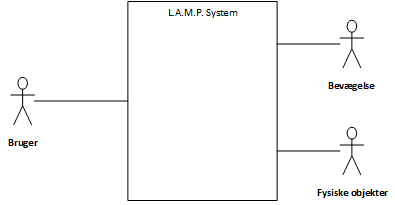
\includegraphics[width=\textwidth]{0_Filer/Figuer/AktoerKontekstLAMP.png}
    \caption{Kontekst diagram}
    \label{fig:kontekstdiagram}
\end{figure}

% Bruger
\begin{table}[H] \centering
\subsection{Bruger}
\begin{tabular}{|p{4cm}|p{8cm}|}
	\hline
	    \textbf{Alternativ reference}   & Ingen \\ \hline
	    \textbf{Type}                   & Primær \\ \hline
		\textbf{Beskrivelse}            & Brugeren interagerer med systemet via GUI. \\ \hline
	\end{tabular}
\end{table}

% Bevægelse
\begin{table}[H] \centering
\subsection{Bevægelse}
    \begin{tabular}{|p{4cm}|p{8cm}|}
	\hline
	    \textbf{Alternativ reference}   & Ingen \\ \hline
	    \textbf{Type}                   & Sekundær \\ \hline
		\textbf{Beskrivelse}            & Bevægelse i rummet vil aktivere bevægelsessensoren som vil tænde lys. \\ \hline
	\end{tabular}
\end{table}

% Fysiske Objekter
\begin{table}[H] \centering
\subsection{Fysiske Objekter}
\begin{tabular}{|p{4cm}|p{8cm}|}
	\hline
	    \textbf{Alternativ reference}   & Ingen \\ \hline
	    \textbf{Type}                   & Sekundær \\ \hline
		\textbf{Beskrivelse}            & Fysiske Objekter vil, hvis i en given afstand under lampen, stoppe nedadgående bevægelse. \\ \hline
	\end{tabular}
\end{table}
\clearpage

% 2.3 Usecases
\section{Usecases}

% Usecase diagram
\begin{figure}[H] \centering
    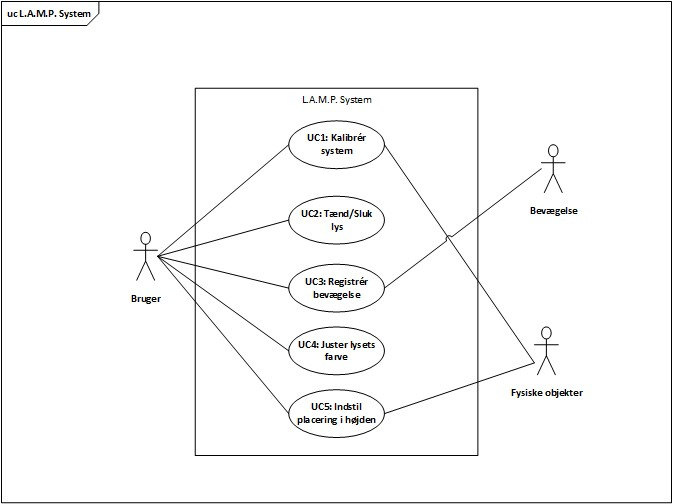
\includegraphics[width=\textwidth]{0_Filer/Figuer/ucLAMP3.jpg}
    \caption{Usecase diagram}
    \label{fig:usecasediagram}
\end{figure}

% UC1: Kalibrer system
\subsection{UC1: Kalibrer system}

\begin{center} \centering
	\begin{longtable}{|p{6cm}|p{8cm}|}
	\hline
		\multicolumn{2}{|l|}{\textbf{UC1: Kalibrer system}} \\\hline
		\endfirsthead
		
		\multicolumn{2}{l}{...fortsat fra forrige side} \\ \hline 
		\multicolumn{2}{|l|}{\textbf{UC1: Kalibrer system}} \\\hline
		\endhead	
		
		\multicolumn{2}{r}{fortsættes på næste side...} \\
        \endfoot
        \endlastfoot

        \textbf{Mål}								
            & Systemet bliver kalibreret og klar til brug.
        \\ \hline
        \textbf{Initialisering}					
            & Brugeren trykker på ”Kalibrer” på touchskærmen.
        \\ \hline
        \textbf{Aktører og Stakeholders}			
            & Bruger.
        \\ \hline
        \textbf{Referencer}						
            & Ingen.
        \\ \hline
        \textbf{Antal af samtidige hændelser}	
            & Ingen.
        \\ \hline
        \textbf{Forudsætning}					
            & Systemet er tændt og funktionsdygtigt.
        \\ \hline
        \textbf{Efterfølgende tilstand}			
            & Systemet er kalibreret og klar til brug.
        \\ \hline
        \textbf{Hovedforløb}						
            & 
            \begin{enumerate}
                \item Bruger trykker ”Kalibrer” på touchskærmen
                \item Z-Motor kører i top.
                \item Z-Motor registrerer når den rammer switchen i top, og sætter Z-værdien til nul på Z-PSoC'en
                \item X-motorerne kører i bund i den ene ende af skinnerne i loftet, og derefter til modsatte ende.
                \item Antal steps det tager X-motorerne at køre fra en ende til den anden gemmes på X-PSoC'en.
                \item Y-motoren kører i bund i den ene ende af skinnen, hvorefter den kører til den modsatte ende.
                \item Antal steps det tager Y-motorerne at køre fra en ende til den anden gemmes på Y-PSoC'en.
                \item Systemet er nu kalibreret og viser beskeden “Kalibrering udført” på touchskærmen.
            \end{enumerate}
        \\ \hline
        \textbf{Undtagelser}						
            & [Generel undtagelse 1: Kalibrering fejler]
            \begin{enumerate}
			    \item System stopper motorer
			    \item System viser beskeden “Kalibrering fejlet, tilkald tekniker” på touchskærmen.
		    \end{enumerate}
        \\ \hline
	\end{longtable}
	\label{UC1} 
\end{center}

% UC2: Tænd/Sluk lys
\subsection{UC2: Tænd/Sluk lys}

\begin{center} \centering
	\begin{longtable}{|p{6cm}|p{8cm}|}
	\hline
		\multicolumn{2}{|l|}{\textbf{UC2: Tænd/Sluk lys}} \\\hline
		\endfirsthead
		
		\multicolumn{2}{l}{...fortsat fra forrige side} \\ \hline 
		\multicolumn{2}{|l|}{\textbf{UC2: Tænd/Sluk lys}} \\\hline
		\endhead		

        \multicolumn{2}{r}{fortsættes på næste side...} \\
        \endfoot
        \endlastfoot
        
        \textbf{Mål}								
            & Brugeren får tændt eller slukket lampen.
        \\ \hline
        \textbf{Initialisering}					
            & Brugeren trykker på ”On”- eller ”Off”-knap på touchskærmen.
        \\ \hline
        \textbf{Aktører og Stakeholders}			
            & Bruger.
        \\ \hline
        \textbf{Referencer}						
            & Ingen.
        \\ \hline
        \textbf{Antal af samtidige hændelser}	
            & Ingen.
        \\ \hline
        \textbf{Forudsætning}					
            & Systemet er tændt og funktionsdygtigt. Touchskærmen viser 'Light'-fanen
        \\ \hline
        \textbf{Efterfølgende tilstand}			
            & Lampen har skiftet tilstand mellem slukket og tændt.
        \\ \hline
        \textbf{Hovedforløb}						
            & 
            \begin{enumerate}
                \item Brugeren indstiller en valgt farve via de tre RGB-sliders under 'Light'-fanen.
                \item Brugeren trykker Go-knappen.
                \item Brugeren trykker på ”On”- eller ”Off”-knap for lys.
                \item Lampen skifter tilstand.
            \end{enumerate}
        \\ \hline
        \textbf{Undtagelser}						
            & Ingen.
        \\ \hline
	\end{longtable}
	\label{UC2} 
\end{center}

% UC3: Registrér bevægelse
\subsection{UC3: Registrér bevægelse}

\begin{center} \centering
	\begin{longtable}{|p{6cm}|p{8cm}|}
	\hline
		\multicolumn{2}{|l|}{\textbf{UC3: Registrér bevægelse}} \\\hline
		\endfirsthead
		
		\multicolumn{2}{l}{...fortsat fra forrige side} \\ \hline 
		\multicolumn{2}{|l|}{\textbf{UC3: Registrér bevægelse}} \\\hline
		\endhead		

        \multicolumn{2}{r}{fortsættes på næste side...} \\
        \endfoot
        \endlastfoot
        
        \textbf{Mål}								
            & Systemet registrerer bevægelse og tænder Lampen.
        \\ \hline
        \textbf{Initialisering}					
            & Bevægelsessensor registrerer bevægelse.
        \\ \hline
        \textbf{Aktører og Stakeholders}			
            & Bevægelsessensor.
        \\ \hline
        \textbf{Referencer}						
            & Ingen.
        \\ \hline
        \textbf{Antal af samtidige hændelser}	
            & Ingen.
        \\ \hline
        \textbf{Forudsætning}					
            & Systemet er tændt og funktionsdygtigt. Touchskærmen viser 'Sensor'-fanen. Lampen er slukket og Movement detection slideren er sat til Off.
        \\ \hline
        \textbf{Efterfølgende tilstand}			
            & Lampen er tændt.
        \\ \hline
        \textbf{Hovedforløb}						
            &
            \begin{enumerate}
                \item Brugeren sætter Movement detection slideren på On.
                \item Bevægelsessensor registrerer bevægelse.
                \item Lampen tændes.
            \end{enumerate} 
        \\ \hline
        \textbf{Undtagelser}						
            & Ingen.
        \\ \hline
	\end{longtable}
	\label{UC3} 
\end{center}

% UC4: Juster lysets farve
\subsection{UC4: Juster lysets farve}

\begin{center} \centering
	\begin{longtable}{|p{6cm}|p{8cm}|}
	\hline
		\multicolumn{2}{|l|}{\textbf{UC4: Juster lysets farve}} \\\hline
		\endfirsthead
		
		\multicolumn{2}{l}{...fortsat fra forrige side} \\ \hline 
		\multicolumn{2}{|l|}{\textbf{UC4: Juster lysets farve}} \\\hline
		\endhead		

        \multicolumn{2}{r}{fortsættes på næste side...} \\
        \endfoot
        \endlastfoot
        
        \textbf{Mål}								
            & Brugeren får indstillet lysets farve til den valgte værdi.
        \\ \hline
        \textbf{Initialisering}					
            & Bruger trykker på touchskærmen.
        \\ \hline
        \textbf{Aktører og Stakeholders}			
            & Bruger.
        \\ \hline
        \textbf{Referencer}						
            & Ingen.
        \\ \hline
        \textbf{Antal af samtidige hændelser}	
            & Ingen.
        \\ \hline
        \textbf{Forudsætning}					
            & Systemet er tændt og funktionsdygtigt. Touchskærmen viser 'Light'-fanen.
        \\ \hline 
        \textbf{Efterfølgende tilstand}			
            & Brugeren har fået indstillet lysets farve til valgte tilstand.
        \\ \hline
        \textbf{Hovedforløb}						
            &
            \begin{enumerate}
                \item Bruger indstiller lysets farve på RGB-sliderne under 'Light'-fanen.
                \item Bruger trykker på Go-knappen.
                \item Lyset er nu justeret.
            \end{enumerate}
        \\ \hline
        \textbf{Undtagelser}						
            & Ingen.
        \\ \hline
	\end{longtable}
	\label{UC5} 
\end{center}

% UC5: Indstil placering af lampen
\subsection{UC5: Indstil placering i af lampen}

\begin{center} \centering
	\begin{longtable}{|p{6cm}|p{8cm}|}
	\hline
		\multicolumn{2}{|l|}{\textbf{UC5: Indstil placering af lampen}} \\\hline
		\endfirsthead
		
		\multicolumn{2}{l}{...fortsat fra forrige side} \\ \hline 
		\multicolumn{2}{|l|}{\textbf{UC5: Indstil placering af lampen}} \\\hline
		\endhead		

        \multicolumn{2}{r}{fortsættes på næste side...} \\
        \endfoot
        \endlastfoot
        
        \textbf{Mål}								
            & Brugeren har indstillet lampens placering i rummet.
        \\ \hline
        \textbf{Initialisering}					
            & Bruger trykker på touchskærmen.
        \\ \hline
        \textbf{Aktører og Stakeholders}			
            & Bruger.
        \\ \hline
        \textbf{Referencer}						
            & Ingen.
        \\ \hline
        \textbf{Antal af samtidige hændelser}	
            & Ingen.
        \\ \hline
        \textbf{Forudsætning}					
            & Systemet er tændt, kalibreret og funktionsdygtigt. Touchskærmen viser 'Position'-fanen.
        \\ \hline
        \textbf{Efterfølgende tilstand}			
            & Lampen hænger i en valgt position.
        \\ \hline
        \textbf{Hovedforløb}						
            &
            \begin{enumerate}
                \item Bruger sætter X, Y og Z sliderne til en valgt position under 'Position'-fanen.
                \item Bruger trykker på Go-knappen.
                \item Lampen flytter sig til den valgte position.
                [Undtagelse 1: Afstandssensor registrerer objekt]
            \end{enumerate}
        \\ \hline
        \textbf{Undtagelser}						
            & [Undtagelse 1: Afstandssensor registrerer objekt]
            \begin{enumerate}
			    \item System stopper Z-motoren.
			    \item Lampen hejses 1 cm op fra dens position.
		    \end{enumerate}
        \\ \hline
	\end{longtable}
	\label{UC6} 
\end{center}

% UC6: Indstil placering i loft
%\subsection{UC6: Indstil placering i højden}

\begin{center} \centering
	\begin{longtable}{|p{6cm}|p{8cm}|}
	\hline
		\multicolumn{2}{|l|}{\textbf{UC6: Indstil placering i højden}} \\\hline
		\endfirsthead
		
		\multicolumn{2}{l}{...fortsat fra forrige side} \\ \hline 
		\multicolumn{2}{|l|}{\textbf{UC6: Indstil placering i højden}} \\\hline
		\endhead		

        \multicolumn{2}{r}{fortsættes på næste side...} \\
        \endfoot
        \endlastfoot
        
        \textbf{Mål}								
            & Brugeren får hævet eller sænket lampen til den valgte højde.
        \\ \hline
        \textbf{Initialisering}					
            & Bruger trykker på touchskærmen.
        \\ \hline
        \textbf{Aktører og Stakeholders}			
            & Bruger.
        \\ \hline
        \textbf{Referencer}						
            & Ingen.
        \\ \hline
        \textbf{Antal af samtidige hændelser}	
            & Ingen.
        \\ \hline
        \textbf{Forudsætning}					
            & At systemet er tændt, kalibreret og funktionsdygtigt.
        \\ \hline		
        \textbf{Efterfølgende tilstand}	
            & Lampens højde er indstillet til det valgte niveau.
        \\ \hline
        \textbf{Hovedforløb}						
            &
            \begin{enumerate}
                \item Bruger ændre Z-slider positionen, i position tappen.
                \item Brugeren trykker på GO-kanppen, på position tappen. 
                    \newline [Undtagelse 1: Sensor registrerer forhindring]
                \item Lampe er nu indstillet til den valgte højde.
            \end{enumerate}
        \\ \hline
        \textbf{Undtagelser}						
            & [Undtagelse 1: Sensor registrerer forhindring]
            \begin{enumerate}
                \item Systemet stopper nedsænkningen af lampen og kan kun køre opad igen.
            \end{enumerate}
        \\ \hline
	\end{longtable}
	\label{UC7} 
\end{center}

% UC7: Indstil placering i højden
%\subsection{UC7: Tilføj plan}

\begin{center} \centering
	\begin{longtable}{|p{6cm}|p{8cm}|}
	\hline
		\multicolumn{2}{|l|}{\textbf{UC7: Tilføj plan}} \\\hline
		\endfirsthead
		
		\multicolumn{2}{l}{...fortsat fra forrige side} \\ \hline 
		\multicolumn{2}{|l|}{\textbf{UC7: Tilføj plan}} \\\hline
		\endhead		

        \multicolumn{2}{r}{fortsættes på næste side...} \\
        \endfoot
        \endlastfoot
        
        \textbf{Mål}								
            & En ny plan med position og lysindstillinger bliver oprettet på touchskærmen.
        \\ \hline
        \textbf{Initialisering}					
            & Bruger trykker på en plan under planner fanen på touchskærmen.
        \\ \hline
        \textbf{Aktører og Stakeholders}			
            & Bruger.
        \\ \hline
        \textbf{Referencer}						
            & Ingen.
        \\ \hline
        \textbf{Antal af samtidige hændelser}	
            & Ingen.
        \\ \hline
        \textbf{Forudsætning}					
            & At systemet er tændt og funktionsdygtigt.
        \\ \hline
        \textbf{Efterfølgende tilstand}			
            & En ny plan med systemets nuværende indstillinger er gemt på touchskærmen med et udvalgt navn.
        \\ \hline
        \textbf{Hovedforløb}						
            &
            \begin{enumerate}
                \item Bruger klikker Planner-fanen på touchskærmen.
                \item Bruger klikker ”Save location” på touchskærmen.
                \item Devkit8000 giver brugeren et nyt vindue hvor et udvalgt navn til planen kan indtastes
                \item Bruger indtaster et udvalgt navn i indtast- ningsfeltet ”Plan name:”.
                \item Bruger trykker på ”Save” i vinduet på touchskærmen.     \newline [Undtagelse 1: Bruger trykker ”Cancel”]
                \item Ny plan med udvalgte navn og nuværende indstillinger er oprettet og kan ses under Planner-fanen.
            \end{enumerate}
        \\ \hline
        \textbf{Undtagelser}						
            & [Undtagelse 1: Bruger trykker “Cancel”]
             \begin{enumerate}
                \item Bruger klikker på “Cancel”-knappen.
                \item Vinduet til oprettelse af plan på touchskærmen lukkes ned og ingen plan er gemt.
             \end{enumerate}
        \\ \hline
	\end{longtable}
	\label{UC8} 
\end{center}

% UC8: Tilføj plan
%\subsection{UC8: Vælg plan}

\begin{center} \centering
	\begin{longtable}{|p{6cm}|p{8cm}|}
	\hline
		\multicolumn{2}{|l|}{\textbf{UC8: Vælg plan}} \\\hline
		\endfirsthead
		
		\multicolumn{2}{l}{...fortsat fra forrige side} \\ \hline 
		\multicolumn{2}{|l|}{\textbf{UC8: Vælg plan}} \\\hline
		\endhead		

        \multicolumn{2}{r}{fortsættes på næste side...} \\
        \endfoot
        \endlastfoot
        
        \textbf{Mål}								
            & Systemet skifter position og lysindstillinger fra de nuværende til de udvalgte.
        \\ \hline
        \textbf{Initialisering}					
            & Bruger trykker på en plan under planner fanen på touchskærmen.
        \\ \hline
        \textbf{Aktører og Stakeholders}			
            & Bruger.
        \\ \hline
        \textbf{Referencer}						
            & Ingen.
        \\ \hline
        \textbf{Antal af samtidige hændelser}	
            & Ingen.
        \\ \hline
        \textbf{Forudsætning}					
            & At systemet er tændt, funktionsdygtigt, har en plan oprettet og har andre indstillinger end de udvalgte fra planen.
        \\ \hline
        \textbf{Efterfølgende tilstand}			
            & Systemet er nu indstillet til valgte tilstand.
        \\ \hline
        \textbf{Hovedforløb}						
            &
            \begin{enumerate}
                \item Bruger klikker Planner-fanen på touchskærmen.
                \item Bruger klikker en gemt plan på touchskærmen.
                \item Systemet er nu indstillet til indstillinger identiske til den udvalgte plan.
            \end{enumerate}
        \\ \hline
        \textbf{Undtagelser}						
            & Ingen.
        \\ \hline
	\end{longtable}
	\label{UC9} 
\end{center}

% UC9: Vælg plan
%\subsection{UC9: Vælg plan}

\begin{center} \centering
	\begin{longtable}{|p{6cm}|p{8cm}|}
	\hline
		\multicolumn{2}{|l|}{\textbf{UC9: Vælg plan}} \\\hline
		\endfirsthead
		
		\multicolumn{2}{l}{...fortsat fra forrige side} \\ \hline 
		\multicolumn{2}{|l|}{\textbf{UC9: Vælg plan}} \\\hline
		\endhead		

        \multicolumn{2}{r}{fortsættes på næste side...} \\
        \endfoot
        \endlastfoot
        
        \textbf{Mål}								
            & Systemet skifter position og lysindstillinger fra de nuværende til de udvalgte.
        \\ \hline
        \textbf{Initialisering}					
            & Bruger trykker på en plan under planner fanen på touchskærmen.
        \\ \hline
        \textbf{Aktører og Stakeholders}			
            & Bruger.
        \\ \hline
        \textbf{Referencer}						
            & Ingen.
        \\ \hline
        \textbf{Antal af samtidige hændelser}	
            & Ingen.
        \\ \hline
        \textbf{Forudsætning}					
            & At systemet er tændt, funktionsdygtigt, har en plan oprettet og har andre indstillinger end de udvalgte fra planen.
        \\ \hline
        \textbf{Efterfølgende tilstand}			
            & Systemet er nu indstillet til valgte tilstand.
        \\ \hline
        \textbf{Hovedforløb}						
            &
            \begin{enumerate}
                \item Bruger klikker Planner-fanen på touchskærmen.
                \item Bruger klikker en gemt plan på touchskærmen.
                \item Systemet er nu indstillet til indstillinger identiske til den udvalgte plan.
            \end{enumerate}
        \\ \hline
        \textbf{Undtagelser}						
            & Ingen.
        \\ \hline
	\end{longtable}
	\label{UC9} 
\end{center}
\clearpage

% 2.4 Ikke-funktionelle Krav
\section{Ikke-funktionelle krav}

\begin{enumerate}
	\subsection*{Brugbarhed (Usability)}
	    \item GUI skal kunne bruges efter gennemlæst manual.
	
	\subsection*{Pålidelighed (Reliability)}
	    \item Levetid: 5 år uden hardware nedbrud.
	    \item Software oppetid: Minimum 1 måned før genstart.
	
	\subsection*{Ydeevne (Performance)}
	    \item System respons må maksimalt være 2,5 sekunder.
	    \item Startuptid fra power-off til funktionel tilstand maksimalt 2 minutter.
	    \item Bevægelsessensoren skal kunne registrerer bevægelse i en afstand af op til 4 meter.

	\subsection*{Vedligeholdelse (Supportability)}
    	\item Systemet er plug’n’play i en almindelig husholdning.
	    \item Pære skal kunne udskiftes.
	    \item Basale fejl løses med hjælp fra manualen, ved andre fejl tilkaldes tekniker.

    \subsection*{Generelle krav}
	    \item Systemet skal virke på det eksisterende 230 Vac netværk i almindelige husstande.
	    \item Lampeskærm må ikke veje over 0,5 kg.
\end{enumerate}
\clearpage

% 2.5 Begrænsninger
\section{Begrænsninger}

\begin{enumerate}
	\item Prototypen udføres i et 5 VDC testmiljø.
	\item Pære udskiftes med tre styk RGB-led'er.
	\item Grundet prototypens størrelse, testes P.I.R. sensoren kun op til 1m.
\end{enumerate}
\clearpage

% 2.6 GUI
% \section{GUI}
Nedenstående sketch repræsenterer en foreløbig ide om, hvordan GUI’en skal se ud. Sketchen er baseret på den optimale udførelse af projektet, og medtager derfor funktioner som på nuværende tidspunkt ikke er defineret i usecases. Disse funktioner er "Could Haves", og vil evt. blive tilpasset senere. Planner tappen på nedestående figur er et eksempel på dette.

% GUI Controller
\begin{figure}[H] \centering
    \fbox{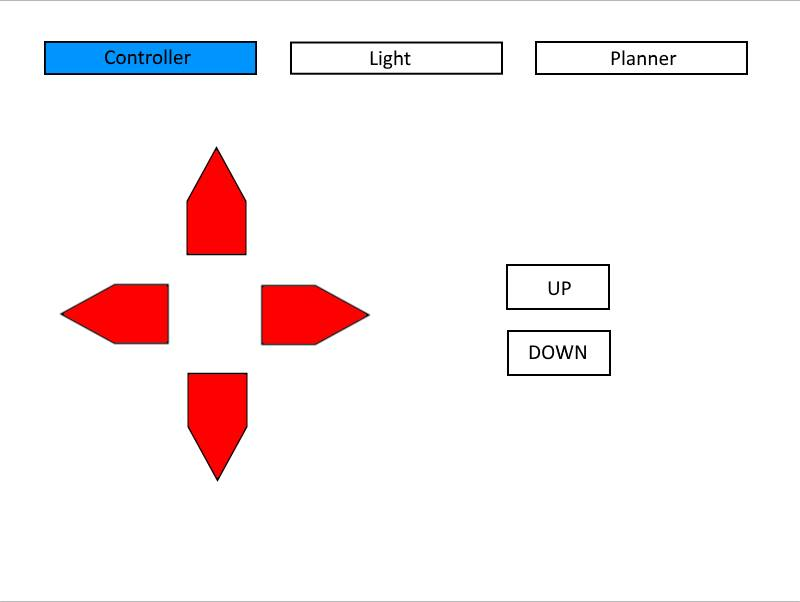
\includegraphics[width=0.6\textwidth]{0_Filer/Figuer/GUI1.jpg}}
    \caption{GUI Controller}
    \label{fig:GUIController}
\end{figure}

% GUI Lys
\begin{figure}[H] \centering
    \fbox{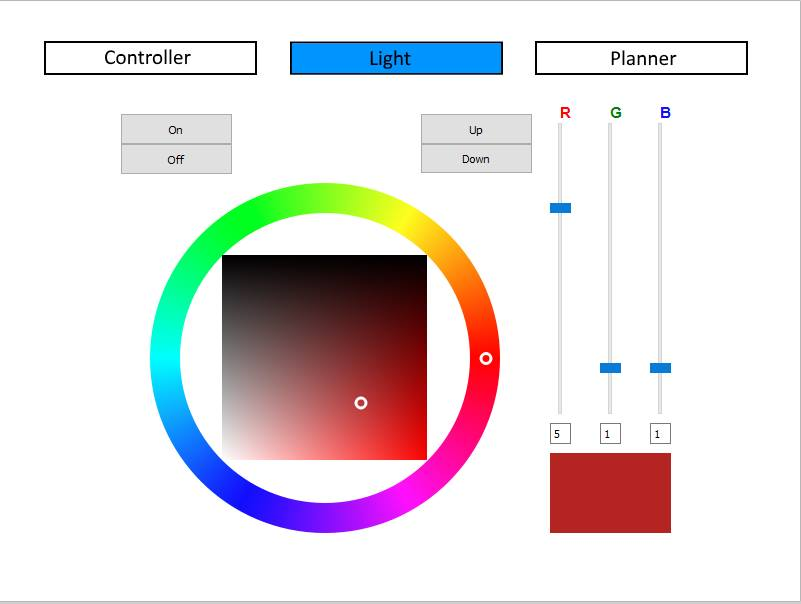
\includegraphics[width=0.6\textwidth]{0_Filer/Figuer/GUI2.jpg}}
    \caption{GUI Lys}
    \label{fig:GUILys}
\end{figure}
% \clearpage

% 3. Forundersøgelse
% 3. Forundersøgelse
\chapter{Forundersøgelse}

% 3.1 Motor XY
\section{XY motor}
Formålet med denne forundersøgelse er at se på forskellige typer af motorer, deres fordele og ulemper. Ud fra undersøgelsen vælges den motor der passer bedst i systemet.

Som udgangspunkt til undersøgelsen er motorene tilgængelige på embedded stock blevet undersøgt, men alternativer udenfor embedde stock er også blevet undersøgt. 

\begin{table}[H] \centering
\begin{tabular}{|p{3cm}|p{11cm}|}
	\hline
	\textbf{Løsning}		
	    & 12VDC Gearmotor 600:1
	\\ \hline
	\textbf{Producent} 		
	    & 
	\\ \hline
	\textbf{Interface} 		
	    & Spænding
	 \\ \hline
	\textbf{Beskrivelse} 	
	    & 
	\\ \hline
	\textbf{Krav} 			
	    & Kræver 12Volt DC - Stall Current: 1.6A
	\\ \hline
	\textbf{Fordele}		
	    & Kan stoppe på alle 360grd
	\\ \hline
	\textbf{Ulemper} 		
	    & 1 tilgængelig. meget kraftig motor. 12V.
	\\ \hline
	\textbf{Pris} 			
	    & Embedded stock, tilgængelig: 1
	\\ \hline
	\textbf{Link} 			
	    & \url{http://10.29.0.30/EmbeddedStock/Component?componentid=13985}
	\\ \hline
	\multicolumn{2}{|c|}{} 
    \\ \hline
\end{tabular}
\end{table}

\begin{table}[H] \centering
\begin{tabular}{|p{3cm}|p{11cm}|}
	\hline
	\textbf{Løsning}		
	    & 12VDC Motor (SL28S-10385-45C)
	\\ \hline
	\textbf{Producent} 		
	    & 
	\\ \hline
	\textbf{Interface} 		
	    & Spænding
	\\ \hline
	\textbf{Beskrivelse} 	
	    & 
	\\ \hline
	\textbf{Krav} 			
	    & Kræver 12Volt DC
	\\ \hline
	\textbf{Fordele}		
	    & Strømforbrug 0,119A, kan positioneres på alle 360 grd.
	\\ \hline
	\textbf{Ulemper} 		
	    & 12VDC
	\\ \hline
	\textbf{Pris} 			
	    & Embedded stock. tilgængelige: 23
	\\ \hline
	\textbf{Link} 			
	    & \url{http://10.29.0.30/EmbeddedStock/Component?componentid=13547} 
	\\ \hline
	\multicolumn{2}{|c|}{} 
    \\ \hline
\end{tabular}
\end{table}

\begin{table}[H] \centering
\begin{tabular}{|p{3cm}|p{11cm}|}
	\hline
	\textbf{Løsning}		
	    & 5VDC Stepmotor (28BYJ-48)
	\\ \hline
	\textbf{Producent} 		
	    & 
	\\ \hline
	\textbf{Interface} 		
	    & Spænding, position
	\\ \hline
	\textbf{Beskrivelse} 	
	    & Stepmotor
	\\ \hline
	\textbf{Krav} 			
	    & Kræver 5VDC
	\\ \hline
	\textbf{Fordele}		
	    & 5VDC, nem at styre positionering
	\\ \hline
	\textbf{Ulemper} 		
	    & Ingen datablad på embedded stock
	\\ \hline
	\textbf{Pris} 			
	    & Embedded stock, 9 tilgængelige.
	\\ \hline
	\textbf{Link} 			
	    & \url{}
	\\ \hline
	\multicolumn{2}{|c|}{} 
    \\ \hline
\end{tabular}
\end{table}

\begin{table}[H] \centering
\begin{tabular}{|p{3cm}|p{11cm}|}
	\hline
	\textbf{Løsning}		
	    & 6VDC Gearmotor 18:1
	\\ \hline
	\textbf{Producent} 		
	    & 
	\\ \hline
	\textbf{Interface} 		
	    & Spænding
	\\ \hline
	\textbf{Beskrivelse} 	
	    & 
	\\ \hline
	\textbf{Krav} 			
	    & Kræver 5VDC
	\\ \hline
	\textbf{Fordele}		
	    & Kan positioneres på alle 360 grd
	\\ \hline
	\textbf{Ulemper} 		
	    & Permanent omdrejningstal
	\\ \hline
	\textbf{Pris} 			
	    & Embedded stock. tilgængelige: 4
	\\ \hline
	\textbf{Link} 			
	    & \url{http://10.29.0.30/EmbeddedStock/Component?componentid=13984}
	\\ \hline
	\multicolumn{2}{|c|}{} 
    \\ \hline
\end{tabular}
\end{table}

\begin{table}[H] \centering
\begin{tabular}{|p{3cm}|p{11cm}|}
	\hline
	\textbf{Løsning}		
	    & NEMA17 Stepmotor V9728
	\\ \hline
	\textbf{Producent} 		
	    & 
	\\ \hline
	\textbf{Interface} 		
	    & Spænding, position
	\\ \hline
	\textbf{Beskrivelse} 	
	    & 
	\\ \hline
	\textbf{Krav} 			
	    & Kræver 12VDC, Rated Current 0.4A
	\\ \hline
	\textbf{Fordele}		
	    & Nem positionering, stepvinkel 1,8grd +/-5
	\\ \hline
	\textbf{Ulemper} 		
	    & Bruger 12VDCl
	\\ \hline
	\textbf{Pris} 			
	    & Embedded stock. tilgængelige: 6stk.
	\\ \hline
	\textbf{Link} 			
	    & \url{http://10.29.0.30/EmbeddedStock/Component?componentid=14179}
	\\ \hline
	\multicolumn{2}{|c|}{} 
    \\ \hline
\end{tabular}
\end{table}

\begin{table}[H] \centering
\begin{tabular}{|p{3cm}|p{11cm}|}
	\hline
	\textbf{Løsning}		
	    & RS-varenummer 781-3046 
	\\ \hline
	\textbf{Producent} 		
	    & Parallax inc.
	\\ \hline
	\textbf{Interface} 		
	    & Spænding, 3 benet konnektor, analogt feedback
	\\ \hline
	\textbf{Beskrivelse} 	
	    & 
	\\ \hline
	\textbf{Krav} 			
	    & +4 til +6VDC, 15 til 200mA
	\\ \hline
	\textbf{Fordele}		
	    & Nem positionering.
	\\ \hline
	\textbf{Ulemper} 		
	    & Dyr i økonomi.
	\\ \hline
	\textbf{Pris} 			
	    & 94,85kr.
	\\ \hline
	\textbf{Link} 			
	    & \url{http://dk.rs-online.com/web/p/servomotorer/7813046/}
	\\ \hline
	\multicolumn{2}{|c|}{} 
    \\ \hline
\end{tabular}
\end{table}

\begin{table}[H] \centering
\begin{tabular}{|p{3cm}|p{11cm}|}
	\hline
	\textbf{Løsning}		
	    & Analog feedback mikro servomotor m. plast gear + tilbehør 
	\\ \hline
	\textbf{Producent} 		
	    & Adafruit
	\\ \hline
	\textbf{Interface} 		
	    & Spænding, analogt feedback
	\\ \hline
	\textbf{Beskrivelse} 	
	    & 
	\\ \hline
	\textbf{Krav} 			
	    & Max 6VDC
	\\ \hline
	\textbf{Fordele}		
	    & Nem positionering. lav vægt.
	\\ \hline
	\textbf{Ulemper} 		
	    & Dyr i indkøb.
	\\ \hline
	\textbf{Pris} 			
	    & 139,00kr.
	\\ \hline
	\textbf{Link} 			
	    & \url{}
	\\ \hline
	\multicolumn{2}{|c|}{} 
    \\ \hline
\end{tabular}
\end{table}

\subsection{Valg af XY motor}
5VDC Stepmotor (28BYJ-48)
med 3072 steps pr. omgang til præcis og nem styring af position og tilgænglig på embedded stock.
\clearpage

% 3.2 Sensor Lys
\section{Lys sensor}
Udgangspunktet for denne undersøgelse er så vidt som muligt at bruge de komponenter vi har til rådighed i Embedded Stock. Hvilket umiddelbart betyder lyssensore af typerne: TEMT6000, TSL2561, og TCS230.

Undersøgelsen har som mål at finde sensorer der (i prioriteret rækkefølge):
\begin{enumerate}
    \item Har gode egenskaber inden for det synlige spektrum (ca. 400 – 700 nm).
    \item Kan tilgås med en interessant protokol – I2C er foretrukket.
    \item Er i stand til at måle farvetemperaturer.
\end{enumerate}

\begin{table}[H] \centering
\begin{tabular}{|p{3cm}|p{11cm}|}
	\hline
	\textbf{Løsning}		
	    & TEMT6000 
	\\ \hline
	\textbf{Producent} 		
	    & Vishay Semiconductors 
	\\ \hline
	\textbf{Interface} 		
	    & Analog output (strøm, typisk: 10-50 µA) 
	\\ \hline
	\textbf{Beskrivelse} 	
	    & Simpel sensor, der måler lysintensitet 
	\\ \hline
	\textbf{Krav} 			
	    & Opfylder krav 1 
	\\ \hline
	\textbf{Fordele}		
	    & Simpel, fornuftig spektrum responskurve 
	\\ \hline
	\textbf{Ulemper} 		
	    & Lidt for simpel kommunikation, responskurve strækker sig lidt over i det infrarøde område, kan ikke måle farver 
	\\ \hline
	\textbf{Pris} 			
	    & Tilgængelig i Embedded Stock 
	\\ \hline
	\textbf{Link} 			
	    & \url{https://www.sparkfun.com/datasheets/Sensors/Imaging/TEMT6000.pdf} 
	\\ \hline
	\multicolumn{2}{|c|}{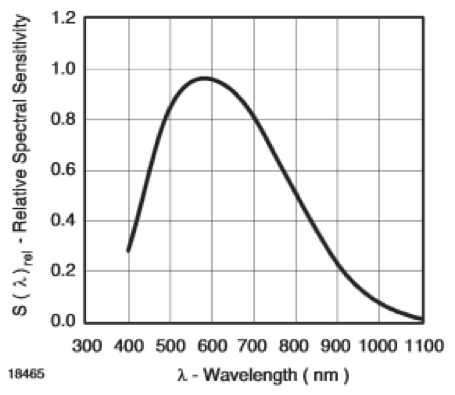
\includegraphics[height=6cm]{0_Filer/Figuer/Forudundersoegelse/TEMT6000.png}} 	
    \\ \hline
\end{tabular}
\end{table}

\begin{table}[H] \centering
\begin{tabular}{|p{3cm}|p{11cm}|}
	\hline
	\textbf{Løsning}		
	    & TSL2561 
	\\ \hline
	\textbf{Producent} 		   
	    & Texas Advanced Optoelectronic Solutions Inc. 
	\\ \hline
	\textbf{Interface} 		
	    & I2C 
	\\ \hline
	\textbf{Beskrivelse} 	
	    & Udstyret med to sensorer: En til synligt + infrarødt lys og en kun til infrarødt lys. Designet til at man tager målingen fra den første sensor og fratrækker målingen fra den anden (ligninger findes i databladet) 
	\\ \hline
	\textbf{Krav} 			
	    & Opfylder krav 1 og 2 
	\\ \hline
	\textbf{Fordele}		
	    & Burde give en fornuftig spektrum responskurve efter korrigering, bruger I2C protokol 
	\\ \hline
	\textbf{Ulemper} 		
	    & Kan ikke måle farver, kræver noget ekstra kode til korrektion 
	\\ \hline
	\textbf{Pris} 			
	    & Tilgængelig i Embedded Stock 
	\\ \hline
	\textbf{Link} 			
	    & \url{https://www.adafruit.com/datasheets/TSL2561.pdf}
	\\ \hline
	\multicolumn{2}{|c|}{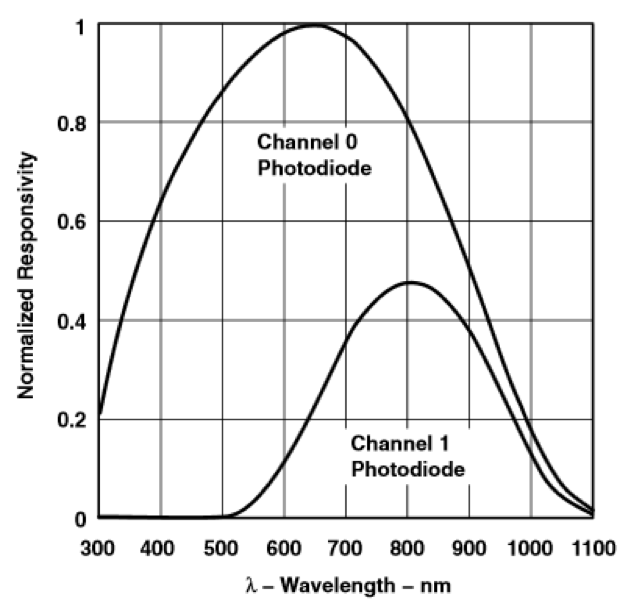
\includegraphics[height=6cm]{0_Filer/Figuer/Forudundersoegelse/TSL2561.png}} 	
    \\ \hline
\end{tabular}
\end{table}

\begin{table}[H] \centering
\begin{tabular}{|p{3cm}|p{11cm}|}
	\hline
	\textbf{Løsning}		
	    & TCS230 \\ \hline
	\textbf{Producent} 		
    	& Texas Advanced Optoelectronic Solutions Inc. 
    \\ \hline
	\textbf{Interface} 		
    	& 50\% PWM firkantsignal der ændre frekvens efter målt lysintensitet 
    \\ \hline
	\textbf{Beskrivelse} 	
    	& Udstyret med fire sensor blokke til rød, blå, grøn og hvidt (ingen filter) lys 
    \\ \hline
	\textbf{Krav} 			
    	& Opfylder krav 3 
    \\ \hline
	\textbf{Fordele}		
    	& Kan måle farver og ikke kun generel lysintensitet 
    \\ \hline
	\textbf{Ulemper} 		
	    & Har en meget dårligt spektrum responskurve, der ligger meget langt ovre i det infrarøde spektrum 
	\\ \hline
	\textbf{Pris} 			
	    & Tilgængelig i Embedded Stock 
	\\ \hline
	\textbf{Link} 			
	    & \url{http://www.pobot.org/IMG/pdf/tcs230_datasheet.pdf}
	\\ \hline
	\multicolumn{2}{|c|}{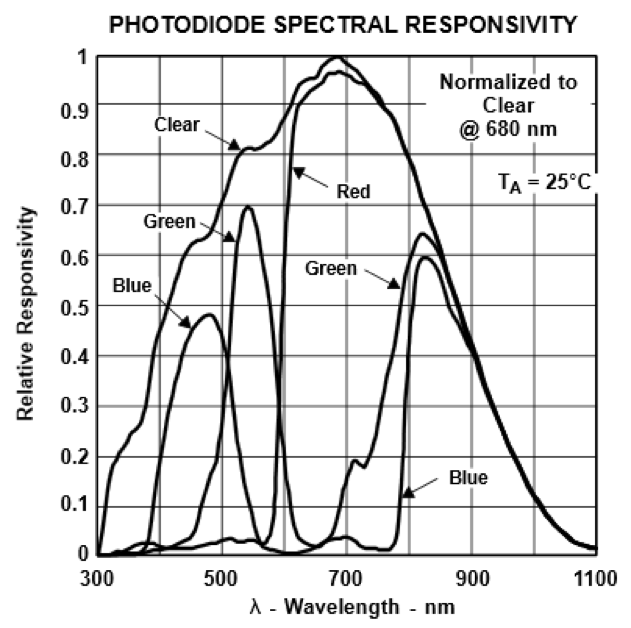
\includegraphics[height=6cm]{0_Filer/Figuer/Forudundersoegelse/TCS230.png}} 	
    \\ \hline
\end{tabular}
\end{table}

\begin{table}[H] \centering
\begin{tabular}{|p{3cm}|p{11cm}|}
	\hline
	\textbf{Løsning}		
		& TCS230 + eksternt filter (datasheet foreslåer: Hoya CM500) 
	\\ \hline
	\textbf{Producent} 		
		& Texas Advanced Optoelectronic Solutions Inc. 
	\\ \hline
	\textbf{Interface} 		
		& 50\% PWM firkantsignal der ændre frekvens efter målt lysintensitet
	\\ \hline
	\textbf{Beskrivelse} 	
		& Udstyret med fire sensor blokke til rød, blå, grøn og hvidt (ingen filter) lys 
	\\ \hline
	\textbf{Krav} 			
		& Opfylder krav 1 og 3 
	\\ \hline
	\textbf{Fordele}		
		& Kan måle farver og ikke kun generel lysintensitet. Meget god spektrum responskurve 
	\\ \hline
	\textbf{Ulemper} 		
		& Kræver indkøb af eksternt filter 
	\\ \hline
	\textbf{Pris} 			
		& Sensor: Tilgængelig i Embedded Stock. Eksternt filter: 180-190 kr. 
    \\ \hline
    \textbf{Link} 			
        & \url{http://www.pobot.org/IMG/pdf/tcs230_datasheet.pdf}
	\\ \hline
	\multicolumn{2}{|c|}{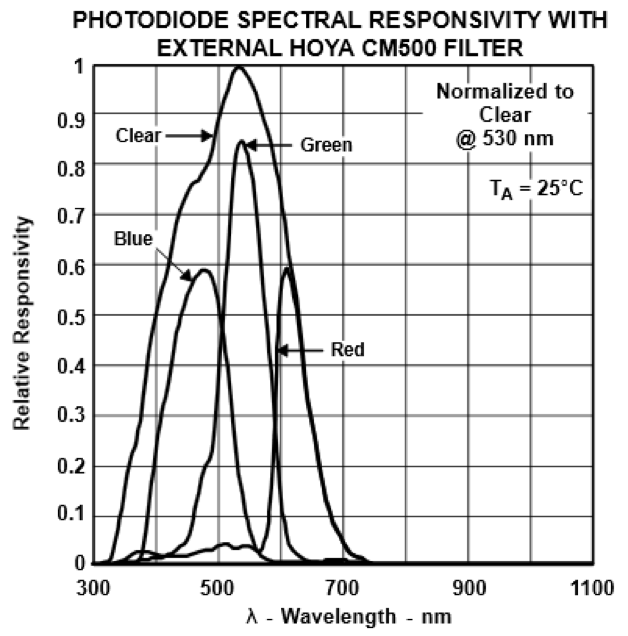
\includegraphics[height=6cm]{0_Filer/Figuer/Forudundersoegelse/TCS230-CM500.png}} 	
    \\ \hline
\end{tabular}
\end{table}

\subsection{Valg af lys sensoren}

Efter at have gennemgået databladende for alle tre sensorer, er konklusionen at arbejde videre med TSL2561 sensoren, da den umiddelbart opfylder de fleste af vores krav. Men hvis ikke kommunikationen eller differensberegningerne vil komme til at virke er TEMT6000 også en brugbar mulighed.

På den anden side, må TCS230 afvises medmindre der kan skaffes et eksternt IR filter til den.
\clearpage

% 3.3 PIR Sensor
\section{PIR sensor}

Udgangspunktet for denne undersøgelse er så vidt som muligt at bruge de komponenter vi har til rådighed i Embedded Stock. Hvilket umiddelbart betyder en PIR sensor af typen:

\begin{table}[H] \centering
\begin{tabular}{|p{3cm}|p{11cm}|}
	\hline
	\textbf{Løsning}		
	    & HC-SR501, PIR-bevægelsessensor
	\\ \hline
	\textbf{Producent} 		
	    & Ukendt
	\\ \hline
	\textbf{Interface} 		
	    & TTL 
	\\ \hline
	\textbf{Beskrivelse} 	
	    & En PIR-sensor der giver et High output når bevægelse er registeret. High er 3.3 V, og Low er 0 V
	\\ \hline
	\textbf{Krav} 			
	    & Godt kendskab til PSoC creator
	\\ \hline
	\textbf{Fordele}		
	    & Denne PIR-sensor kræver ingen ekstra HW. Justerbar delay og range via potentiometer
	\\ \hline
	\textbf{Ulemper} 		
	    & Begrænset præcision og rækkevidde
	\\ \hline
	\textbf{Pris} 			
	    & Ved lavpris elektronik: 59,- (Hentet gratis på EL-lab)
	\\ \hline
	\textbf{Link} 			
	    & \url{https://www.mpja.com/download/31227sc.pdf} 
	\\ \hline
	\multicolumn{2}{|c|}{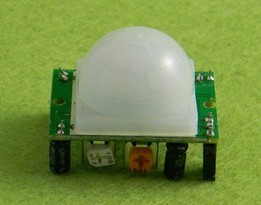
\includegraphics[width=0.3\linewidth]{0_Filer/Figuer/Forudundersoegelse/PIR_sensor_billede.jpg}}
    \\ \hline
\end{tabular}
\end{table}

\subsection{Konklusion}

HC-SR501 PIR-bevægelsessensor opfylder alle de behov der er brug for i vores projekt. Den er lille og kompakt og følsomhed/forsinkelse kan let indstilles. Da sensoren er tilgængelig på Embedded stock, er denne valgt.

\clearpage

% 3.3 Afstandssensor
\section{Afstandssensor}

Udgangspunktet for denne undersøgelse er så vidt som muligt at bruge de komponenter vi har til rådighed i Embedded Stock. Hvilket umiddelbart betyder en Ultra Sonisk sensor af typen:

\begin{table}[H] \centering
\begin{tabular}{|p{3cm}|p{11cm}|}
	\hline
	\textbf{Løsning}		
	    & HC-SR04 Ultra Sonic Sensor
	\\ \hline
	\textbf{Producent} 		
	    & Elec Freaks
	\\ \hline
	\textbf{Interface} 		
	    & TTL\footcite{ttl}
	\\ \hline
	\textbf{Beskrivelse} 	
	    & Sensoren trigges med en 10uS TTL puls, hvorefter sensoren udsender et sonar signal på 40kHz. Output fra sensoren er en TTL puls af samme varighed som det tager Sensoren at modtage et ekko
	\\ \hline
	\textbf{Krav} 			
	    & Godt kendskab til PSoC creator
	\\ \hline
	\textbf{Fordele}		
	    & Denne sensor kræver ingen ekstra HW. Den er simpel i brug, stabil og præcis
	\\ \hline
	\textbf{Ulemper} 		
	    & Begrænset målevinkel
	\\ \hline
	\textbf{Pris} 			
	    & Ved lavpris elektronik: 59,- (Hentet gratis på EL-lab)
	\\ \hline
	\textbf{Link} 			
	    & \url{http://www.micropik.com/PDF/HCSR04.pdf}
	\\ \hline
	\multicolumn{2}{|c|}{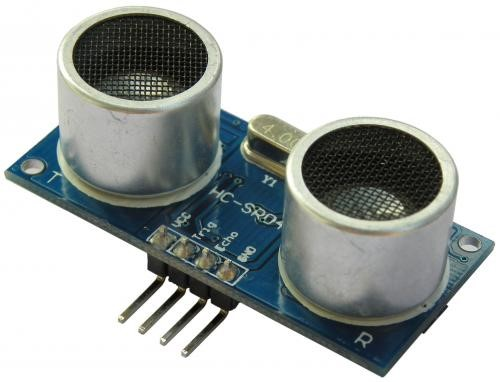
\includegraphics[width=0.3\linewidth]{0_Filer/Figuer/Forudundersoegelse/Afstandssensor_billede.jpg}}
    \\ \hline
\end{tabular}
\end{table}

\subsection{Konklusion}

HC-SR04 Ultra Sonic sensor opfylder alle de behov der er brug for til projektet. Den er stabil og præcis og kræver ikke ekstra hardware. Da sensoren er tilgængelig på Embedded stock, er denne blevet valgt.

\clearpage


% 4. Systemarkitektur
% 4. Systemarkitektur
\chapter{Systemarkitektur}

Systemarkitekturen består af en række forskellige diagrammer med dertilhørende tekst.
Diagrammerne er opbygget efter SysML standarden\footnote{ISE undervisningen på 2. semester}

% 4.1 Domænemodel
\section{Domænemodel}

% Domænemodel
\begin{figure}[H] \centering
    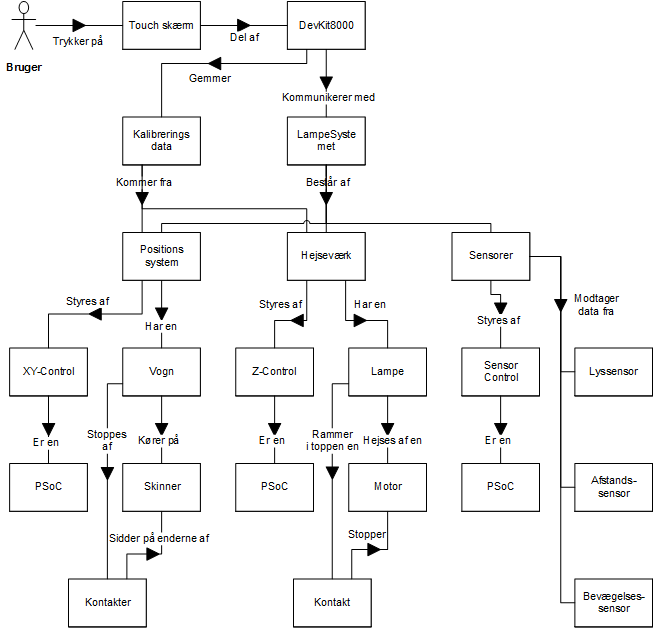
\includegraphics[width=\textwidth]{0_Filer/Figuer/DomaenemodelLAMP.png}
    \caption{Domænemodel}
    \label{fig:domaenemodel}
\end{figure}


Domænemodellen i figur \ref{fig:domaenemodel} beskriver systemets funktionalitet og de forskellige deles indbyrdes sammenhæng.
\clearpage

% 4.2 Hardware beskrivelse
\section{Hardware beskrivelse}

% BDD  L.A.M.P.
\subsection{BDD L.A.M.P.}
\begin{figure}[H] \centering
    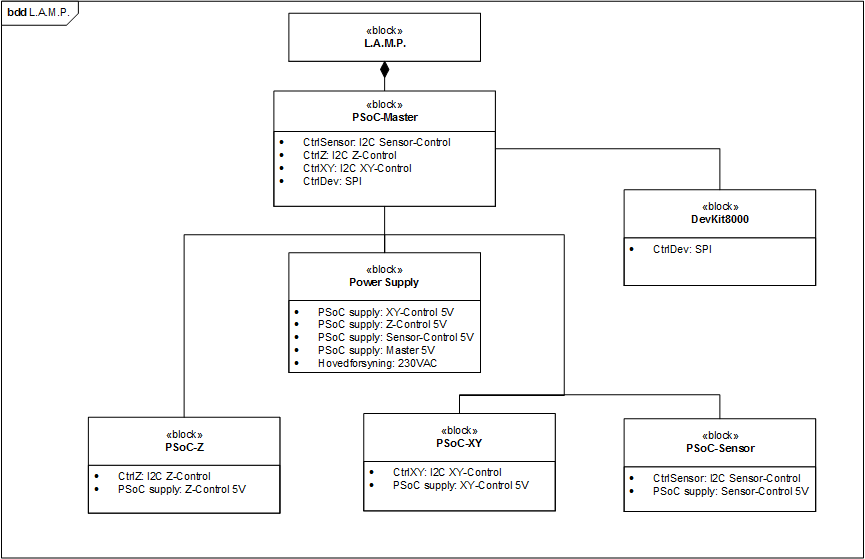
\includegraphics[width=\textwidth]{0_Filer/Figuer/5_HW_Design/bddLAMPvers2.png}
    \caption{BDD L.A.M.P.}
    \label{fig:bddLAMP}
\end{figure}
I figur \ref{fig:bddLAMP} er blok definitions diagrammet over det overordnede L.A.M.P system, diagrammet indeholder signal navne og forbindelserne mellem blokkene.

% BDD  XY-Control
\subsection{BDD XY-Control}
\begin{figure}[H] \centering
    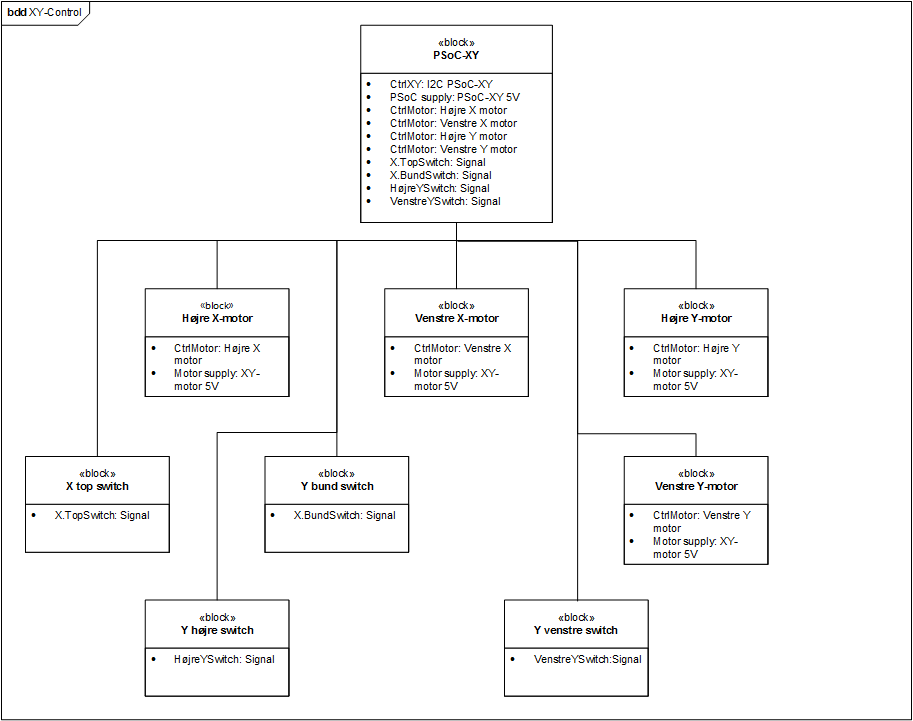
\includegraphics[width=\textwidth]{0_Filer/Figuer/5_HW_Design/bddPSoC1vers2.png}
    \caption{BDD XY-Control}
    \label{fig:bddXY}
\end{figure}
I figur \ref{fig:bddXY} er blok definitions diagrammet for XY-Control, den består af en PSoC der styre X og Y motorerne, diagrammet indeholder signal navne og forbindelserne mellem blokkene.

% BDD  Z-Control
\subsection{BDD Z-Control}
\begin{figure}[H] \centering
    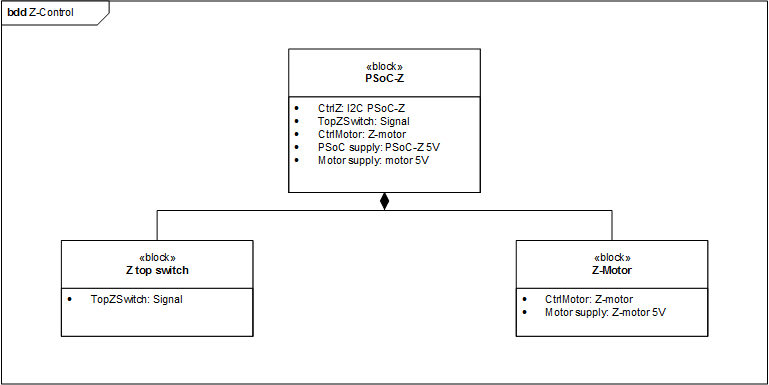
\includegraphics[width=\textwidth]{0_Filer/Figuer/5_HW_Design/bddPSoC2vers2.png}
    \caption{BDD Z-Control}
    \label{fig:bddZ}
\end{figure}
I figur \ref{fig:bddZ} er blok definitions diagrammet for Z-Control, den består af en PSoC der styre Z motoren og selve lampen, diagrammet indeholder signal navne og forbindelserne mellem blokkene.

% BDD Sensor-Control
\subsection{BDD Sensor-Control}
\begin{figure}[H] \centering
    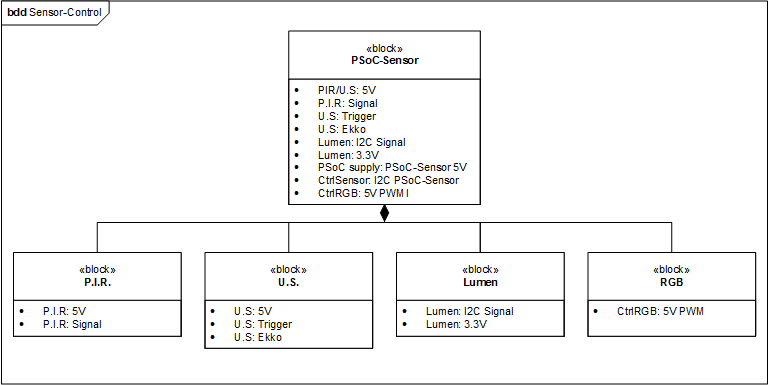
\includegraphics[width=\textwidth]{0_Filer/Figuer/5_HW_Design/bddPSoC3vers2.png}
    \caption{BDD Sensor-Control}
    \label{fig:bddSensor}
\end{figure}
I figur \ref{fig:bddSensor} er blok definitions diagrammet for Sensor-Control, den består af en PSoC der modtager information fra sensorerne, diagrammet indeholder signal navne og forbindelserne mellem blokkene.

% IBD L.A.M.P.
\subsection{IBD L.A.M.P.}
\begin{figure}[H] \centering
    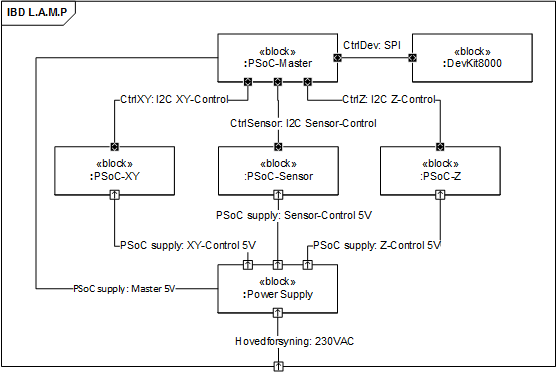
\includegraphics[width=\textwidth]{0_Filer/Figuer/5_HW_Design/IBD_LAMP_vers3.png}
    \caption{IBD L.A.M.P.}
    \label{fig:ibdLAMP}
\end{figure}
I figur \ref{fig:ibdLAMP} er det interne blok diagram over hele systemet L.A.M.P, diagrammet indeholder signal navne og forbindelserne mellem blokkene.

% IBD XY-Control
\subsection{IBD XY-Control}
\begin{figure}[H] \centering
    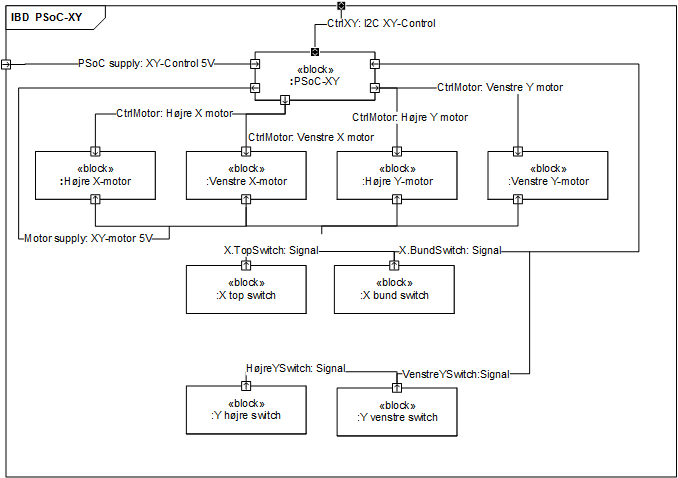
\includegraphics[width=\textwidth]{0_Filer/Figuer/5_HW_Design/IBD_PSoC1_vers3.png}
    \caption{IBD XY-Control}
    \label{fig:ibdXY}
\end{figure}
I figur \ref{fig:ibdXY} er det interne blok diagram for PSoC1, denne PSoC styre X og Y motorerne, diagrammet indeholder signal navne og forbindelserne mellem blokkene.

% IBD Z-Control
\subsection{IBD Z-Control}
\begin{figure}[H] \centering
    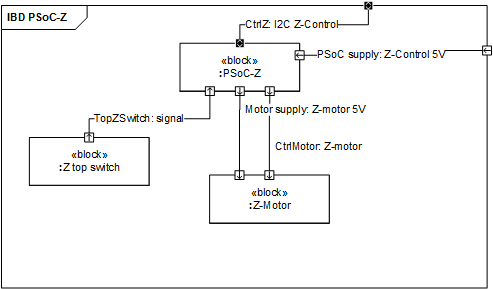
\includegraphics[width=\textwidth]{0_Filer/Figuer/5_HW_Design/IBD_PSoC2_Z_vers3.png}
    \caption{IBD Z-Control}
    \label{fig:ibdZ}
\end{figure}
I figur \ref{fig:ibdZ} er det interne blok diagram for PSoC2, denne PSoC styre Z motoren og selve lampen, diagrammet indeholder signal navne og forbindelserne mellem blokkene.

% IBD Sensor-Control
\subsection{IBD Sensor-Control}
\begin{figure}[H] \centering
    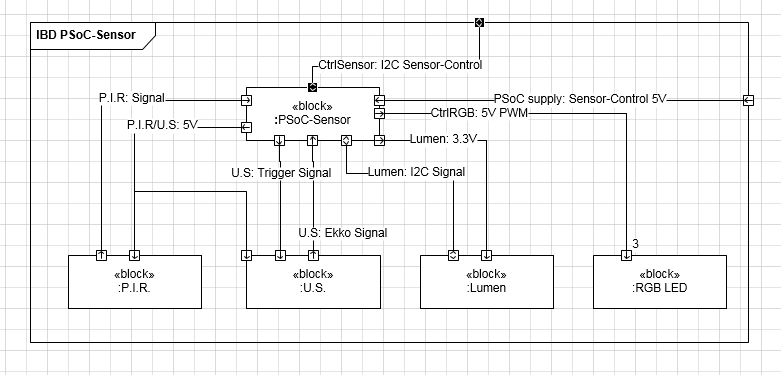
\includegraphics[width=\textwidth]{0_Filer/Figuer/5_HW_Design/IBD_sensor_vers3.png}
    \caption{IBD Sensor-Control}
    \label{fig:ibdSensor}
\end{figure}
I figur \ref{fig:ibdSensor} er det interne blok diagram for PSoC3, denne PSoC modtager information fra sensorerne, diagrammet indeholder signal navne og forbindelserne mellem blokkene.

% Grænseflade
\subsection{Grænseflade}

% PSoC-Master
\subsubsection{PSoC-Master}
1 PSoC, 1 stk. Nokia 5110 display.
\begin{itemize}
    \item PSoC-Master står for kommunikationen mellem Devkit8000 og XY-, Z- og Sensor PSoCs.
    \item Nokia 5110 diplay brugt til debugging til at kontrollere kommunikationen mellem Devkit8000 og PSoC-Master.
     PSoC-manual\footnote{\url{http://www.cypress.com/file/46056/download}}
\end{itemize}

% XY-Control
\subsubsection{PSoC-XY}
1 PSoC, 2 stk. X-motorer, 2 stk. Y-motor, 8 stk. MosFet, 4 stk. XY-Switches.
\begin{itemize}
    \item PSoC leverer styresignal til MosFets for at styre motorerne
    \item MosFet1-4 leverer spænding til 2 motorer for at styre bevægelse. (X-akse)
    \item MosFet5-8 leverer spænding til 2 motorer for at styre bevægelse. (Y-akse)
    \item PSoC’en overvåger to X og to Y switches for registrering af lampens yderste positioner. 
\end{itemize}

% Z-Control
\subsubsection{PSoC-Z}
1 PSoC, 1 Z-motor, 4 stk. MosFet, Z-Switch.
\begin{itemize}
    \item PSoC levere styresignal til MosFets for at styre motoren (Z-akse).
    \item PSoC’en overvåger Z-Switch for registrering af lampens øverste position.
\end{itemize}

% Sensor-Control
\subsubsection{PSoC-Sensor}
1 PSoC, 1 stk. lyssensor, 1 stk. afstandsmåler, 1 stk. bevægelsessensor.
\begin{itemize}
    \item PSoC’en kommunikerer med Lyssensor, afstandsmåler og bevægelsessensor via I2C-protokol.
    \item PSoC leverer spænding til Lyssensor
    \item PSoC leverer spænding til afstandsmåler
    \item PSoC leverer spænding til bevægelsessensor
\end{itemize}

% Devkit8000
\subsubsection{Devkit8000}
1 Devkit8000.
\begin{itemize}
    \item Devkit8000 er forsynet med strøm fra egen forsyning
    \item Devkit8000 kommunikerer med PSoC-Master via SPI
\end{itemize}

% Power Supply
\subsubsection{Power Supply}
Strømforsyning.
\begin{itemize}
    \item Fabrikeret strømkilde i form af en USB hub leverer 5V til PSOCs. 
    \item Devkit8000 har sin egen strømforsyning.
\end{itemize}


\subsubsection{Bloktabel}
For at opnå forståelse for signalerne mellem blokkene laves en grænseflade beskrivelse, der beskriver de enkelte blokkes porte og hvilke signaler der sendes imellem disse. 

Til at beskrive blokkene nærmere anvendes tabel \ref{tab:bloktabel} Her er hvert signal i hver deres respektive blokke kommenteret og blokkens funktion er kort beskrevet. 

\begin{center} \centering
    \begin{longtable}{|p{3,3cm}|p{3,3cm}|p{3,3cm}|p{3,3cm}|} \hline
	\textbf{Bloknavn} & \textbf{Funktion} & \textbf{Signaler} & \textbf{Kommentar} \\ \hline
	\endfirsthead
		
	\multicolumn{4}{l}{...fortsat fra forrige side} \\ \hline 
	\textbf{Bloknavn} & \textbf{Funktion} & \textbf{Signaler} & \textbf{Kommentar} \\ \hline
	\endhead

	\multicolumn{4}{r}{fortsættes på næste side...} \\
    \endfoot
    \endlastfoot
        
        Devkit8000
        & At kommunikere brugerens input fra touchskærmen ud til PSoC-Master
        & Input: Touch
        & Touch fra bruger
        \\ \cline{3-4}
        &
        & Output: SPI
        & SPI til PSoC-Master
        \\ \hline
        
        PSoC-Master(PSoC)
        & At kommunikere brugerens input fra touchskærmen ud til korrekte enheder og indhente data fra PSoC-enhederne
        & Input: SPI
        & 
        \\ \cline{3-4}
        &
        & Output: I2C
        & I2C til PSoC-enhederne
        \\ \hline
        
        PSoC-XY(PSoC)
        & At styre motorerne og dermed flytte vognen på skinnesystemet i rummets X- og Y-retning.
        & Input: I2C
        & I2C fra Master
        \\ \cline{3-4}
        &
        & Output: 5V og 3.3V
        & 5V til motorerne, 3.3V til switches
        \\ \hline
        
        PSoC-Z(PSoC)
        & At hæve og sænke lampen i rummets Z-akse. 
        & Input: I2C
        & I2C fra Master og et TTL\footcite{ttl} signal fra PSoC-Sensor
        \\ \cline{3-4}
        &
        & Output: 5V og 3.3V
        & 5V til motor, 3.3V til switches
        \\ \hline
        
        PSoC-Sensor(PSoC)
        & At aflæse og levere data fra dens tilkoblede sensorer til PSoC-Master og PSoC-Sensor, samt lysstyring af LED.
        & I/O: I2C 
        & I2C til sensorerne
        \\ \cline{3-4}
        &
        & Input: I2C
        & I2C fra PSoC-Master
        \\ \cline{3-4}
        &
        & Output: TTL signal og 0-5V  
        & TTL signal til PSoC-Z, samt 0-5V til RGB dioderne.
        \\ \hline
        
        Strømforsyning
        & At forsyne PSoC-enhederne med strøm
        & Output: 5V
        & 5V til PSoC-enhederne
        \\ \hline
        
        X-, Y-Motor
        & At flytte vognen i rummets X- og Y-akse
        & Input: 5V
        & Styresignal og driftspænding fra PSoC  
        \\ \hline
        
        Z-Motor
        & At flytte lampen på rummets Z-akse.
        & Input: 5V
        & Styresignal og driftspænding fra PSoC
        \\ \hline
        
        PIR-sensor
        & Detekterer bevægelser
        & I/O: TTL
        & TTL fra PSoC-Sensor
        \\ \hline
        
        Ultra-sonic (afstandsmåler)
        & Måler afstanden fra lampens nederste kant og ned til objekt.
        & I/O: TTL
        & TTL fra PSoC-Sensor
        \\ \hline
        
        TSL2561 (lysmåler)
        & Måler rummets lysniveau
        & I/O: I2C
        & I2C fra PSoC-Sensor
        \\ \hline
        
        Switches
        & Skaber forbindelse ved yderposition af vogn og lampe på X-, Y-, og Z-aksen
        & I/O: On/Off
        &
        \\ \hline
        
        RGB LED
        & Lyser rummet op i det ønskede farvespektrum
        & Input: Red - 1,9V, Green - 3V og Blue - 3V
        & Bliver styret af Sensor PSoC’en
        \\ \hline
    \caption{Bloktabel}
	\label{tab:bloktabel} 
    \end{longtable}
\end{center}

% Signalbeskrivelse
\subsection{Signalbeskrivelse}

For at fuldende beskrivelsen af grænsefladen er der lavet en signaltabel \ref{tab:signaltabel}. Hvert signal er beskrevet, og området et signal er defineret under, er også beskrevet. Blok og terminal indgår også. 
\begin{center} \centering
    \begin{longtable}{|p{2,6cm}|p{2,6cm}|p{2,6cm}|p{2,6cm}|p{2,6cm}|}\hline
	\textbf{Signalnavn} & \textbf{Funktion} & \textbf{Område} & \textbf{Port 1} & \textbf{Port 2} \\ \hline
	\endfirsthead
		
	\multicolumn{5}{l}{...fortsat fra forrige side} \\ \hline 
	\textbf{Signalnavn} & \textbf{Funktion} & \textbf{Område} & \textbf{Port 1} & \textbf{Port 2} \\ \hline
	\endhead
	
	\multicolumn{5}{r}{fortsættes på næste side...} \\
    \endfoot
    \endlastfoot

        I2C
        & Seriel 2-wire kommunikation
        & 
        & PSoC-Master, PSoC-Z
        & PSoC-XY, PSoC-Z, PSoC-Sensor, Lumen sensor
        
        \\ \hline 
        
        TTL
        & Højt/Lavt signal
        & 5V
        & PSoC-Sensor
        & PIR og Afstandssensor
        
        \\ \hline 
        
        SPI
        & Seriel 4-wire kommunikation
        &
        & Devkit8000
        & PSoC-Master 
        \\ \hline 
        
        5V
        & Forsyning til motor
        & 0V til 5V
        & PSoC-XY, PSoC-Z
        & Motor
        \\ \hline
        
        Max 3V
        & Forsyning til LED
        & 0V til 3V
        & PSoC-Sensor
        & LED
        \\ \hline
        
        5V
        & Forsyning til PSoC
        & 5V
        & Strømforsyning
        & PSoC-XY 
            \newline PSoC-Z
            \newline PSoC-Sensor
        \\ \hline
        
        On/Off
        & Bryde eller afbryde et signal
        & On/Off
        & PSoC-XY
            \newline PSoC-Z
        & PSoC-XY 
            \newline PSoC-Z
        \\ \hline
	\caption{Signaltabel}
	\label{tab:signaltabel} 
    \end{longtable}
\end{center}
\clearpage

% 4.3 Software beskrivelse
\section{Software beskrivelse}

For at danne overblik over software-udviklingen inden det egentlige design, anvendes N+1 modellen\footnote{4+1 architectural view model \url{https://en.wikipedia.org/wiki/4\%2B1_architectural_view_model}}. Denne beskriver fire faser som tager hånd om de overordnede ting inden for software, alt sammen med usecases som den røde tråd. De fire faser er:
\begin{enumerate}
    \item Logical View
    \item Deployment View
    \item Implementation View 
    \item Data View
\end{enumerate}
Disse punkter er beskrevet i detaljer herefter.

% Logical View
\subsection{Logical View}
Logical View skal danne et overblik over hvilke softwarepakker der befinder sig på platforme. Blokkene inde i de respektive pakker kan sammen med domænemodellen, hjælpe med at give et overblik over hvilke klasser og kernemoduler der skal bruges.
% Logical View Devkit8000
\subsubsection{Logical View Devkit8000}
\begin{figure}[H] \centering
    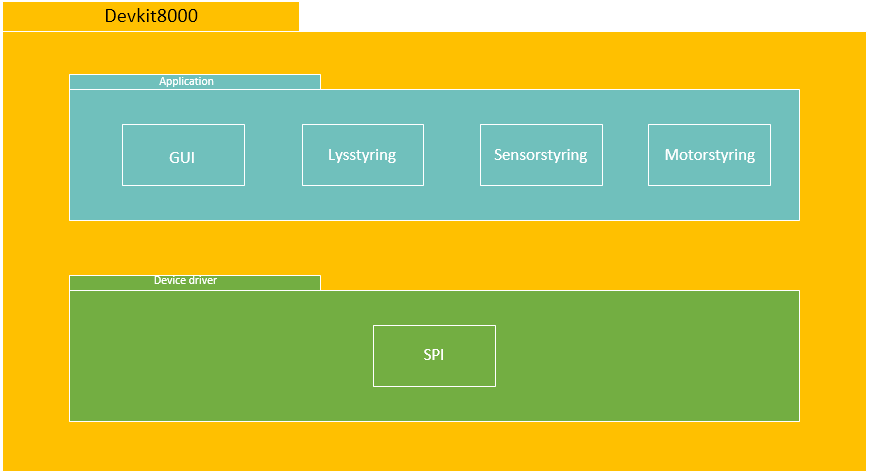
\includegraphics[width=\textwidth]{0_Filer/Figuer/LogicalViewDevkit8000.png}
    \caption{Logical View Devkit8000}
    \label{fig:LogicalView}
\end{figure}
Figur \ref{fig:LogicalView} illustrerer hvilke softwarepakker der ligger på Devkit8000. I bunden er Hardware API-pakken som håndterer protokol-vedtægter ifm. kommunikationen. I midten ligger Device drivers-pakken som håndterer protokol kommunikationen mellem Devkit8000 og PSoC. Application-pakken tager sig af alt UI samt kalibrering, sensorstyring og motorstyring.

% Logical View PSoC
\subsubsection{Logical View PSoC}
\begin{figure}[H] \centering
    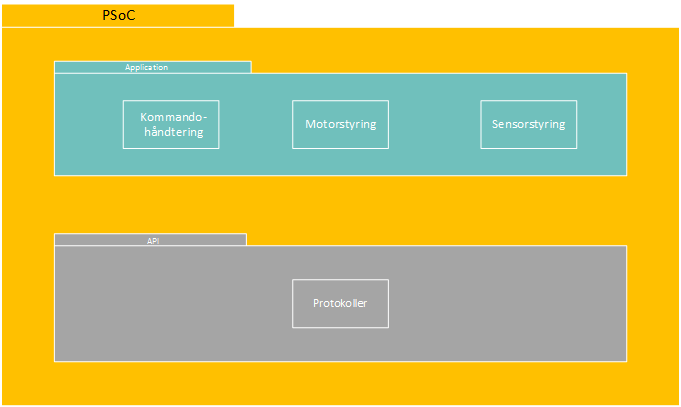
\includegraphics[width=\textwidth]{0_Filer/Figuer/LogicalViewPSoC.png}
    \caption{Logical View PSoC}
    \label{fig:LogicalViewPSoC}
\end{figure}
Figur \ref{fig:LogicalViewPSoC} illustrerer hvilke softwarepakker der ligger på PSoC. I bunden er en API-pakke som håndterer protokol-vedtægter ifm. kommunikationen. Øverst er application-pakken der tager sig af alt kommandohåndtering, motorstyring og sensorstyring.

% Deployment View
\subsection{Deployment View}
% DeploymentView
\subsubsection{DeploymentView}
\begin{figure}[H] \centering
    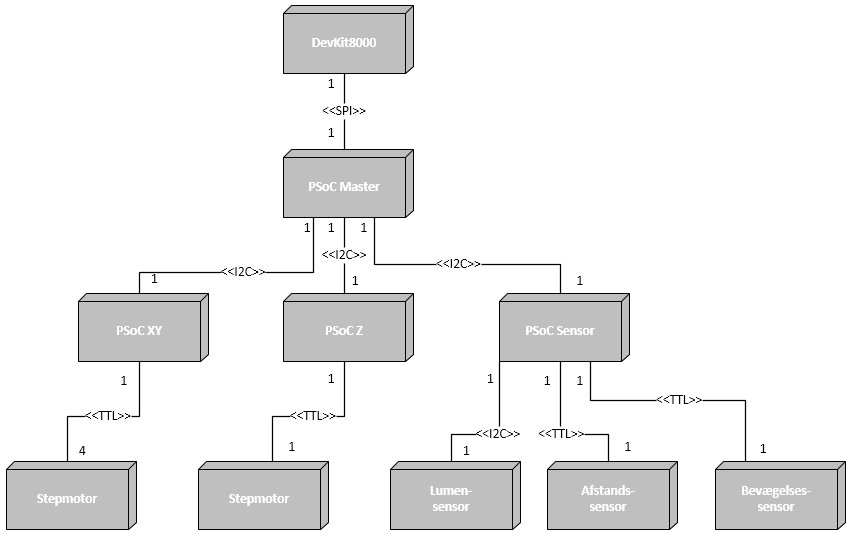
\includegraphics[width=\textwidth]{0_Filer/Figuer/DeploymentView.png}
    \caption{DeploymentView}
    \label{fig:DeploymentView}
\end{figure}


% Implementation View
\subsection{Implementation View}
Inden programmerne designes, fastlægges en struktur for kildekoden. På den måde er det nemmere for flere programmører at arbejde med delene i programmet samtidigt.
Strukturen skal være som vist i figur \ref{fig:ImplementationView}. Under mappen ”Kildekode” skal hver klasse have en mappe med dertil hørende filer. Ligeledes med ”Testprogrammer” mappen, som indholder testprogrammer som verificerer funktionaliteten af de enkelte moduler. Mappen ”Kompilerede programmer” er til de endelige programmer.
% Implementation View
\begin{figure}[H] \centering
    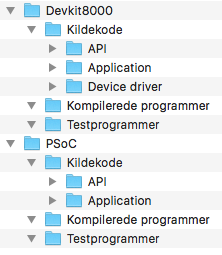
\includegraphics[width=0.4\textwidth]{0_Filer/Figuer/ImplementationView.png}
    \caption{Implementation View}
    \label{fig:ImplementationView}
\end{figure}


% Data View
\subsection{Data View}
I forbindelse med L.A.M.P. drift skal der gemmes data på en nem og håndterbar måde. Det skal være muligt at gemme følgende data:
\begin{enumerate}
    \item Position på X-motor
    \item Position på Y-motor
    \item Position på Z-motor
    \item Lysstyrke
    \item Lysets farve
    \item Kalibrerings data
\end{enumerate}
\clearpage

% 4.4 Protokol
\section{Protokol}

En del data skal flyttes mellem DevKit, PSoC-Master med SPI og mellem PSoC-Master og PSoC-XY, PSoC-Z og PSoC-Sensor med I2C. Her følger beskrivelsen af hvordan kommunikationen over hhv. SPI og I2C forgår.

\subsection{SPI}

Opsætning er som følger:
\begin{itemize}
    \item Hastighed: 1 MHz
    \item SPI mode: 3 (CPOL 1 - CPHA 1)
    \item Antal bits: 16
\end{itemize}

Hastigheden er valgt på baggrund af Hal Exercise7\footnote{Hardware abstraktioner. Exercise 7: LDD with SPI. Øvelse med SPI Kommunikation}, PSoC kan dog køre med op til 8 MHz, men der er valgt en lavere hastighed da det vil give en større stabilitet.

\subsubsection{Kommandoer til SPI}

\subsection{I2C}

\begin{table}[H]
\caption{Master sender en commando og tilhørende værdi}
\centering
\begin{tabular}{|c|c|c|c|c|c|c|c|c|c|c|c|c|c|c|c|c|c|}
\hline 
\multicolumn{8}{|c|}{1. Byte} & ACK & \multicolumn{8}{|c|}{2. Byte} & ACK \\
\hline 
\textbf{7} & \textbf{6} & \textbf{5} & \textbf{4} & \textbf{3} & \textbf{2} & \textbf{1} & \textbf{0} & \textbf{} & \textbf{7} & \textbf{6} & \textbf{5} & \textbf{4} & \textbf{3} & \textbf{2} & \textbf{1} & \textbf{0} & \textbf{} \\
\hline 
MSB & & & & & & & LSB & & \multicolumn{8}{|c|}{Most signifiant  byte} & \\ 
\hline
\multicolumn{8}{|c|}{1. Byte send to slave} & by & \multicolumn{8}{|c|}{2. Byte send to slave} & by \\
\hline
\multicolumn{7}{|c|}{Adress slave} & R/W & slave & \multicolumn{8}{|c|}{Command send to slave} & slave\\
\hline \hline
\multicolumn{8}{|c|}{3. Byte} & ACK & \multicolumn{8}{|c|}{4. Byte} & ACK \\
\hline
\textbf{7} & \textbf{6} & \textbf{5} & \textbf{4} & \textbf{3} & \textbf{2} & \textbf{1} & \textbf{0} & \textbf{} & \textbf{7} & \textbf{6} & \textbf{5} & \textbf{4} & \textbf{3} & \textbf{2} & \textbf{1} & \textbf{0} & \textbf{} \\
\hline
\multicolumn{8}{|c|}{} & & \multicolumn{8}{|c|}{} & \\
\hline
\multicolumn{8}{|c|}{Data send to slave} & by & \multicolumn{8}{|c|}{Data send to slave} & by \\
\hline
\multicolumn{8}{|c|}{3. Byte send to slave} & slave & \multicolumn{8}{|c|}{4. Byte send to slave} & slave \\
\hline \hline
\multicolumn{8}{|c|}{5. Byte} & ACK & \multicolumn{8}{|c|}{} & \\
\hline
\textbf{7} & \textbf{6} & \textbf{5} & \textbf{4} & \textbf{3} & \textbf{2} & \textbf{1} & \textbf{0} & \textbf{} & \multicolumn{8}{|c|}{} & \textbf{} \\
\hline
\multicolumn{8}{|c|}{Least signifiant  byte} & & \multicolumn{8}{|c|}{} & \\
\hline
\multicolumn{8}{|c|}{Data send to slave} & by & \multicolumn{8}{|c|}{} & \\
\hline
\multicolumn{8}{|c|}{5. Byte send to slave} & slave & \multicolumn{8}{|c|}{} & \\
\hline
\end{tabular}
\label{tabel:I2CMasterData}
\end{table} 

\begin{table}[H]
\caption{2. Master modtager data}
\centering
\begin{tabular}{|c|c|c|c|c|c|c|c|}
\hline 
\textbf{7} & \textbf{6} & \textbf{5} & \textbf{4} & \textbf{3} & \textbf{2} & \textbf{1} & \textbf{0}\\ 
\hline 
MSB & & & & & & & LSB \\ 
\hline
\multicolumn{8}{|c|}{Byte read from slave} \\
\hline
\end{tabular}
\label{tabel:I2CMasterCommando}
\end{table} 

Efter hver modtaget byte sender masteren en ACK til slaven ved at sætte SDA lav og generere en clock-puls. Herefter overtager slaven igen SDA.
Efter sidste modtaget byte, sender masteren i stedet STOP ved at sætte SCL høj og derefter SDA høj og bussen er derefter frigivet igen.
\clearpage

% 5. Hardware design
% 5. Hardware design
\chapter{Hardware design}

\section{Design}

\subsection{Prototypemodel}

Til prototypen skal der designes nogle hardware dele. Designet af disse dele tager udgangspunkt i prototypen. Denne inkluderer et Devkit8000, som skal kommunikere med en PSoC-Master via. SPI kommunikation. PSoC-Master kommunikere med tre slaver via. I2C. Disse tre slaver styrer hver deres del af systemet, henholdsvis XY retningerne, Z retningen og sensorene.
\newline Til styring af XY og Z retningen bruges der sammenlagt 5 stk 5V DC stepper motorer af typen 28BYJ-48 samt et motor-styringsmodul til hver bevægelsesretning. 
\newline På PSoC-Sensor er der koblet en PIR sensor(HC-SR501), en lys sensor(TSL2561), en ultralyds sensor(HC-SR04) og 3 RGB dioder til lys.
\newline De enkelte dele af prototypen beskrives her under. 

\clearpage

\subsection{Kommunikationsbus}

Til projektet bruges to forskellige typer bus\footcite{gfv}. Mellem DevKit8000 og PSoC-Master benyttes SPI, og mellem PSoC-Master og de tre andre PSoCs (XY, Z og Sensor), samt mellem PSoC-Sensor og nogle af vores sensorer benyttes I2C.

Denne konfiguration er valgt, fordi det kunne være interessant at prøve at bruge mere end én type bus, og fordi det giver en fornuftig afkobling mellem brugerinterfacet på DevKit8000 og resten af systemet. Denne afkobling kunne derefter, i en videreudvikling af systemet, konverteres fra SPI til en form for wireless kommunikation – for eksempel Wifi eller Bluetooth.

\subsubsection{Serial Peripheral Interface (SPI)}

Serial Peripheral Interface (SPI) er en 4-wire, seriel data bus, der understøtter fuld duplex kommunikation mellem en enkelt master enhed og flere slave enheder\footcite{gfv}.

Hardwaremæssigt kræver SPI fire ledninger fra master enheden til slave enhederne (der findes også specielle konfigurationer med færre ledninger, men dem kommes der ikke ind på her):

\begin{itemize}
    \item SCLK - Serial clock
    \item MISO - Master In, Slave Out
    \item MOSI - Master Out, Slave In
    \item SS - Slave Select (active low)
\end{itemize}

De første tre linjer er fælles for alle enheder på bussen, mens der skal være en Slave Select per slave der skal kunne adresseres.

Selve kommunikationen foregår ved at master vælger en slave ved at sætte slavens SS lav, og derefter sender master taktslag på SCLK. For hvert taktslag bliver der overført en bit fra master til slaven i MOSI, og en bit fra slaven til master i MISO. Dette foregår typisk ved hjælp af skifteregistre, arrangeret så de former en ringbuffer.

\begin{figure}[H] \centering
    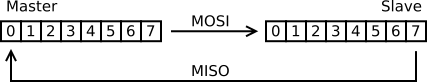
\includegraphics{0_Filer/Figuer/5_HW_Design/SPI_ringbuffer.png}
    \caption{SPI skifteregister ringbuffer}
    \label{fig:HWD_SPI_ring}
\end{figure}

Da kommunikationslinjerne er delte kræver det, at alle slaver på bussen ignorere data på SCLK og MOSI, og holder MISO som høj impedans så længe deres SS er inaktiv – dvs. så længe master enheden ikke har udvalgt dem.

SPI kommunikation har flere fordele:

\begin{itemize}
    \item Fuld duplex
    \item Meget simpel adressering – sæt et signal lavt, ingen behov for at bruge tid på at sende adresser
    \item Meget simpel protokol – ingen formelle krav om formattering, kan sende data med vilkårlige bitlængder
    \item Høj hastighed
\end{itemize}

Men der er også nogle ulemper ved SPI:

\begin{itemize}
    \item Adresseringen bruger et kabel, og en IO pind på master, per slave (kan undgås med daisy-chaining, men det øger kompleksiteten af protokollen og stiller krav til slavernes opførsel)
    \item Den meget simple protokol giver ingen hjælp til detektion af eller robusthed overfor fejl.
    \item Kun master enheden kan starte kommunikationen – hvis en slave vil sende noget til master enheden, må den vente på at masteren initierer, og slaver kan slet ikke kommunikerer med hinanden direkte.
\end{itemize}

\subsubsection{Inter-Integrated Circuit (I2C)}

Inter-Integrated Circuit (I\textsuperscript{2}C eller I2C) er en 2-wire, seriel bus, der understøtter halv duplex kommunikation mellem flere enheder\footcite{gfv} – i princippet er alle enheder lige i I2C, men i praksis vil de oftest være delt ind i masters og slaver ligesom i SPI, dog med den undtagelse at I2C understøtter flere masters på en bus og at enheder kan skifte roller.

Hardwaremæssigt kræver I2C kun to ledninger, der er delt mellem alle enheder på bussen. Dog skal de begge have en pull-up modstand, så de bliver holdt høj, når de er idle. De to linjer er:

\begin{itemize}
    \item SCL - Serial Clock Line
    \item SDA - Serial Data Line
\end{itemize}

\begin{figure}[H] \centering
    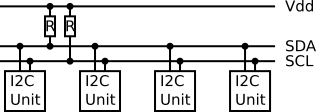
\includegraphics{0_Filer/Figuer/5_HW_Design/I2C_opsaetning.png}
    \caption{Eksempel på I2C kredsløb}
    \label{fig:HWD_I2C_kreds}
\end{figure}

I I2C følger kommunikationen en fast protokol, hvor den enhed der gerne vil initiere kommunikationen (master) først signalerer en start sekvens, og derefter sender data på SDA mens SCL laver et taktslag for hver bit. For at sørge for at der ikke kommer nogen falske aflæsninger af data, så er konventionen at SDA sætter det ønskede niveau på SCL falling-edge, og at SDA aflæses på rising-edge.

Den data der sendes er også underlagt en fast protokol: Den første byte, der bliver sendt skal bestå af først en 7-bit adresse på den enhed, som masteren gerne vil kommunikerer med (slaven), efterfulgt af en læse/skrive bit (0 = skrive til slaven, 1 = læse fra slaven). Derefter begynder den skrivende enhed at sende data på SDA i hele bytes, mens master enheden holder takten på SCL. Desuden bliver der, gennem hele forløbet transmitteret en acknowledge bit af den modtagende enhed efter hver hele byte der bliver modtaget.

Til sidst, når master enheden syntes at kommunikationen er færdig, laver master en stop sekvens, der frigiver bussen så en anden enhed kan komme til.

Et par eksempler på hvordan protokollen kører (hvide felter skrives af master, grå af slave):

\begin{figure}[H] \centering
    
\includegraphics{0_Filer/Figuer/5_HW_Design/I2C_Write.png}
    \caption{I2C Master skriver til slave}
    \label{fig:HWD_I2C_write}
\end{figure}

\begin{figure}[H] \centering
    
\includegraphics{0_Filer/Figuer/5_HW_Design/I2C_Read.png}
    \caption{I2C Master læser fra slave}
    \label{fig:HWD_I2C_read}
\end{figure}

\begin{figure}[H] \centering
    
\includegraphics{0_Filer/Figuer/5_HW_Design/I2C_Mixed.png}
    \caption{I2C Master skriver en byte til, derefter læser en byte fra slave}
    \label{fig:HWD_I2C_blandet}
\end{figure}

Figur \ref{fig:HWD_I2C_blandet} giver et eksempel på hvordan en sammenhængende kommunikation kan have data i begge retninger, uden at bussen frigives imellem ændringerne i dataflow retningen.

De umiddelbare fordele ved I2C er:

\begin{itemize}
    \item Understøttelse for flere master enheder
    \item Software addressering er fleksibel
    \item Det kræver ikke ekstra kabler eller IO pins at sætte en ekstra enhed på bussen
    \item Alle enheder kan tale direkte med hinanden
    \item Byte-ACK protokollen sikre den overordnede integritet af kommunikationen
\end{itemize}

Men I2C har også nogle ulemper og begrænsninger:

\begin{itemize}
    \item Ingen fuld duplex
    \item Lav hastighed i forhold til SPI
    \item Byte-ACK protokollen giver meget ringe beskyttelse overfor bit-fejl og generel data korruption.
\end{itemize}

\clearpage

\subsection{Komponentbeskrivelser}

\subsubsection{Lumen sensor}

Lumen sensoren der er valgt til projektet kommunikerer over I2C, og har dermed de fire standard ben: VDD og GND til forsyning samt SDA og SCL til I2C kommunikationen. Derudover har den to ekstra ben: ADDR-SEL som bruges til at vælge mellem tre forskellige addresser, så konflikter kan undgås, og INT som sensoren kan bruge til at sende en interrupt, hvis den funktionalitet bliver aktiveret.

Forsyningsspændingen skal ligge mellem 2.7 og 3.6 V, og sensoren bruger max 0.6 mA.

I kommunikationen med sensoren er der brug for to generelle funktioner:

\begin{enumerate}
    \item Skrive noget kontroldata til sensoren for at justerer dens opførsel
    \item Læse data fra sensoren for enten at verificerer at kontroldata er korrekt modtaget, eller at aflæse målinger
\end{enumerate}

Formatet for funktionerne er (grå felter bliver sendt af sensoren):

\begin{figure}[H] \centering
    
\includegraphics{0_Filer/Figuer/5_HW_Design/Lumen_skriv.png}
    \caption{Skrive kontroldata til sensor}
    \label{fig:HWD_Lumen_skriv}
\end{figure}

\begin{figure}[H] \centering
    
\includegraphics[width=\textwidth]{0_Filer/Figuer/5_HW_Design/Lumen_laes.png}
    \caption{Læse data fra sensor}
    \label{fig:HWD_Lumen_laes}
\end{figure}

Når sensoren først tændes starter den i power-down mode, derefter kan sensor funktionaliteten startes ved at sende en I2C kommando til den (kommando: 0x80 og data: 0x03). Efter sensoren er blevet sat til at køre kan dens to kanaler aflæses med I2C (kommando: 0xAC eller 0xAE).

De to output kanaler giver lysmålinger i det synlige + infrarøde område (kanal 0), og det infrarøde område (kanal 1). Så de to aflæsninger skal kombineres  for at få et tal kun for mængden af det synlige lys.

\begin{figure}[H] \centering
    
\includegraphics{0_Filer/Figuer/5_HW_Design/Kombinerings_formler.png}
    \caption{Kombinerings formler}
    \label{fig:HWD_Lumen_formler}
\end{figure}

\subsubsection{Afstandssensor}

Den valgte afstandssensor til projektet er af typen HC-SR04. Sensoren er en ultralyds sensor, som bruger sonar til kontaktfri afstandsmåling. Sensorens arbejdsfrekvens ligger på 40 kHz og output er et TTL signal.

Sensoren har 4 ben, VCC, GND, Trig og Echo som vist på billedet.

\begin{figure}[H] \centering
    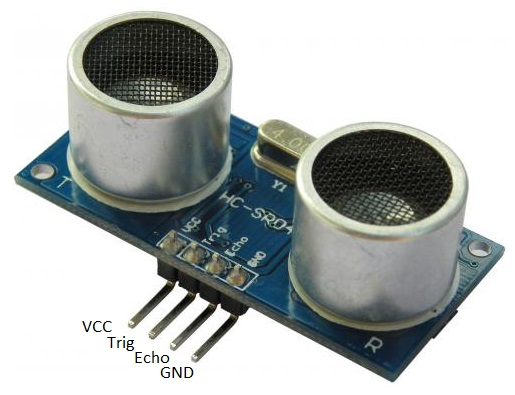
\includegraphics{0_Filer/Figuer/5_HW_Design/HC-SR04.jpg}
    \caption{HC-SR04 afstandssensor}
    \label{fig:HWD_SR04}
\end{figure}

Sensoren har en opløsning på 0,3 cm og er stabil og præcis i intervallet 2 cm til 400 cm, og måler i en vinkel på 15$^{\circ}$. Sensoren skal aktiveres med en TTL puls på mindst 10 mikrosekunder ind på Trig benet. Output fra sensoren kommer som et TTL signal på Echo benet, der har samme længde som tiden fra udsendt sonar burst til ekkosignal modtages af sensoren.

HC-SR04 skal forsynes med 5 VDC, har en idle current på under 2 mA og en working current på 15 mA.

Omregning af output fra sensoren til afstand i cm gøres på følgende måde:

$$Dist(cm) = (\frac{HighLevelTime(s)*340(\frac{m}{s})}{2})*100$$

Forhold mellem trigger TTL puls, sonar burst og TTL ekko kan ses på Timing diagrammet herunder.

\begin{figure}[H] \centering
    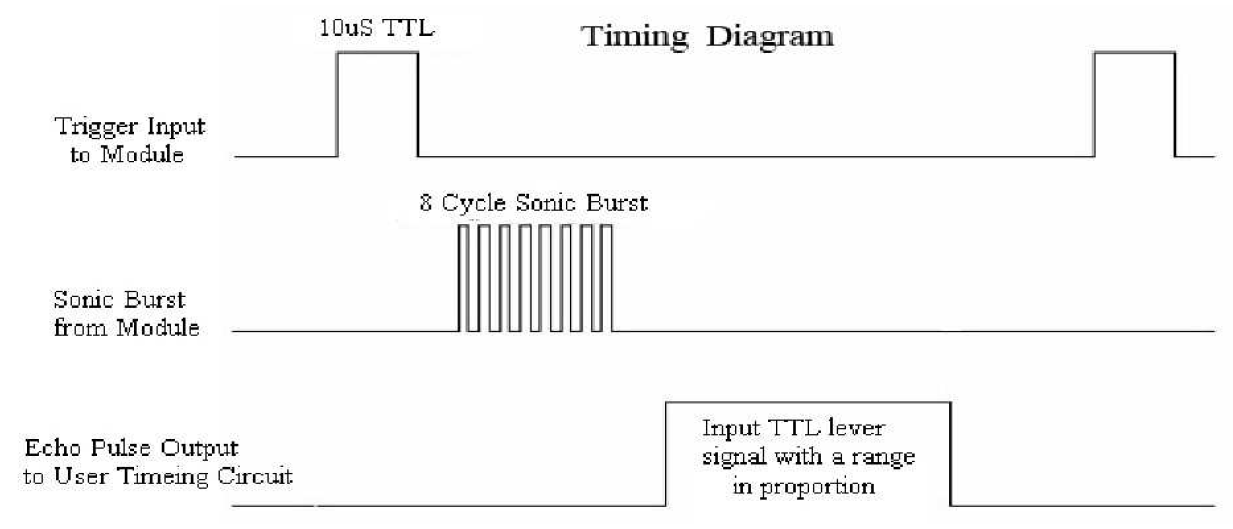
\includegraphics[width=\linewidth]{0_Filer/Figuer/5_HW_Design/HC-SR04_Ultra_Sonic_Timing_Diagram.PNG}
    \caption{HC-SR04 timing diagram}
    \label{fig:HWD_SR04_timing}
\end{figure}

\subsubsection{Bevægelses sensor (PIR)}

Den valgte PIR sensor til projektet er af typen HC-SR501. Sensoren har 3 ben -  VCC, GND og et digitalt output ben. HC-SR501 skal have en forsyningsspænding på mellem 5 og 20 VDC og bruger 65mA. Det digitale output er med TTL standard, hvor High = 3,3V og Low = 0V. HC-SR501 har en justerbar forsinkelse på mellem 0,3 og 5 min. Samt mulighed for at justere max-sensor range fra 3 til 7 m. Både delay og range stilles ved hjælp af hver deres potentiometer.

Ved opstart af modulet vil modulet udsende TTL high 0-3 gange i løbet af det første minut, og derefter gå i standby. Herefter er modulet klar.

Der er mulighed for at sætte sensoren op i to modes ved hjælp af en jumper. Non-repeatable trigger og Repeatable trigger.

Non-repeatable trigger: Når sensoren aktiveres går output benet høj i det interval, der er indstillet med delayet, derefter går benet lavt igen. Benet bliver ikke holdt højt ved gentagen bevægelse, men kan først trigges igen, når det er gået lavt.

Repeatable trigger: Når sensoren aktiveres går output benet højt, og så længe der fortsat er bevægelse vil benet forblive højt. Når bevægelse ophører, vil benet forblive højt til delayet er slut og derefter gå lavt.

\begin{figure}[H]
\centering
\begin{minipage}{.6\textwidth}
  \centering
    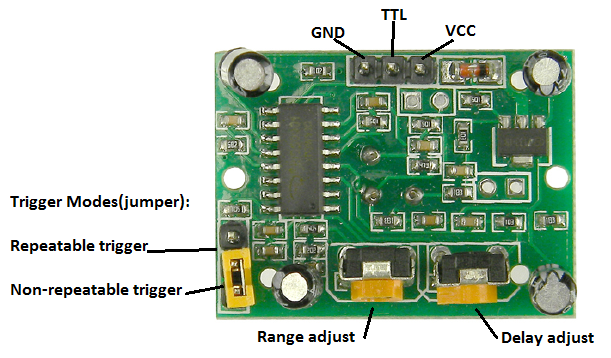
\includegraphics[width=\linewidth]{0_Filer/Figuer/5_HW_Design/HC-SR501_PIR_Motion_Detector_image.png}
    \caption{HC-SR501 PIR sensor}
    \label{fig:HWD_SR501}
\end{minipage}%
\begin{minipage}{.4\textwidth}
  \centering
    \begin{tabular}{ | l | l | }
        \hline
        \textbf{PSoC} & \textbf{HC-SR501} \\ \hline
        GND & GND \\ \hline
        5 V & Vcc \\ \hline
        P2\textunderscore{}0 & TTL \\
        \hline
    \end{tabular}
    \caption{Portforbindelser}
    \label{fig:HWD_PIR_ports}
\end{minipage}
\end{figure}

\subsubsection{5V Stepper motor}

\begin{figure}[H]
\centering
\begin{minipage}{.5\textwidth}
  \centering
  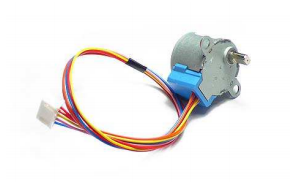
\includegraphics[width=\linewidth]{0_Filer/Figuer/5_HW_Design/Stepper_motor.png}
  \caption{5V stepper motor}
  \label{fig:HWD_Stepper_Motor}
\end{minipage}%
\begin{minipage}{.5\textwidth}
  \centering
  
\includegraphics[width=\linewidth]{0_Filer/Figuer/5_HW_Design/Motor_diagram.png}
  \caption{Intern forbindelse i motoren}
  \label{fig:HWD_Stepper_Diagram}
\end{minipage}
\end{figure}

Til styring af X,Y og Z retning benyttes en 5V stepper motor af typen 28BYJ-48. Motoren er et oplagt valg, siden den er let tilgængelig på embedded stock, og da den lever op til de krav, som er til systemet. Yderligere er 28BYJ-48-motoren mere kompatibel med det størrelsesforhold prototypen bygges i. Der udover er motorens præcision fordelagtig for projektet, da den har en gearing på 64x48. Dvs. at der er 3072 steps pr. omgang, som gør at lampen kan positioneres meget præcist.

\begin{figure}[H] \centering
    \fbox{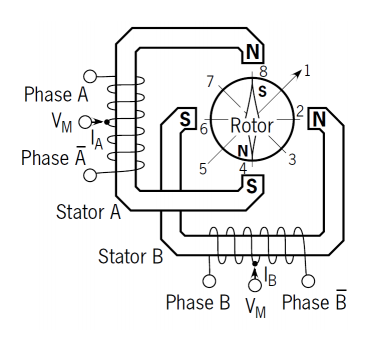
\includegraphics[width=.6\textwidth]{0_Filer/Figuer/5_HW_Design/Bipolar_motor_diagram.png}}
    \caption{Stepper motor}
    \label{fig:HWD_Bipolar_Stepper_Motor}
\end{figure}

Forklaringen herunder tager udgangspunkt i Stator A.
\newline Motoren består af 2 statorer med en nord- og en sydpol. Hver stator har viklinger med to ende tilslutninger, phase A og phase A’, mellem de to ende tilslutninger tilsluttes en 5VDC spænding(Vm). Se figur \ref{fig:HWD_Bipolar_Stepper_Motor}.
Ved at tilslutte phase A til stel, vil strømmen bevæge sig fra Vm til phase A gennem viklingerne, denne bevægelse vil danne et magnetfelt, hvor nord og sydpolen er som på figur \ref{fig:HWD_Bipolar_Stepper_Motor}. Ved tilslutning af phase A’ vil strømmen bevæge sig i modsat retning og de to poler vil bytte plads. Dette gælder også for stator B. Når polerne skifter vil rotorens poler i motoren blive henholdsvis tiltrukket og afvist af statorens poler.

\subsubsection{Micro switch}

\begin{figure}[H]
\centering
\begin{minipage}{.5\textwidth}
  \centering
  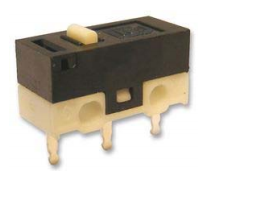
\includegraphics[width=\linewidth]{0_Filer/Figuer/5_HW_Design/Micro_switch.png}
  \caption{Micro Switch (DM1-01P-30-3)}
  \label{fig:HWD_Micro_switch}
\end{minipage}%
\begin{minipage}{.5\textwidth}
  \centering
  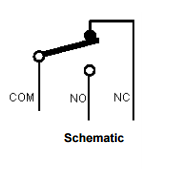
\includegraphics[width=\linewidth]{0_Filer/Figuer/5_HW_Design/Micro_switch_diagram.png}
  \caption{Forbindelses diagram af micro switch}
  \label{fig:HWD_Micro_Diagram}
\end{minipage}
\end{figure}

Til håndtering af ende stop og kalibrering af X-,Y- og Z-retninger, installeres 5 micro switches(DM1-01P-30-3). To switches placeres i enderne på X-skinnen, to på Y-skinnens ender og en ved lampens top-position. Ved aktivering af en af micro switches sættes en port høj på den tilhørende PSoC4, som vil stoppe den bevægelse der nu er nået enden.
Micro switchen forbindes som en NO(normaly open) switch med 5V på COM benet og NO benet forbundet til PSoC4. Se \ref{fig:HWD_Micro_Diagram}.
Iflg. Databladet er micro switchen rated 5V DC og 30mA.

\subsubsection{Strømforbrug}

En enkelt motor bruger 150 mA, når den ikke drejer. Strømforbruget falder når motoren kører. PSoC-XY kommer derfor til at levere mest strøm, da den forsyner 4 motorer, altså 4x 150 mA, og dermed 600 mA hvilket ikke er noget problem for en PSoC. PSoC-Sensor vil levere næstmest strøm i størrelsesordenen 260 mA, beregnet samlet ud fra de forskellige sensorer og LED’er som skal drives af PSoC’en. PSoC-Z levere kun strøm til én motor, hvilket bliver 150 mA.

\subsubsection{Motorstyring}

Et styringsprint er lavet til positionering af vores stepper-motorer. Dette er valgt for at lave en samlet printboks bestående af prints og PSoC’s i vores system. På denne måde kan diverse ledninger, der ellers ville ligge rodet oven i hinanden, blive pakket kompakt i en mere æstetisk behagelig kasse.

\begin{figure}[H] \centering
    \fbox{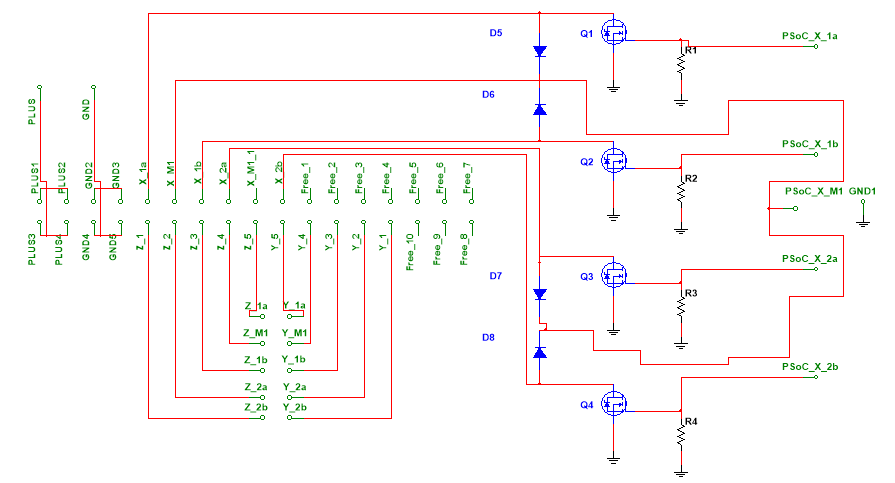
\includegraphics[width=\textwidth]{0_Filer/Figuer/5_HW_Design/X-Diagrammet.PNG}}
    \caption{Styringsprint til X-akse og 34-leder}
    \label{fig:HWD_Styringsprint_til_x_print}
\end{figure}

Kommunikationen går fra de styrende prints gennem et 34-lederkabel og ud til aktuatorerne. På Figur \ref{fig:HWD_Styringsprint_til_x_print} ses et diagram for udlægget af 34-lederkablet. I forsyningskredsløbet sendes der et input ind fra den styrende PSoC, som da bliver forstærket igennem en MosFet. Herefter bliver det sendt ud på 34-lederkablet og går op i et splitterprint i vognene på X- og Y-aksen. Fra disse splitterprints, går signalet direkte ud til steppermotorerne. 


\textbf{Styringskode:}\newline 
Styringen af systemets motorer foregår i tildelte PSoCs. Hver bevægelsesretning har en PSoC tildelt som styre retning og antal trin motoren skal køre. Aktivering af motorerne kan initieres i PSoC'en på to måder. Manual-mode og Automatic-mode. Der skiftes mellem disse to modes ved tryk på switch på PSoC. Nuværende mode indikeres gennem farven på LED.

\textbf{Manual-Mode:} Indikeres med farven rød på LED på PSoC.\newline 
Når LED’en på PSoC’en lyser rød, er I2C kommunikation med Master-PSoC slået fra, og Capsense slideren på PSoC’en er slået til. 
Slideren er delt op i fire felter, fra 0 til 128, til manuel bevægelse af motorerne.  Felt 1 er alle værdier under 32. felt 2 er værdier mellem 32 og 64. felt 3 er værdier mellem 64 og 96. felt 4 er værdier over 96.
Disse fire felter styrer hver deres bevægelse af motorerne. Felt 1 er Y-motorerne i den ene retning, felt 2 er Y-motorerne i modsat retning af Felt 1. Felt 3 er X-motorerne tilsvarende i den ene retning, og Felt 4 er modsat retning af Felt 3. 
For at aktivere disse retningskørsler trykkes der på et givent felt på Capsense-slideren, og fingeren holdes i kontakt med dette felt, så længe kørsel med motorerne ønskes. Motorerne stoppes når kontakt med felt afbrydes.\newline 

Oversigt over felterne:\newline
\verb+Kør_X_frem();+       mellem 64 og 96 på touch-sense\newline
\verb+Kør_X_tilbage();+      over 96 på touch-sense\newline
\verb+Kør_Y_frem();+	   mellem 64 og 32 på touch-sense\newline
\verb+Kør_Y_tilbage();+	     under 32 på touch-sense\newline

\textbf{Automatic-Mode:} Indikeres med farven grøn på LED på PSoC.\newline 
Når LED’en på PSoC’en lyser grøn, er Capsense slideren på PSoC’en slået fra, og I2C kommunikation med Master-PSoC er slået til. 
Ved Automatic-mode modtager PSoC’en til styring af XY-retningen en kommandokode fra PSoCMaster. Denne kommandokode kommer via I2C gennem  P4[0] til SCL og P4[1] til SDA på PSoC-XY.
Kommandokoden identificeres til et funktionskald og en parameter. For at køre med motorerne, kræver det at det første funktionskald, der bliver givet er kalibrer\textunderscore{}system. 

\textbf{Styringskode opbygning:}\newline
For overskuelighed er koden delt op i nogle header- og source filer se \ref{fig:XYhs} 

% XY header/source filer
\begin{figure}[H] \centering
    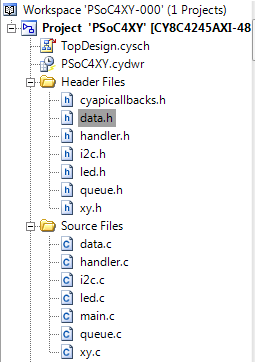
\includegraphics[width=0.3\linewidth]{0_Filer/Figuer/5_HW_Design/HeaderSourceOversigt.PNG}
    \caption{XY header/source filer}
    \label{fig:XYhs}
\end{figure}

\verb+cyapicallbacks:+\newline
Denne del er koden sørger for at når der kommer en kommando på I2C, kalder den et interupt, der stopper programmet og ser på hvilken kommando der er kommet. Efter følgene hopper den tilbage hvor den kom til i programmet og fortsætter med de eventuelt nye parametre der er kommet. \newline
\verb+data:+\newline

\verb+handler:+\newline
\verb+i2c:+\newline
\verb+led:+\newline
\verb+queue:+\newline
\verb+xy:+\newline
\verb+main:+\newline

%Venter med resten for at se hvad jeppe skriver

\textbf{Kalibrer\textunderscore{}system()}\newline 
Dette funktionskald aktiverer X-motorerne i den ene retning. Når retningens grænse er nået, vil en fysisk afbryder blive aktiveret og herved leverer besked til PSoC-XY om at den nedre grænse er nået. Herefter vil X-motorerne køre i den anden retning til de rammer den øvre grænse hvor endnu en afbryder bliver aktiveret. \newline 
De steps motoren tager imellem den nedre og øvre grænse bliver gemt i en integer variabel kaldet X-max. Motorens nuværende position ved den øvre grænse gemmes i en integer variabel kaldet X-position som bliver sat til 0. \newline 
Når X-max og X-position er sat, aktiveres Y-motorerne i den ene retning. Når retningens grænse er nået, vil en fysisk afbryder blive aktiveret og herved leverer besked til PSoC-XY om at den nedre grænse er nået. Herefter vil Y-motorerne køre i den anden retning til de rammer den øvre grænse hvor endnu en afbryder bliver aktiveret. \newline 
Her bliver antal steps Y-motorerne har kørt gemt i en integer variabel kaldet Y-max, og motorens nuværende position bliver gemt i en integer variabel kaldet Y-position som sættes til 0. 
Hermed er skinnernes længde målt ud, lampens position er sat og systemet er nu kalibreret.   \newline  
\textbf{Get\textunderscore{}X()}\newline 
Denne funktion returnerer motorens position fra 0 til 255 fordelt ud på X-max værdien.  \newline 
\textbf{Set\textunderscore{}X()}\newline 
Denne funktion aktivere X-motorerne. Funktionen giver en parameter fra 0 til 255. Denne parameter bruges til at sætte den ønskede position som motorerne skal køre til. Hvis ønskede position er det samme som nuværende position, køres der ikke med motorerne. Alt efter hvilken position der bliverønsket fra PSoC-Master, regner PSoC-XY selv ud hvilken retning motorerne skal køre for at opnå den ønskede position. \newline  
\textbf{Get\textunderscore{}Y()}\newline 
Denne funktion returnerer motorens position fra 0 til 255 fordelt ud på Y-max værdien.  \newline 
\textbf{Set\textunderscore{}Y()}\newline 
Denne funktion aktivere Y-motorerne. Funktionen giver en parameter fra 0 til 255. Denne parameter bruges til at sætte den ønskede position som motorerne skal køre til. Hvis ønskede position er det samme som nuværende position, køres der ikke med motorerne. Alt efter hvilken position der bliver ønsket fra PSoC-Master, regner PSoC-XY selv ud hvilken retning motorerne skal køre for at opnå den ønskede position.  \newline 

\clearpage
\clearpage

% 6. Software design
% 6. Software design
\chapter{Software design}

% 6.1 Design
% 6.1 Design
\section{Design}

% 6.1.1 Dataprotokol
% 6.1.1 Dataprotokol
\subsection{Dataprotokol}

\subsubsection{Kommandoer}

Igennem hele systemet benyttes os af 8-bit hex kommandoer jf. tabel \ref{tab:kommandoTabel}

\begin{table}[H]
    \centering
    \begin{tabular}{|c|l|l|l|l|l|l|}
    \hline
        \textbf{Hex} &
        \textbf{Kommando} &
        \textbf{Parameter} &
        \textbf{Retur værdi} &
        \textbf{Fra enhed} &
        \textbf{Til enhed} &
        \textbf{Interface}\\
    \hline
        0x11 &
        setX &
        unsigned char &
        ingen &
        DevKit &
        PSoC Master &
        SPI \\
    \hline
        0x12 &
        setY &
        unsigned char &
        ingen &
        DevKit &
        PSoC Master &
        SPI \\
    \hline
        0x13 &
        setZ &
        unsigned char &
        ingen &
        DevKit &
        PSoC Master &
        SPI \\
    \hline
        0x21 &
        setR &
        unsigned char &
        ingen &
        DevKit &
        PSoC Master &
        SPI \\
    \hline
        0x22 &
        setG &
        unsigned char &
        ingen &
        DevKit &
        PSoC Master &
        SPI \\
    \hline
        0x23 &
        setB &
        unsigned char &
        ingen &
        DevKit &
        PSoC Master &
        SPI \\
    \hline
        0x31 &
        getX &
        ingen &
        unsigned char* &
        DevKit &
        PSoC Master &
        SPI \\
    \hline
        0x32 &
        getY &
        ingen &
        unsigned char* &
        DevKit &
        PSoC Master &
        SPI \\
    \hline
        0x33 &
        getZ &
        ingen &
        unsigned char* &
        DevKit &
        PSoC Master &
        SPI \\
    \hline
        0x41 &
        getR &
        ingen &
        unsigned char* &
        DevKit &
        PSoC Master &
        SPI \\
    \hline
        0x62 &
        getG &
        ingen &
        unsigned char* &
        DevKit &
        PSoC Master &
        SPI \\
    \hline
        0x43 &
        getB &
        ingen &
        unsigned char* &
        DevKit &
        PSoC Master &
        SPI \\
    \hline
        0x50 &
        cmdCalibrate &
        ingen &
        ingen &
        DevKit &
        PSoC Master &
        SPI \\
    \hline
        0x51 &
        cmdStatus &
        ingen &
        unsigned char* &
        DevKit &
        PSoC Master &
        SPI \\
    \hline
        0x60 &
        cmdDistanceAlert &
        ingen &
        ingen &
        PSoC Sensor &
        PSoC Master &
        I2C \\
    \hline
        0x70 &
        cmdCalibrate &
        ingen &
        ingen &
        PSoC Master &
        PSoC XY &
        I2C \\
    \hline
        0x71 &
        setX &
        unsigned char &
        ingen &
        PSoC Master &
        PSoC XY &
        I2C \\
    \hline
        0x72 &
        setY &
        unsigned char &
        ingen &
        PSoC Master &
        PSoC XY &
        I2C \\
    \hline
        0x75 &
        getX &
        ingen &
        unsigned char* &
        PSoC Master &
        PSoC XY &
        I2C \\
    \hline
        0x76 &
        getY &
        ingen &
        unsigned char* &
        PSoC Master &
        PSoC XY &
        I2C \\
    \hline
        0x77 &
        getXMax &
        ingen &
        unsigned char* &
        PSoC Master &
        PSoC XY &
        I2C \\
    \hline
        0x78 &
        getYMax &
        ingen &
        unsigned char* &
        PSoC Master &
        PSoC XY &
        I2C \\
    \hline
        0x80 &
        cmdCalibrate &
        ingen &
        ingen &
        PSoC Master &
        PSoC Z &
        I2C \\
    \hline
        0x81 &
        setZ &
        unsigned char &
        ingen &
        PSoC Master &
        PSoC Z &
        I2C \\
    \hline
        0x85 &
        getZ &
        ingen &
        unsigned char* &
        PSoC Master &
        PSoC Z &
        I2C \\
    \hline
        0x86 &
        getZMax &
        ingen &
        unsigned char* &
        PSoC Master &
        PSoC Z &
        I2C \\
    \hline
        0x89 &
        cmdDistanceAlert &
        ingen &
        ingen &
        PSoC Master &
        PSoC Z &
        I2C \\
    \hline
        0x90 &
        cmdCalibrate &
        ingen &
        ingen &
        PSoC Master &
        PSoC Sensor &
        I2C \\
    \hline
        0x91 &
        setR &
        unsigned char &
        ingen &
        PSoC Master &
        PSoC Sensor &
        I2C \\
    \hline
        0x92 &
        setG &
        unsigned char &
        ingen &
        PSoC Master &
        PSoC Sensor &
        I2C \\
    \hline
        0x93 &
        setB &
        unsigned char &
        ingen &
        PSoC Master &
        PSoC Sensor &
        I2C \\
    \hline
        0x94 &
        setLumen &
        unsigned char &
        ingen &
        PSoC Master &
        PSoC Sensor &
        I2C \\
    \hline
        0x95 &
        getPower &
        ingen &
        unsigned char* &
        PSoC Master &
        PSoC Sensor &
        I2C \\
    \hline
        0x96 &
        getR &
        ingen &
        unsigned char* &
        PSoC Master &
        PSoC Sensor &
        I2C \\
    \hline
        0x97 &
        getG &
        ingen &
        unsigned char* &
        PSoC Master &
        PSoC Sensor &
        I2C \\
    \hline
        0x98 &
        getB &
        ingen &
        unsigned char* &
        PSoC Master &
        PSoC Sensor &
        I2C \\
    \hline
        0x99 &
        getLumen &
        ingen &
        unsigned char* &
        PSoC Master &
        PSoC Sensor &
        I2C \\
    \hline
    \end{tabular}
    \caption{Kommandoer tabel}
    \label{tab:kommandoTabel}
\end{table}
\clearpage

% 6.1.2 Applikationsmodeller
% 6.1.2 Applikationsmodeller
\subsection{Applikationsmodeller}

Selve designet af softwaren bygger på de følgende applikationsmodeller. Her laves der sekvens- og klassediagrammer over hver del af systemet samt klassebeskrivelser, hvor funktionen for de enkelte metoder beskrives.

% 6.1.2.1 DevKit8000
\subsubsection{DevKit8000}

Applikationsmodel for UC1: Kalibrer system.

\begin{figure}[H] \centering
    \fbox{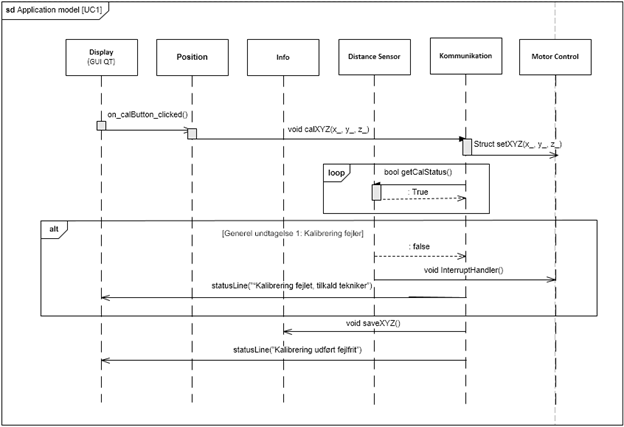
\includegraphics[width=0.95\textwidth]{0_Filer/Figuer/uc1App.png}}
    \caption{Applikationsmodel med udgangspunkt i UC1}
    \label{fig:uc1App}
\end{figure}

\begin{figure}[H] \centering
    \fbox{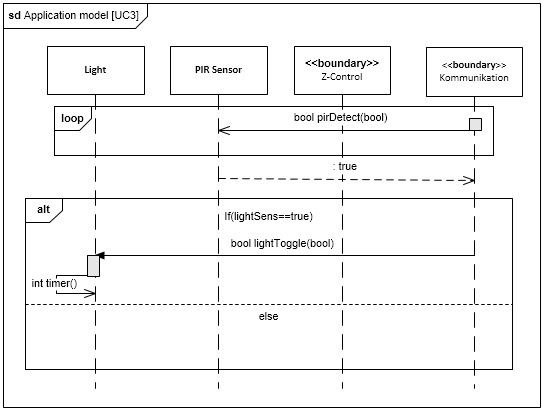
\includegraphics[width=0.95\textwidth]{0_Filer/Figuer/uc3App.png}}
    \caption{Applikationsmodel med udgangspunkt i UC3}
    \label{fig:uc3App}
\end{figure}


% 6.1.2.2 PSoC Master
\subsubsection{PSoC Master}

Applikationsmodeller for PSoC Master.

\begin{figure}[H] \centering
    \fbox{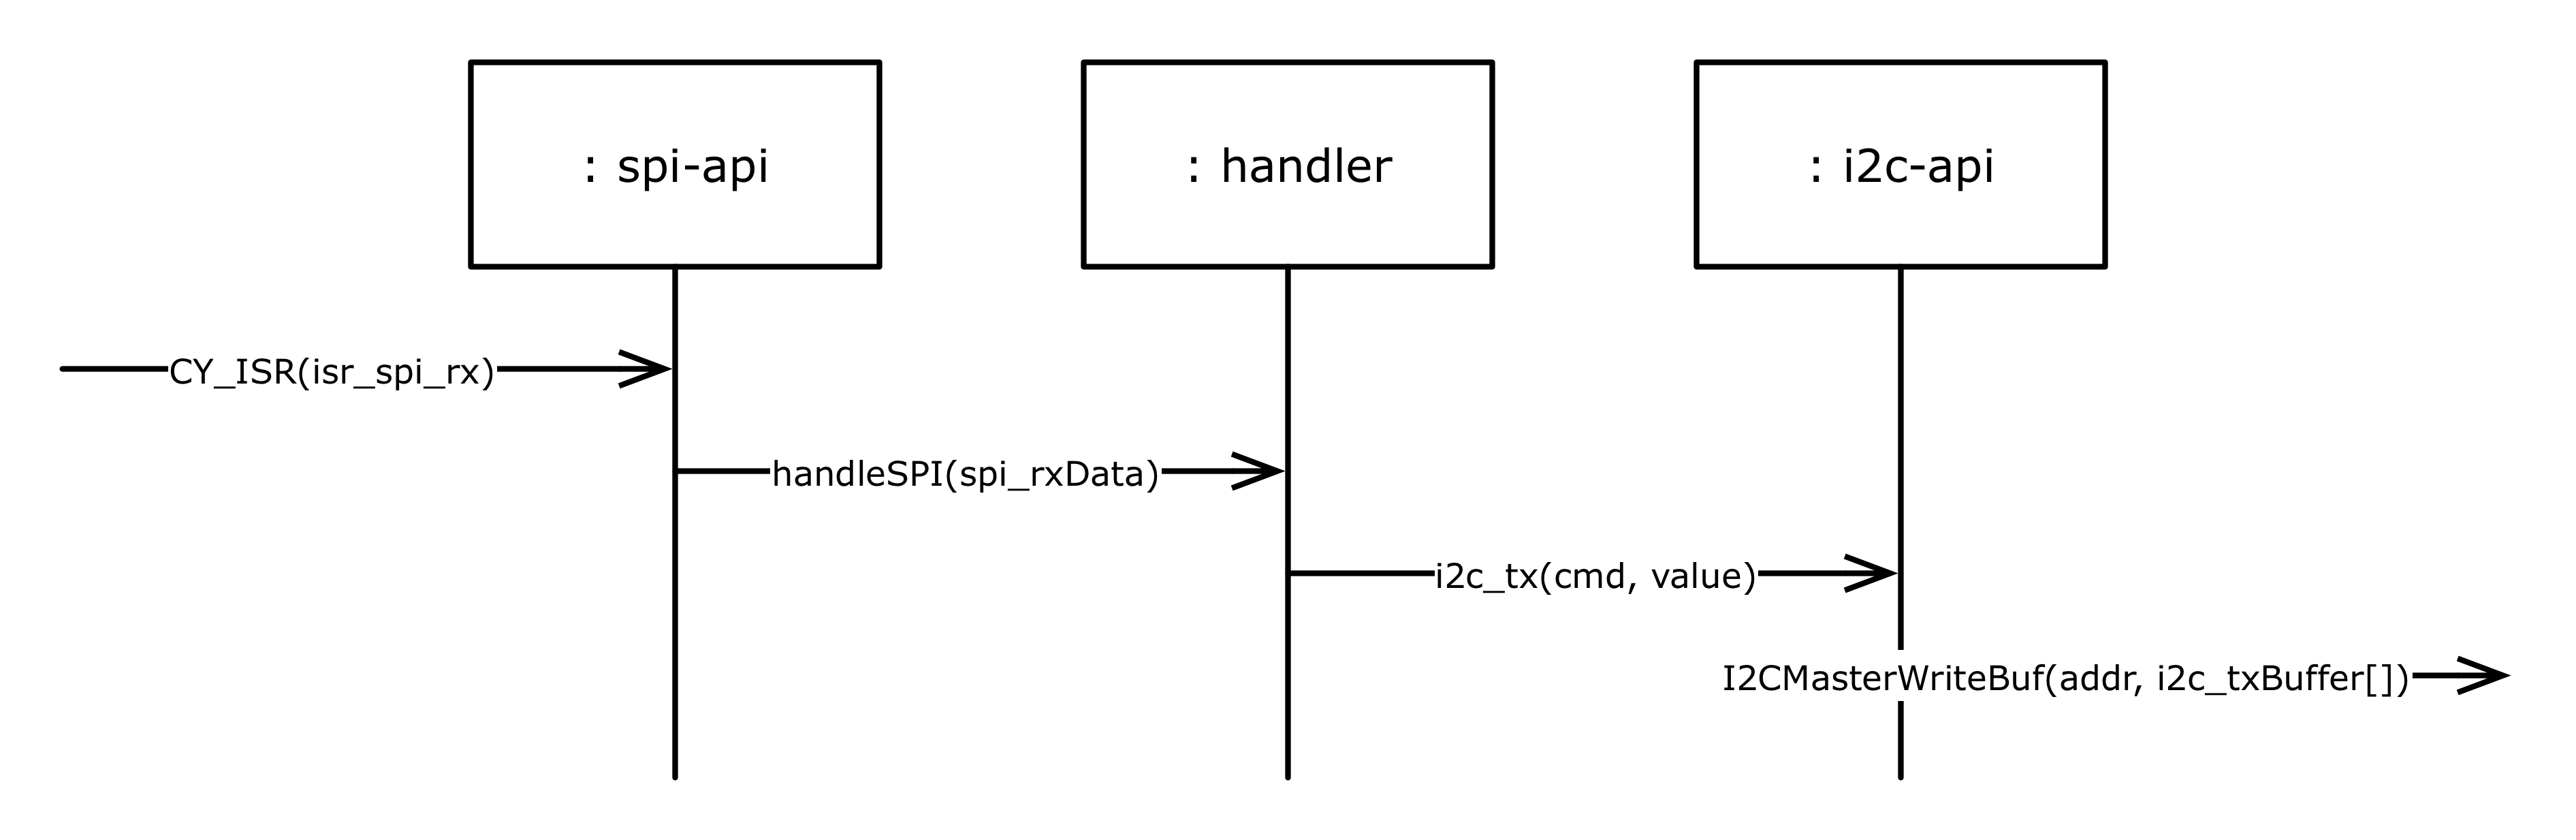
\includegraphics[width=0.95\textwidth]{0_Filer/Figuer/SPItoI2C.png}}
    \caption{Sekvensdiagram for "set" kommando via PSoC Master}
    \label{fig:sekvensdiagram_psoc_master_set}
\end{figure}

\begin{figure}[H] \centering
    \fbox{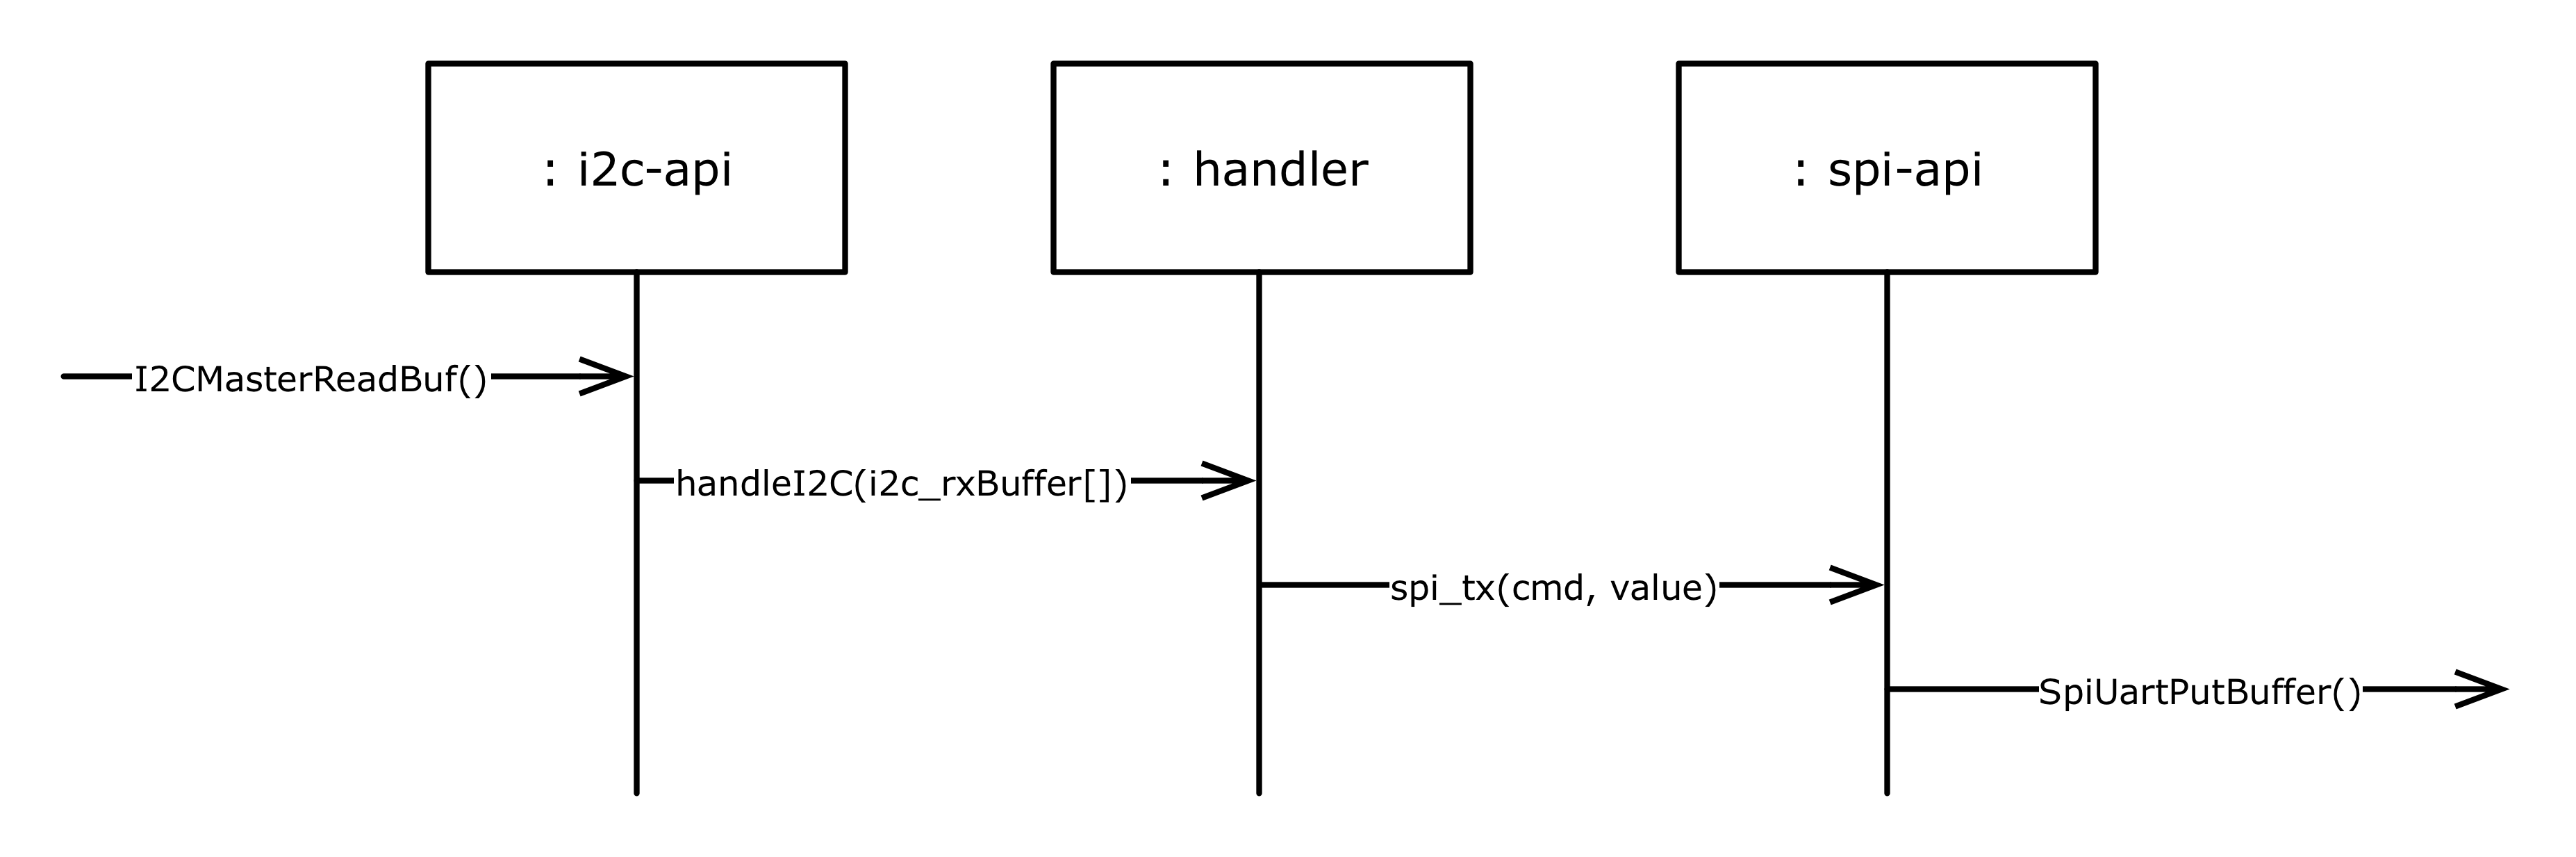
\includegraphics[width=0.95\textwidth]{0_Filer/Figuer/I2CtoSPI.png}}
    \caption{Sekvensdiagram for "get" kommando via PSoC Master}
    \label{fig:sekvensdiagram_psoc_master_get}
\end{figure}

% 6.1.2.3 Klassebeskrivelser
\subsubsection{Klassebeskrivelser PSoC Master}

Her følger klassebeskrivelser for de udledte klasser fra applikationsmodellerne.
% 6.1.2.3 Klassebeskrivelser PSoC Master

% spi-api
\begin{table}[H]
    \centering
    \begin{tabular}{|l|}
    \hline
    \multicolumn{1}{|c|}{<<boundary>>} \\
    \multicolumn{1}{|c|}{\textbf{SPI-API}} \\
    \hline
    - uint16 spi\_rxData \\
    - uint16 spi\_txData \\
    \hline
    + spi\_init() :void \\
    + spi\_tx(uint16) : void \\
    + CY\_ISR(isr\_spi\_rx) \\
    \hline
    \end{tabular}
    \caption{Klassen SPI-API på PSoC-Master}
    \label{tab:classSpiApiPSoCMaster}
\end{table}

{\centering\textbf{spi-api (PSoC Master)}\par}

\begin{labeling}{Attributter:}
\item[Ansvar:] At håndtere spi kommuniaktionen mellem DevKit og PSoC Master.
\item[Attributter:] uint16 spi\_rxData \\
uint16 spi\_txData
\end{labeling}

\begin{labeling}{Beskrivelse:}
\item[void spi\_init()]
\item[Parametre:] Ingen.
\item [Returværdi:] Ingen.
\item [Beskrivelse:] Initialsere SPI komponentet på PSoC Master.
\end{labeling}

\begin{labeling}{Beskrivelse:}
\item[void spi\_tx(uint16)]
\item[Parametre:] Modtager en unsigned int 16.
\item [Returværdi:] Ingen.
\item [Beskrivelse:] Metoden modtager en unsigned int på 16-bit, som den lægger klar til anvendelse via SPI kommuniaktionen til DevKit ved næste ledige bus tid.
\end{labeling}

\begin{labeling}{Beskrivelse:}
\item[CY\_ISR(isr\_spi\_rx)]
\item[Parametre:] Navnet på isr funktionen.
\item [Returværdi:] Ingen.
\item [Beskrivelse:] Metoden opretter en isr som klades automatisk, når der bliver sendt data til PSoC Master via spi kommuniaktionen.
\end{labeling}

% handler
\begin{table}[H]
    \centering
    \begin{tabular}{|l|}
    \hline
    \multicolumn{1}{|c|}{<<controler>>} \\
    \multicolumn{1}{|c|}{\textbf{handler}} \\
    \hline
    \\
    \hline
    + handleSPI(uint8, uint16) : void \\
    + handleI2C(uint8, uint16) : void \\
    \hline
    \end{tabular}
    \caption{Klassen handler på PSoC-Master}
    \label{tab:classHandlerPSoCMaster}
\end{table}

{\centering\textbf{handler (PSoC-Master)}\par}

\begin{labeling}{Attributter:}
\item[Ansvar:] At håndtere alt data flow på PSoC Master.
\item[Attributter:] ingen.
\end{labeling}

\begin{labeling}{Beskrivelse:}
\item[void handleSPI(uint8, uint16)]
\item[Parametre:] Modtager en unsigned int 8 og en unsigned int 16.
\item [Returværdi:] Ingen.
\item [Beskrivelse:] Metoden modtager en unsigned int på 8-bit, som indholder en kommandoen, der håndteres og en tilhørende unsigned int på 16-bit, som indholder en værdi.
\end{labeling}

\begin{labeling}{Beskrivelse:}
\item[void handleI2C()]
\item[Parametre:]Modtager en unsigned int 8 og en unsigned int 16.
\item [Returværdi:] Ingen.
\item [Beskrivelse:] Metoden modtager en unsigned int på 8-bit som indholder en kommandon som håndteres og en tilhørende unsigned int på 16-bit som indholder en værdi.
\end{labeling}

% I2C-API
\begin{table}[H]
    \centering
    \begin{tabular}{|l|}
    \hline
    \multicolumn{1}{|c|}{<<boundary>>} \\
    \multicolumn{1}{|c|}{\textbf{I2C-API}} \\
    \hline
    - uint8 i2c\_txBuffer[] \\
    - uint8 i2c\_txBuffer[] \\
    \hline
    + i2c\_init() : void \\
    + i2c\_tx() : void \\
    + i2c\_rx() : void \\
    \hline
    \end{tabular}
    \caption{Klassen I2C-API på PSoC Master}
    \label{tab:classI2cApiPSoCMaster}
\end{table}

{\centering\textbf{I2C-API (PSoC Master)}\par}

\begin{labeling}{Attributter:}
\item[Ansvar:] At håndtere I2C kommuniaktionen mellem PSoC-Master og PSoC-XY, PSoC-Z og PSoC-Sensor.
\item[Attributter:] uint8 i2c\_txBuffer[]\\
uint8 i2c\_txBuffer[]
\end{labeling}

\begin{labeling}{Beskrivelse:}
\item[void i2c\_init()]
\item[Parametre:] Ingen.
\item [Returværdi:] Ingen.
\item [Beskrivelse:] Initialsere I2C komponentet på PSoC Master.
\end{labeling}

\begin{labeling}{Beskrivelse:}
\item[void i2c\_tx(uint16)]
\item[Parametre:] Modtager en unsigned int 16.
\item [Returværdi:] Ingen.
\item [Beskrivelse:] Metoden modtager en unsigned int på 16-bit, som den lægger klar til anvendelse via I2C kommuniaktionen.
\end{labeling}

\begin{labeling}{Beskrivelse:}
\item[void i2c\_rx(uint16)]
\item[Parametre:] Modtager en unsigned int 16.
\item [Returværdi:] Ingen.
\item [Beskrivelse:] Metoden modtager en unsigned int på 16-bit, som den lægger klar til anvendelse via I2C kommuniaktionen.
\end{labeling}



\subsubsection{PSoC-Sensor arkitektur og implementering}

På TopDesign niveau består PSoC-Sensor af 7 blokke:
\begin{itemize}
	\item Afstandssensor
	\item PIR sensor
    \item Lumen sensor
	\item LED PWM
	\item Intern kommunikation
	\item Main lop metronom
	\item Debug
\end{itemize}

For at aflæse afstandssensoren skal vi kunne måle hvor længe en pin bliver holdt høj, med en præcision på et par mikrosekunder (1 cm svare til 58 us). Derfor har vi sat en timer op med en 1 MHz clock, der starter med at tælle på rising edge af det signal der skal måles, og derefter stopper, gemmer tællerværdien og starter en interrupt på falling edge. 

Denne blok har desuden tre ekstra pins: DistTrigger, DistReset, og DistInterruptPin. DistTrigger bruges til at starte målingen - sensoren skal have en 10 us puls som input før den starter. DistReset bruges til at resette timeren mellem målingerne, da den ellers blot fortsætter med at tælle derfra hvor den kom til. Til sidst bruges DistInterruptPin til at sende et signal direkte til PSoC-Z når afstandssensoren måler at vi er kommet for tæt på en underliggende forhindring.

PIR sensor blokken er noget simplere: Sensoren holder et output højt når den detekterer bevægelse og lavt ellers, så der behøves blot en pin til at aflæse det signal.

Lyssensoren kommunikere over I2C, så her behøves kun et I2C Master modul.

De tre LEDs styres med PWM, og hver farve (rød, grøn, blå) har sit eget PWM modul. De deler dog alle tre clock med afstandssensor-timeren. Dette er valgt fordi PSoC4 maksimalt understøtter fire brugerdefinerede clocks, så når forskellige komponenter kan sættes til at virke med samme clock-frekvens, er der ingen grund til at bruge flere resourcer end nødvendigt.

Den interne kommunikation mellem PSoCs foregår med I2C protokollen, men i det her tilfælde er Sensor-PSoC en slave.

Den næstsidste blok er Metronomen. Den indeholder en timer der er sat til at lave et interrupt hvert halve sekund. De interrupts bliver så brugt i hovedprogrammet til at aktiverer sensoraflæsninger og andre periodiske events. Denne timer har sin egen clock (200 Hz), da det gjorde designet nemmere og lod os holde timeren på 8 bits, hvilket spare andre resourcer i PSoC'en.

Den sidste blok er Debug. Den indeholder et UART modul, men da de to I2C moduler optager alle de dedikerede hardware kommunikationsblokke, så der bliver her brugt et software modul der kun understøter transmit.

{\centering\textbf{PSoC-Sensor implementering}\par}

I softwaren findes der disse filer:
\begin{itemize}
	\item SensorData
	\item CircularMean
	\item i2c
	\item queue
	\item handler
	\item LumenSensor
	\item lux
	\item main
\end{itemize}

\textbf{SensorData} har en struct der indeholder alle de globale sensor data og instillinger systemet bruger, samt en init funktion der sætter værdierne til noget fornuftigt under opstart.

\textbf{CircularMean} er datastruktur der kun kan modtage integer data og returnerer en gennemsnitlig værdi for de sidste X indsatte værdier. Så den er lidt dårligt navngivet og burde have heddet CircularAverage. Den er implementeret med et array der bliver indekseret fortløbende indtil enden bliver nået, hvorefter skrive-pointeren bliver nulstillet og de ældste værdier begynder at blive overskrevet.

\textbf{i2c} og \textbf{queue} er de moduler der håndterer I2C kommunikationen. Disse moduler er nærmere beskrævet i TODO: INSERT-REFERENCE

Modulet \textbf{handler} håndterer PSoC-Sensors opførsel når den modtager I2C kommandoer fra PSoC-Master. Den er implementeret med en stor switch, med en case for hver kommando PSoC-Sensor kan modtage og håndterer. Desuden har modulet en debug funktion, hvor man ved at aktiverer en \#define kan få alle modtagne kommandoer udskrevet på debug uart forbindelsen.

\textbf{LumenSensor} er det software modul der håndterer I2C kommunikationen med lyssensoren. Dette har fået sit eget modul da en enkelt aflæsning af sensoren består af at skrive en byte til sensoren, læse to bytes fra sensoren, og derefter skrive en og læse to bytes igen. Denne kommunikation bruger \texttt{NO\_STOP} og \texttt{REPEAT\_START} flagende, hvilket gør at alle fire dataoverførsler teknisk set foregår i en I2C kommunikation. Dette betyder ikke noget her da der kun er en master og en slave på linjen, men i et større system vil det forhindre en anden master i at tage linjen i det splitsekund hvor den bliver frigivet. Derudover spare man også omkring 3 bits på linjen på de udeblivende stop.

\textbf{lux} modulet er ikke noget vi har skrevet selv. De målinger lyssensoren giver bør køres gennem en formel der som resultat giver et rimeligt tal for den mængde synligt lys sensoren kan se, i måleenheden lux. Denne formel er beskrevet i sensorens datablad, og databladet indeholder desuden en færtig C-funktion der kan udføre beregningen hurtigt og effektivt på en mikroprocessor. Det er denne C-funktion vi har kopieret over i lux modulet.

Sidst men ikke mindst er der \textbf{main}. Den indeholder den overordnede kontrolstruktur i PSoC-Sensor, der bestemmer hvornår alt andet skal køres. Som beskrevet ovenfor i TopDesign, så er hjertet Metronom timeren der giver et taktslag hver halve sekund. For hvert taktslag bliver en række tællere talt op og tjekket for overløb. Hver tæller der løber over bliver nulstillet og hæver et flag. De flag bliver så tjekket i hovedløkken og den tilhørende kode bliver udført.

Alt i alt giver denne opbygning at der kan defineres periodiske events med individuelle perioder (med en opløsning på 0.5 sekunder). Det giver den fordel at vi kan have en hoved-løkke der kører hele tiden, uden at blive standset af delay kommandoer, hvilket giver muligheden for et mere responsiv og jævnt kørende program. Men samtidig undgår vi at overbelaste sensorene ved at aktiverer dem alt for ofte.

Selve kontrolstrukturen er implementeret med et dobbelt array:

\begin{lstlisting}[frame=single, basicstyle=\footnotesize\ttfamily, language=C, numbers=left, numberstyle=\tiny\color{black}, caption={Kodeudsnit: controlFlags},captionpos=b]
char controlFlags[5][3] = {
    {1,-1, 0},
    {1,-1, 0},
    {1,-1, 0},
    {1,-1, 0},
    {1,-1, 0}
};
\end{lstlisting}

Men for at gøre koden mere læsevenlig, så bliver arrayet kun indekseret med enum navne. Det har også den fordel at hvis der skal oprettes et nyt periodisk event, så behøver man kun kopierer en ekstra linje ind i arrayet, og tilføje et navn til en enum liste.

\begin{lstlisting}[frame=single, basicstyle=\footnotesize\ttfamily, language=C, numbers=left, numberstyle=\tiny\color{black}, caption={Kodeudsnit: enums og indeksering},captionpos=b]
enum sensor {DIST, LUMEN, PIR, DIST_ALERT, MOVE_ALERT};
enum ctrl {COUNT, RATE, FLAG};

void initCtrlFlags()
{
    controlFlags[DIST][RATE] = 3;
    controlFlags[LUMEN][RATE] = 5;
    controlFlags[PIR][RATE] = 1;

    controlFlags[MOVE_ALERT][RATE] = 1;
}
\end{lstlisting}

Alt dette bliver så aktiveret af Metronom timeren, der tæller op, kigger efter overflow, og hejser flag:

\begin{lstlisting}[frame=single, basicstyle=\footnotesize\ttfamily, language=C, numbers=left, numberstyle=\tiny\color{black}, caption={Kodeudsnit: Metronom interrupt og hjælpefunktion},captionpos=b]
void incrCtrlFlag(enum sensor se)
{
    controlFlags[se][COUNT] = (controlFlags[se][COUNT] + 1) % controlFlags[se][RATE];
    if (controlFlags[se][COUNT] == 0) {
        controlFlags[se][FLAG] = 1;
    }
}

CY_ISR(Metronome_Interrupt)
{
    // Clear interrupt
    MetronomeTimer_ReadStatusRegister();

    incrCtrlFlag(DIST);
    incrCtrlFlag(LUMEN);
    incrCtrlFlag(PIR);
    // Not DIST_ALERT
    incrCtrlFlag(MOVE_ALERT);
}
\end{lstlisting}

Alt dette resulterer i nogle flag der periodisk bliver hejst, hvorefter hovedløkken kan laves på denne måde (forkortet pseudokode):

\begin{lstlisting}[frame=single, basicstyle=\footnotesize\ttfamily, language=C, numbers=left, numberstyle=\tiny\color{black}, caption={Pseudokode: Flag i hovedløkken},captionpos=b]
for(;;)
{
    if (controlFlags[LUMEN][FLAG]) {
        controlFlags[LUMEN][FLAG] = 0;
        readLumenSensorFunction();
    }
	. . . 
}
\end{lstlisting}

% 6.1.2.3 GUI overvejelser
\subsubsection{GUI overvejelser}

\subsubsection{Overvejelser}

GUI’en skal være produktets fjernbetjening og dermed være brugerens kommunikationsredskab til systemet. GUI’en har derfor til formål at tolke inputtet fra brugeren, f.eks. hvad der sker når en given knap bliver trykket. 
GUI’en opdeles i henholdsvis en primær UI-fil, der indeholder de primære grafiske elementer som brugeren ser og en dialog-UI til input af data der skal gemmes. Den primære UI behandle positionering, lysindstillinger, sensorstyring og eksekvering af gemte planer. Funktionaltiter som hvordan lampen bevægede sig, hvordan lyset skulle reguleres og måden hvorpå sensorne agerede stod de PSoC'erne for. På denne måde opretholdes ideen om at Devkit8000 skal betragtes som en fjernbetjening, da dens primære funktion er at videresende kommandoer som PSoC'erne har til opgave at tolke og videresende til hardwaren.
\newline

Den primære UI-en er dog kun ansvarlig for at registrere input, men selve behandlingen ligger i nogle separate filer. Denne inddeling blev valgt således at selvom alle filerne hørte under den samme UI ville man med sikkerhed vide at når pågældende fil bliver rettet påvirker det følgende del af UI-en. F.eks. påvirkning af position.cpp påvirker positioneringsdelen af UI'en. Behandlingen af inputs sker gennem to primære datasektioner. GUI’ens sektioner er opdelt i tabs for at brugeren kun kan redigere en sektion af gangen, således at en source-fil dedikeres til hvert synliggjort tab.
\newline 

Dialog-UI'en bringer en boks op der indeholder et tekstfelt og to trykknapper, Ok og Cancel, samt et keyboard. Denne dialogboks benyttes af brugeren såfremt at de nuværende positions og lysindstillinger skal gemmes. Når brugeren har oprettet et plannavn, med et maksimum på 8 tegn, og trykket Ok vil planen opstå på det primære UI så brugeren på hvilket som helst tidspunkt kan vende tilbage til gemte indstillinger.
\newline

Oprindeligt skulle positioneringen kunne kontrolleres live (opdatere positionen med det samme) med en 4-pile controller (en playstation controller f.eks.), men det ville give komplikationer, da der konstant skulle loades nye koordinator, hvis en pil blev holdt nede. Dette kunne resultere i risiko for stor kommunikationsforsinkelse, da kommunikationssendetiden er aktuel hver gang et nyt sæt data sendes. Dette er meget ofte (hele tiden) hvis pilen holdes nede. Af denne årsag blev sliders i stedet benyttet, da man ved dem kunne sætte nogle x-, y- og z-værdier, som kun skal sendes en gang når brugeren vælger det. Når brugeren har sat de tre sliderpositioner til de valgte værdier, vil et tryk på Go-knappen (placeret under x-, y-, z-sliderne) sendes disse værdier videre til resten af systemet. Således skal kun et sæt data sendes per brugerinput. Brugeren kan følge sliderværdierne i nogle labels, der er dedikeret til hver retningsakse. Brugeren oplyses om, hvor lampen er på nuværende tidspunkt, og hvor den vil bevæge sig hen efter Go-knappen trykkes, som markeres med to separate symboler på en graf, der dog kun angiver x- og y-position, da 2D repræsentation benyttes.
\newline

Tanken bag light var, at brugeren skal kunne indstille farveoutput på de tre RGB-LED’er, endnu engang med tre sliders, der angiver farverne rød, grøn og blå. At skrue op og ned for disse farver enkeltvis vil resultere i en ny farve repræsenteret med en farvepalette. Denne farve bliver vist i Light-taben, så brugeren kan se, hvilken farve der er ved at blive blandet i Light-taben selv forinden at kommandoen sendes videre i systemet, endnu engang med en Go-knap placeret under sliderne.  
\newline

\subsubsection{Position}
Position er det første tab, der ses når applikationen bliver startet. Alle knapperne der visualiseres på displayet er angivet i en UI-fil, der hedder "display". I position.cpp vil interaktionen med alle GUI’ens elementer i Position-taben blive behandlet. Denne fils primære formål er at stå for at sende de beskeder, som motorerne skal modtage for x-, y- og z-aksen videre vha. spi-kommunikation. Denne styring involverer elementer, som sliders der benyttes af brugeren til at fremstille koordinator, som lampen skal bevæge sig til ved klik på Go-knappen. Klikket på Go-knappen fortæller systemet at beskeden skal sendes videre til PSoC Master. I dette tab er der ligeledes en rektangulær boks i den højre side. Over denne er en Add- og Delete-knap. Ved tryk på Add vil dialog-boksen komme frem. Når en plan er oprettet vil denne blive fremvist i den rektangulære boks med et maximum på 4 planer. Hvis en plan er markeret og der trykkes på delete vil planen blive nedlagt og ophøre med at eksistere.

\begin{figure}[H]
\centering
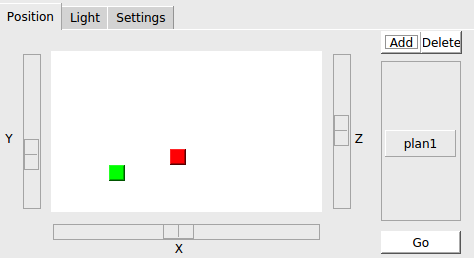
\includegraphics[width=0.9\linewidth]{0_Filer/Figuer/Position.png}
\caption{Position-tab}
\label{fig:GUI Position}
\end{figure}

\subsubsection{Light}
Light er den anden tab fra venstre mod højre, som kan ses i tab-widget menuen. Det er i denne tab, hvor interaktionen med lysstyring foretages. Selve vinduet er bygget op som en del af tab-widgetten i Displays's UI, men det er light.cpp, der står for behandlingen af interaktionerne, der sker i dette tab. 
Nedenfor ses et klassediagram for GUI'en, hvor klasserelationerne kan ses. Det fremgår af klasserelationerne, at Position som primære fil står for at hente data fra GUI'en og brugerens interaktionen med den, hvilket hovedsagligt foregår med signals \& slots. Signals \& slots er GUI'ens interne eventhandler. Når dette event sker, sendes dette signal til dette slot (funktion) som udfører det og det. QT er et eventbaseret system, så opbygningen af den er primært bestående af forståelsen for hvordan delelementer snakker sammen, eller snarer hvordan man får dem til at snakke sammen. Arv og pointerlogik spiller her en stor rolle.

\begin{figure}[H]
\centering
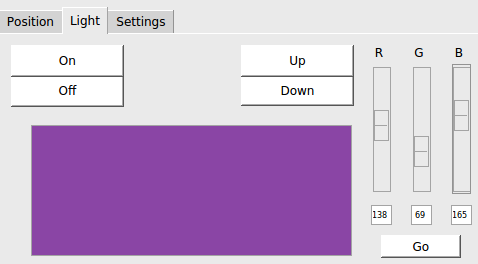
\includegraphics[width=0.9\linewidth]{0_Filer/Figuer/Light.png}
\caption{Light-tab}
\label{fig:GUI Light}
\end{figure}

\subsubsection{Settings}
Settings er den tredje tab fra venstre mod højre. Denne tab har til ansvar at sætte sensorindstillingerne. Disse sensorer indbefatter afstandssensor, bevælgelsessensor og lumensensor. Bevægelsessensoren og lumensensoren er helt simplistisk bestående af sliders som kan sættes til minumum, der beskriver tilstanden Off eller maksimum, der beskriver tilstande On. Når disse er On betyder det at sensorne er aktive og deres respons på virker udfaldsforløbet. Afstandssensoren er opbygget med af en spinbox, hvori man kan indstille hvilken afstand den skal registrere at et objekt er for tæt på. Dette er en heltalsværdi med minimum på 3 og maximum på 255 med enheden centimeter. Det er også i denne tab at kalibreringsknappen ”Calibrate” kan findes. Calibrate er noget brugeren kan benytte til at rette op på uoverensstemmelser i positionering hvis denne er skredet fra det forventet. Dette påbegynder en bevægelsesrutine og lagrer ved afslutning nogle calibreringsdata på de respektive slave PSoC'er, PSoC-XY og PSoC-Z.

\begin{figure}[H]
\centering
\includegraphics[width=0.9\linewidth]{0_Filer/Figuer/Settings.png}
\caption{Settings-tab}
\label{fig:GUI Position}
\end{figure}

\subsubsection{PlannerDialog og planner}
Plannerdialogboksen er den dialogboks der bringes frem, når man trykker på Add-knappen, hvis brugeren vælger at oprette en plan der skal gemmes. Dialogboksen indeholder et tekstfelt hvori navnet på planen indtastes. Der kan heri indtastes alle tegntyper begrænset til maksimalt 8-tegn. Dette antal er valgt for at de oprettede knapper har et navn det fylder maksimalt en linje med en skriftstørrelse, der vil være læsbar på et display af den størrelse der benyttes til dette produkt (480*272). Alt over 8-tegn ville kræve at skriftstørrelsen skulle være mindre eller der skulle laves linjeskift, hvilket ikke ville være hensigtsmæssigt. Indtastningen i indtastningsfeltet gøres vha. af det virtuelle keyboard, der befinder sig i den nederste halvdel af skærmen i dialogboksen. 

Keyboardet er ikke lavet af denne gruppe, men er blevet downloadet og implementeret fra "the Free Software Foundation". Keyboardet er dog blevet modificeret i størrelse og indtastningsvenlighed, og "Hide"-knappen der oprindeligt skulle benyttes til at skjule keyboardet er blevet gjort funktionsløst, da denne funktionalitet var unødvendig for dette produkt. For mere information om dette keyboard samt et downloadlink til det kan ses fra følgende reference\#. Under indtastningsfeltet kan findes en Ok- og Cancel-knap. Tryk på Ok-knappen opretter planen med det indtastede navn, hvorimod Cancel-knappen annulerer oprettelse af plan og returnere brugeren til den forhenværende brugerflade. For at undgå at navneløse planer bliver oprettet er Ok-knappen disablet indtil mindst et eller flere tegn indtastes i indtastningsfeltet. Der er en begrænsning på mængden af planer på 4, da dette var den maksimale mængde, der var plads til foruden knapstørrelsen skulle formindskes. Hvis en plan ønskes fjernet skal brugeren trykke på givne plan og trykke på Delete-knappen placeret ved siden af Add-knappen.

\begin{figure}[H]
\centering
\includegraphics[width=0.9\linewidth]{0_Filer/Figuer/plannerDialog.png}
\caption{Settings-tab}
\label{fig:GUI Dialog}
\end{figure}

% 6.1.2.4 Klassebeskrivelser Devkit8000
\subsection{Klassebeskrivelse Devkit8000}

MainDisplay er den første UI, som åbnes, når applikationen startes og det eneste, som forbliver åbent. Det er applikationens primære UI-fil, hvor den hovedsaglige interaktion foretages og fungerer som bindeled for GUI'ens klasser. Denne QWidget indeholder en stor række af GUI'ens funktionaliteter da GUI'en blev opbygget i tabs i stedet for i seperate QWidgets. MainDisplay's UI-fil indeholder den grundlæggende funktionalitet, som er nødvendig for at oprette vinduet.
\newline

Nedenfor ses et klassediagram for GUI’en, hvor det fremgår, at MainDisplay er den ledende klasse med det UI, som de andre klasser bruges i. Det fremgår af klasserelationen, at MainDisplay som Main Window anvender GUI’ens resterende klasser, hvilket hovedsagligt foregår med signals \& slots. Position, Planner og Light har ikke deres egne QWidget klasser da de alle er bygget på MainDisplay QWidgeten, hvilket har resulteret i en stor samling af klasse i en fil.

\begin{figure}[H] \centering
    \fbox{\includegraphics[width=0.95\textwidth]{0_Filer/Figuer/guiClassDia.png}}
    \caption{GUI klassediagram}
    \label{fig:GUI klassediagram}
\end{figure}

% 6.1.2.5 GUI repræsentationsbeskrivelse
\subsection{GUI repræsentationsbeskrivelse}

Klassen Position består af følgende filer:
\begin{itemize}
\item display.ui
\item position.cpp
\item maindisplay.h
\end{itemize}

display.ui er den UI-fil der indeholder de grafiske elementer der kodes for og denne UI-fil kræver sin tilhørende headerfil maindisplay.h. Source-filen position.cpp er der hvor al funktionalitet kodes.
\newline

GUI-filen repræsenterer et vindue bestående af følgende elementer:
\begin{itemize}

\item Tab Widget - Indeholder tre separate tabs: Position, Light og Settings.

\item Sliders (Position-tab) – Til indstilling af lampens position i X-, Y- og Z-aksen i trin mellem 0 og 255.

\item Go-knap (Position-tab) – Til at udsende sliderværdierne for X, Y og Z til bevægelse af lampe.

\item Add-knap (Position-tab) - Til åbne dialogboksen til oprettelse af en plan.

\item Sliders (Light-tab) - Til indstilling af farven der udsendes til lampen i trin mellem 0 og 255.

\item Trinbokse (Light-tab og Position-tab) - Til visning af sliders trinværdi.

\item Farvepalette (Light-tab) - Hvor indstillede farve vises, der forventes at blive vist på lysenhed.

\item On/Off-knapper (Light-tab) – On-knap til at sætte RGB-LED’erne på sidste lysindstilling forinden den blev slukket og Off-knap for at slukke lyset.

\item Up/Down-knapper (Light-tab) - Bruges til at flytte farvesliders enten op eller ned med 5 steps.

\item Labels – Position: X, Y og Z til identifikation af hvilken slider der kontrollerer hvilken akse. Light: R, G og B til identifikation af sliders for farverne rød, grøn og blå.

\item Plot – Et X-, Y-koordinatsystem til visualisering af lampens nuværende position (med grønt ikon) og dens kommende position (rødt ikon), hvis sliders er blevet flyttet.

\item Lumen slider (Settings-tab) - En slider til at sende en tænd- eller slukbesked til lyssensoren.

\item Movement slider (Setttings-tab) - En slider til at sende en tænd- eller slukbesked til bevægelsessensoren.

\item Distance spinbox (Settings-tab) - En spinbox der sætter den værdi hvorindenfor afstandssensoren sender en advarsel.

\end{itemize}

I constructoren til klassen MainDisplay sker opsætningen af GUI'en, når den startes. Her får vi komponenter fra UI'et til at kommunikere sammen med signals \& slots. Dette gøres vha. connect() metoder, så der kan emittes signaler, hvorefter de tilhørende slots kaldes. I dette specifikke kodeudsnit ses hvordan slidernes signaler er blevet sat op. Alle sliderne fra de tre tabs connectes samtidig. Position, Light og Settings er dermed klar til intern kommunikation forinden metoderne kaldes.

\begin{figure}[H]
\centering
\includegraphics[width=0.9\linewidth]{0_Filer/Figuer/signalSlot.png}
\caption{Kodeudsnit af Signals \& Slots i MainDisplay's constructor}
\label{fig:signalSlot}
\end{figure}

{\centering \textbf{spi-api} \par}

\begin{table}[H]
    \centering
    \begin{tabular}{|l|}
    \hline
    \multicolumn{1}{|c|}{<<boundary>>} \\
    \multicolumn{1}{|c|}{\textbf{spi-api}} \\
    \hline
    \\
    \hline
    + txPacket(unsigned char* const, unsigned char* const) : int \\
    + rxPacket(unsigned char* const, unsigned int*) : int \\
    \hline
    \end{tabular}
    \caption{Klasse spi-api}
    \label{tab:classSpiApi}
\end{table}

\begin{labeling}{Attributter:}
\item[Ansvar:] At være et lag imellem \textit{applications}-laget og \textit{device driver}-laget ifa. et \textit{kernemodul} på DevKit8000 som står for SPI kommunikationen.
\item[Attributter:] Ingen.
\end{labeling}

\begin{labeling}{Beskrivelse:}
\item[int txPacket(unsigned char* const, unsigned char* const)]
\item[Parametre:] Modtager to unsigned char pointere som peger på hhv. kommandoen og dataen der skal sendes via SPI-netværket til PSoC master fra DevKit8000.
\item [Returværdi:] Retunere en int med værdien 0 ved succes ellers en negativ værdi i overenstemmelse med fejl-listen.
\item [Beskrivelse:] Metoden skal sende en kommando og dertilhørende data væredi som en pakke via SPI-netværket fra DevKit8000 til PSoC Master med en kommando og data.
\end{labeling}

\begin{labeling}{Beskrivelse:}
\item[int rxPacket(unsigned char* const, unsigned int*)]
\item[Parametre:] Modtager en unsigned char pointer og en unsigned int pointer som peger på hhv. kommandoen der skal sendes til, og dataen hvor retur værdien skal lageres, som sendes via SPI-netværket til PSoC master fra DevKit8000.
\item [Returværdi:] Retunere en int med værdien 0 ved succes ellers en negativ værdi i overenstemmelse med fejl-listen.
\item [Beskrivelse:] Metoden skal sende en data pakke med kommandoen og derefter aflæse retur data fra PSoC Master som lagers på den dertil angivet unsigned int pointer, via SPI-netværket fra DevKit8000 til PSoC Master og retur.
\end{labeling}

{\centering \textbf{Position} \par}

\begin{labeling}{Attributter:}
\item[Ansvar:] Tage imod brugerens valg af lampeposition ud fra sliderenes position i taben ved navn Position.
\item[Attributter:] qunt8 x\_: En unsigned 8-bit integer som bestemmer lampens x-værdi (til koordinatstyring). \\
quint8 y\_: En unsigned 8-bit integer som bestemmer lampens y-værdi (til koordinatstyring). \\
quint8 z\_: En unsigned 8-bit integer som bestemmer lampens z-værdi (til koordinatstyring).
\end{labeling}

\begin{labeling}{Beskrivelse:}
\item[struct setXYZ(quint8, quint8, quint8)]
\item [Parametre:] Unsigned int med x-værdi. \\
Unsigned int med y-værdi. \\
Unsigned int med z-værdi.
\item [Returværdi:] x, y og z’s sliderværdier til positionering.
\item [Beskrivelse:] En struct med ansvar for at sætte x-, y- og z-værdierne som skal sendes videre så motorerne kan styres i tre dimensioner.
\end{labeling}

\begin{labeling}{Beskrivelse:}
\item[void on\_PosChanged()]
\item[Parametre:] Ingen.
\item [Returværdi:] Ingen.
\item [Beskrivelse:] Metoden er et slot til sliderReleased() signaler og kaldes ved sliderReleaseEvent
(når en slider slippes efter brug). Den sætter koordinatværdier ud fra sliderpositioner i trin mellem 0 og 255. Disse sendes videre til lampepositionering.
\end{labeling}

\begin{labeling}{Beskrivelse:}
\item[void on\_calButton\_clicked()]
\item[Parametre:] Ingen.
\item [Returværdi:] Ingen.
\item [Beskrivelse:] Kalibrerer system ved først at set X, Y og Z til den maksimale værdi muligt og returnerer til positionen før kalibrering når opgaven er tilendebragt.
\end{labeling}

\begin{labeling}{Beskrivelse:}
\item[Display::\char`\~Display()]
\item[Parametre:] Ingen
\item [Returværdi:] Ingen
\item [Beskrivelse:] Destructor til nedlæggelse af det grafiske interface, når den kaldes
\end{labeling}

\begin{labeling}{Beskrivelse:}
\item[bool getCalStatus()]
\item[Parametre:] Ingen
\item [Returværdi:] En true eller false der beskriver om kalibrering forløber korrekt.
\item [Beskrivelse:] Hvis kalibrering forløber fejlfrit vil true blive returneret og ellers returneres false. En information, der kan bruges til fejlhåndtering.
\end{labeling}

\begin{labeling}{Beskrivelse:}
\item[void setStatusLine(const QString)]
\item[Parametre:] Et tekststykke der beskriver sidste handling udført.
\item [Returværdi:] Ingen.
\item [Beskrivelse:] En statuslinje der udskriver hvad status for systemet er lige nu.
\end{labeling}

{\centering \textbf{Light} \par}

\begin{labeling}{Attributter:}
\item[Ansvar:] Indstille lysets farve og intensitet for lampen.
\item[Attributter:] quint8 red\_: En unsigned 8-bit integer som bestemmer lampens røde farveintensitet.\\
quint8 green\_: En unsigned 8-bit integer som bestemmer lampens grønne farveintensitet. \\
quint8 blue\_: En unsigned 8-bit integer som bestemmer lampens blå farveintensitet.
\end{labeling}

\begin{labeling}{Beskrivelse:}
\item[struct setSliders(quint8, quint8, quint8)]
\item[Parametre:] Unsigned 8-bit integer med red\_. Unsigned 8-bit integer med green\_. Unsigned 8-bit integer med blue\_.
\item [Returværdi:] En struct med ansvar for at sætte R-, G- og B-værdierne, som skal sendes videre så RGB’ernes farveniveauer kan styres.
\item [Beskrivelse:] En struct med ansvar for at sætte red-, green- og blue-værdierne, som skal sendes videre til lampens RGB-LED’ers farve og lysintensitet. Alle farverne bestemmes med en trinværdi mellem 0 og 255.
\end{labeling}

\begin{labeling}{Beskrivelse:}
\item[void on\_upButton\_clicked()]
\item[Parametre:] Ingen.
\item [Returværdi:] Ingen.
\item [Beskrivelse:] Øger lampens lysintensitet ved at lægge en til alle farver (rød, grøn og blå), ved klik på Up-knappen i GUI’ens Light-tab.
\end{labeling}

\begin{labeling}{Beskrivelse:}
\item[void on\_downButton\_clicked()]
\item[Parametre:] Ingen.
\item [Returværdi:] Ingen.
\item [Beskrivelse:] Sænker lampens lysintensitet ved trække en fra alle farver (rød, grøn og blå), ved klik på Down-knappen i GUI’ens Light-tab.
\end{labeling}

\begin{labeling}{Beskrivelse:}
\item[void on\_onButton\_clicked()]
\item[Parametre:] Ingen.
\item [Returværdi:] Ingen.
\item [Beskrivelse:] Tænder lampens lys med sidst benyttede intensitet, ved klik på On-knappen i GUI’ens Light-tab.
\end{labeling}

\begin{labeling}{Beskrivelse:}
\item[void on\_offButton\_clicked()]
\item[Parametre:] Ingen.
\item [Returværdi:] Ingen.
\item [Beskrivelse:] Slukker lampens lys ved klik på Off-knappen i GUI’ens Light-tab.
\end{labeling}

\begin{labeling}{Beskrivelse:}
\item[void updatePalette(QColor\&)]
\item[Parametre:] Reference til farve som Color Preview sættes med.
\item [Returværdi:] En struct med ansvar for at sætte R-, G- og B-værdierne som skal sendes videre så RGB’ernes farveniveauer kan styres.
\item [Beskrivelse:] En struct med ansvar for at sætte red-, green- og blue-værdierne, som skal sendes videre til lampens RGB-LED’ers farve og lysintensitet. Alle farverne bestemmes med en trinværdi mellem 0 og 255.
\end{labeling}

\begin{labeling}{Beskrivelse:}
\item[bool lightSens()]
\item[Parametre:] Ingen.
\item [Returværdi:] True hvis lyssensorens input skal behandles eller false hvis kommunikation med lyssensor er deaktiveret.
\item [Beskrivelse:] Der vil her blive angivet og hvor vidt kommunikation med lyssensoren vil blive behandlet.
\end{labeling}

\subsection{GUI modultest}
Der er blevet lavet en række forskellige test på GUI'en for at sikre at alle funktionerne har de korrekte funktionaliteter. Koden indeholder mange metoder og interne signaler der skal sendes rigtigt hele vejen igennem systemet for at sikre at resten af systemet vil kunne bruge de udsendte data. GUI test er primært blevet fortaget med QDebugger som bliver brugt til at udskrive data og tekststrenge for at de kunne følge kodens forløb. \newline

\begin{table}[H]
\begin{tabular}{|l|l|}\hline
\textbf{Test} & Positionsindstilling ved sliderændringer \\\hline

\textbf{Testbeskrivelse} & \multicolumn{1}{|m{11.5cm}|}{Det testes, om ændring af X-, Y- og Z-sliders positioner sætter nogle værdier og om de bliver sendt korrekt ved tryk på Go-knap.  QDebug() bruges til at udskrive positionsværdierne i metoden on\_PosChanged(), der kaldes ved valueChanged(int).} \\\hline


\textbf{Input} & \multicolumn{1}{|m{11.5cm}|}{Sliders positioner ændres til hhv. 255, 255, 255. Derefter trykkes Go-knappen ned og slippes igen.} \\\hline

\textbf{Output} & \multicolumn{1}{|m{11.5cm}|}{ Sliderpositionen og nuværende position vil ændre sig til "255, 255, 255", blive udskrevet og de negative kommandokoder vil blive returneret som fejlkoder (X=16, Y=17, Z=32).} \\\hline

\textbf{Resultat} & \multicolumn{1}{|m{11.5cm}|}{ OK} \\\hline

\end{tabular}
\end{table}

\begin{figure}[H]
\centering
\includegraphics[width=0.9\linewidth]{0_Filer/Figuer/testPosition.png}
\caption{Debug output ved sliderværdierne (X, Y, Z): 255, 255, 255, den sendte værdi currentpos: 255, 255, 255 og negative sendte kommandoer.}
\label{fig:testPosition}
\end{figure}


\begin{table}[H]
\begin{tabular}{|l|l|}\hline
\textbf{Test} & Lysindstilling ved sliderændringer \\\hline

\textbf{Testbeskrivelse} & \multicolumn{1}{|m{11.5cm}|}{Det testes, om ændring af R-, G- og B-sliders positioner sætter nogle værdier og om de bliver sendt korrekt ved tryk på Go-knap.  QDebug() bruges til at udskrive positionsværdierne i metoden on\_ColorChanged(), der kaldes ved valueChanged(int).} \\\hline

\textbf{Input} & \multicolumn{1}{|m{11.5cm}|}{Sliders positioner ændres til hhv. 255, 255, 255. Derefter trykkes Go-knappen ned og slippes igen.} \\\hline

\textbf{Output} & \multicolumn{1}{|m{11.5cm}|}{ Sliderpositionen og sendte lysværdi vil ændre sig til "255, 255, 255", blive udskrevet og de negative kommandokoder vil blive returneret som fejlkoder (R=48, G=49, B=50).} \\\hline

\textbf{Resultat} & \multicolumn{1}{|m{11.5cm}|}{ OK} \\\hline

\end{tabular}
\end{table}

\begin{figure}[H]
\centering
\includegraphics[width=0.9\linewidth]{0_Filer/Figuer/testLight.png}
\caption{Debug output ved sliderværdierne Color values (R, G, B): 255, 255, 255, den sendte værdi Sending color: 255, 255, 255 og negative sendte kommandoer.}
\label{fig:testLight}
\end{figure}



\begin{table}[H]
\begin{tabular}{|l|l|}\hline
\textbf{Test} & Sensorindstilling ved slider og spinboxændringer \\\hline

\textbf{Testbeskrivelse} & \multicolumn{1}{|m{11.5cm}|}{Det testes, om ændring af Movementslider og Lumensensor samt Distancespinbox bliver sendt videre med spi kommandoer.} \\\hline

\textbf{Input} & \multicolumn{1}{|m{11.5cm}|}{Sliders position for Movement og Lumen ændres fra Off til On. Derefter ændres Distancespinboxværdien til 4.} \\\hline

\textbf{Output} & \multicolumn{1}{|m{11.5cm}|}{ Sliderpositioner for Lumen og Movement ændres til On, status bliver udskrevet og de negative kommandokoder vil blive returneret som fejlkoder (R=48, G=49, B=50).} \\\hline

\textbf{Resultat} & \multicolumn{1}{|m{11.5cm}|}{ OK} \\\hline

\end{tabular}
\end{table}

\begin{figure}[H]
\centering
\includegraphics[width=0.9\linewidth]{0_Filer/Figuer/testSettings.png}
\caption{Debug output ved sliderværdierne Lumen value: 1, Movement value: 1, spinboxværdien Distance value: 4 og negative sendte kommandoer.}
\label{fig:testSettings}
\end{figure}



\begin{table}[H]
\begin{tabular}{|l|l|}\hline
\textbf{Test} & Oprettelse af plan \\\hline

\textbf{Testbeskrivelse} & \multicolumn{1}{|m{11.5cm}|}{Det testes, om der kan oprettes en plan og de korrekte værdier gemmes.} \\\hline

\textbf{Input} & \multicolumn{1}{|m{11.5cm}|}{Sliderposition for X, Y og Z ændres til "255, 255, 255" og R, G, og B ændres til "255, 0, 0". Der trykkes dernæst op Add-knappen, et navn indtastes i dialogboksen der fremvises på skærmen og Ok-knappen trykkes.} \\\hline

\textbf{Output} & \multicolumn{1}{|m{11.5cm}|}{Plannens positionsvædier sættes til "255, 255, 255" og lysværdierne sættes til "255, 0, 0". Disse værdier udskrives i debuggeren.} \\\hline

\textbf{Resultat} & \multicolumn{1}{|m{11.5cm}|}{ OK} \\\hline

\end{tabular}
\end{table}

\begin{figure}[H]
\centering
\includegraphics[width=0.9\linewidth]{0_Filer/Figuer/testMakePlan.png}
\caption{Debug output ved satte plan X, Y og Z Setting plan position: (255, 255, 255), lyset R, G, B Setting plan Light (255, 0, 0) og Setting according to plan}
\label{fig:testmakePlan}
\end{figure}

\clearpage
\clearpage

% 7. Accepttest
% 7. Accepttest
\chapter{Accepttest}

\begin{table}[!htbp] \centering
\begin{tabular}{|p{2cm}|p{8cm}|}
	\hline
		\multicolumn{2}{|l|}{Versionshistorik} \\\hline
		\textbf{v1.0} &15-03-2016 Pre-review\\\hline
	\end{tabular}
\end{table}

Punkterne i Accepttestspecifikationen, er skrevet ud fra punkterne i hovedforløbet, for de enkelte usecases.

\section{Testopstilling}

\begin{figure}[H]
\centering
\includegraphics[width=1.0\linewidth]{0_Filer/Figuer/testopstilling.png}
\caption{Testopstillingsbillede}
\label{fig:testopstilling}
\end{figure}

En tændt computer med Teraterm åbent tilsluttes med USB til PSoC Master for at kontrollere at kommunikationen igennem hele systemet forløber korrekt. Et Devkit8000 med GUI’en aktivt kørende tilsluttes med de korrekte ledningsforbindelser til PSoC Master. Devkit8000 tilkobles en PC koblet på Devkittet til aflæsning af qDebug returværdier. På PSoC Masteren tilsluttes et Nokia 5150 display til udskrivning af modtaget beskeder til postkontoret. Til PSoC Masteren tilkobles de tre PSoC slaver: PSoC Z, PSoC XY og PSoC Sensor i nævnte rækkefølge fra venstre mod højre og alle tre monteret Unified Board som anvist på testopstillingsbilledet. Ledningsforbindelserne fra Unified Board tilsluttes til resten af systemet med ledninger og fladkabel.

% Accepttest Use Case 1
\section{ATUC1: Kalibrér system}

\begin{center} \centering
    \begin{longtable}{|p{0,5cm}|p{3,7cm}|p{3,7cm}|p{2,3cm}|p{2,3cm}|}
    \hline
        \multicolumn{5}{|l|}{\textbf{ATUC1: Kalibrer system}} \\ \hline
        \multicolumn{1}{|c|}{} &
        \textbf{Test} &
        \textbf{Forventet \newline Resultat} &
        \textbf{Resultat} &
        \textbf{Godkendt\slash \newline Kommentar} \\ \hline 
        \endfirsthead

        \multicolumn{5}{l}{...fortsat fra forrige side} \\ \hline 
        \multicolumn{5}{|l|}{\textbf{ATUC1: Kalibrer system}} \\ \hline
        \multicolumn{1}{|c|}{} &
        \textbf{Test} &
        \textbf{Forventet \newline Resultat} &
        \textbf{Resultat} &
        \textbf{Godkendt\slash \newline Kommentar} \\ \hline 
        \endhead
        
        \multicolumn{5}{r}{fortsættes på næste side...} \\
        \endfoot
        \endlastfoot

        \textbf{1} 
            & Brugeren trykker ”Calibrate”-knap på touchskærmen under Settings-tabben.
            & Lampen trækkes helt op og bliver så kørt helt frem og tilbage i først X-dimensionen og dernæst Y-dimensionen. Disse kalibreringsværdier forventes returneret og gemt til de pågældende PSoC'er.
            & Kalibreringsrutinen blev tilendebragt i alle tre akser fejlfrit og kalibreringsdata blev gemt.	
            & Godkendt. 
        \\ \hline
	\end{longtable}
	\label{ATUC1} 
\end{center}

% Accepttest Use Case 2
\section{ATUC2: Tænd/sluk lys}

\begin{center} \centering
    \begin{longtable}{|p{0,5cm}|p{3,7cm}|p{3,7cm}|p{2,3cm}|p{2,3cm}|}
    \hline
        \multicolumn{5}{|l|}{\textbf{ATUC2: Tænd/sluk lys}} \\ \hline
        \multicolumn{1}{|c|}{} &
        \textbf{Test} &
        \textbf{Forventet \newline Resultat} &
        \textbf{Resultat} &
        \textbf{Godkendt\slash \newline Kommentar} \\ \hline 
        \endfirsthead

        \multicolumn{5}{l}{...fortsat fra forrige side} \\ \hline 
        \multicolumn{5}{|l|}{\textbf{ATUC2: Tænd/sluk lys}} \\ \hline
        \multicolumn{1}{|c|}{} &
        \textbf{Test} &
        \textbf{Forventet \newline Resultat} &
        \textbf{Resultat} &
        \textbf{Godkendt\slash \newline Kommentar} \\ \hline 
        \endhead

        \multicolumn{5}{r}{fortsættes på næste side...} \\
        \endfoot
        \endlastfoot
        
        \textbf{1} 
            & Brugeren indstiller en tilfældig farve med R-, G- og B-sliderne i Light-tabben.
            & Lyspaletten på touchskærmen opdateres til en farve i overensstemmelse med de indstillede sliderværdier.
            & Lyspaletten blev opdateret til valgte værdig
            &  Godkendt.
        \\ \hline
        \textbf{2} 
            & Brugeren trykker på Go-knappen placeret under R-, G- og B-sliderne.
            & Lampens lys bliver sat til den samme farve som den fremviste på touchskærmen.
            & Lampens lys stemte overens med farvepaletten.
            & Godkendt.
        \\ \hline
        \textbf{3} 
            & Brugeren trykker på ”On/Off”-knap på touchskærmen under Light-tabben på touchskærmen.
            & Lyset skifter tilstand, fra tændt til slukket, eller fra slukket til tændt med valgte sliderfarve.
            & Lyset slukkede ved tryk på Off-knappen og tændte igen ved tryk på On-knappen.
            & Godkendt.
        \\ \hline
	\end{longtable}
	\label{ATUC2}
\end{center}

% Accepttest Use Case 3
\section{ATUC3: Registrér bevægelse}

\begin{center} \centering
    \begin{longtable}{|p{0,5cm}|p{3,7cm}|p{3,7cm}|p{2,3cm}|p{2,3cm}|}
    \hline
        \multicolumn{5}{|l|}{\textbf{ATUC3: Registrér bevægelse}} \\ \hline
        \multicolumn{1}{|c|}{} &
        \textbf{Test} &
        \textbf{Forventet \newline Resultat} &
        \textbf{Resultat} &
        \textbf{Godkendt\slash \newline Kommentar} \\ \hline 
        \endfirsthead

        \multicolumn{5}{l}{...fortsat fra forrige side} \\ \hline 
        \multicolumn{5}{|l|}{\textbf{ATUC3: Registrér bevægelse}} \\ \hline
        \multicolumn{1}{|c|}{} &
        \textbf{Test} &
        \textbf{Forventet \newline Resultat} &
        \textbf{Resultat} &
        \textbf{Godkendt\slash \newline Kommentar} \\ \hline 
        \endhead

        \multicolumn{5}{r}{fortsættes på næste side...} \\
        \endfoot
        \endlastfoot
        
        \textbf{1} 
            & Bruger sætter Movement detection slideren til On på touchdisplayet under Sensor-tabben.
            & Slideren skifter position til On-positionen og bliver grøn.
            & Slideren skiftede til korrekt position og farve.	
            & Godkendt.
        \\ \hline
        \textbf{2} 
            & Bruger fører en arm forbi bevægelsessensoren på en afstand mindre end den fastsatte værdi under "Distance limit" spinboxen på touch displayet's Sensor-tab.
            & Lyset tændes med samme farve som angivet på Light-tabbens farvepalette på touchskærmen.
            & Lyset blev tændt med den samme værdi som den valgte Light-tabben.	
            & Godkendt. 
        \\ \hline
	\end{longtable}
	\label{ATUC3}
\end{center}

% Accepttest Use Case 4
\section{ATUC4: Justér lysets farve }

\begin{center} \centering
    \begin{longtable}{|p{0,5cm}|p{3,7cm}|p{3,7cm}|p{2,3cm}|p{2,3cm}|}
    \hline
        \multicolumn{5}{|l|}{\textbf{ATUC4: Justér lysets farve }} \\ \hline
        \multicolumn{1}{|c|}{} &
        \textbf{Test} &
        \textbf{Forventet \newline Resultat} &
        \textbf{Resultat} &
        \textbf{Godkendt\slash \newline Kommentar} \\ \hline 
        \endfirsthead

        \multicolumn{5}{l}{...fortsat fra forrige side} \\ \hline 
        \multicolumn{5}{|l|}{\textbf{ATUC4: Justér lysets farve }} \\ \hline
        \multicolumn{1}{|c|}{} &
        \textbf{Test} &
        \textbf{Forventet \newline Resultat} &
        \textbf{Resultat} &
        \textbf{Godkendt\slash \newline Kommentar} \\ \hline 
        \endhead

        \multicolumn{5}{r}{fortsættes på næste side...} \\
        \endfoot
        \endlastfoot
        
        \textbf{1} 
            & Brugeren sætter fingeren på rød farve-slideren "R"  på touchskærmen.
            & Slideren følger fingeren op og ned.
            & Slideren følger fingeren op og ned på "R"slideren.	
            &  Godkendt.
        \\ \hline
        \textbf{2} 
            & Brugeren trækker slideren helt til minimum (0) og trykker dernæst på Go-knappen under farvesliderne.
            & Den korresponderende farve i lampens diode slukkes helt.
            & Farven i lampens diode dæmpes for rød. 	
            & Godkendt.
        \\ \hline
        \textbf{3} 
            & Brugeren trækker slideren helt til maximum (255) og trykker dernæst på Go-knappen under farvesliderne.
            & Den korresponderende farve i lampens diode forstærkes til maksimal lysstyrke.
            & Farven i lampens diode forstærkes for rød.	
            & Godkendt.
        \\ \hline
        \textbf{4} 
            & Brugeren gentager trin 1 til 3 med grøn farve-slideren "G" og blå farve-slideren "B".
            & Samme resultater forventes for alle farver.
            & Samme resultat ses for alle tre farver.	
            & Godkendt.
        \\ \hline
	\end{longtable}
	\label{ATUC4}
\end{center}

% Accepttest Use Case 5
\section{ATUC5: Indstil placering af lampen}

\begin{center} \centering
    \begin{longtable}{|p{0,5cm}|p{3,7cm}|p{3,7cm}|p{2,3cm}|p{2,3cm}|}
    \hline
        \multicolumn{5}{|l|}{\textbf{ATUC5: Indstil placering i loft}} \\ \hline
        \multicolumn{1}{|c|}{} &
        \textbf{Test} &
        \textbf{Forventet \newline Resultat} &
        \textbf{Resultat} &
        \textbf{Godkendt\slash \newline Kommentar} \\ \hline 
        \endfirsthead

        \multicolumn{5}{l}{...fortsat fra forrige side} \\ \hline 
        \multicolumn{5}{|l|}{\textbf{ATUC5: Indstil placering af lampen}} \\ \hline
        \multicolumn{1}{|c|}{} &
        \textbf{Test} &
        \textbf{Forventet \newline Resultat} &
        \textbf{Resultat} &
        \textbf{Godkendt\slash \newline Kommentar} \\ \hline 
        \endhead

        \multicolumn{5}{r}{fortsættes på næste side...} \\
        \endfoot
        \endlastfoot
        
        \textbf{1} 
            & Brugeren trækker i Y-slideren i opadgående retning på touchskærmens Position-fane.
            & Det røde ikon på touchskærmens Position-fane bevæger sig i opadgående retning og Y-sliderens tilhørende talværdi opdateres til en højere talværdi en den forhenværende.
            & Det røde ikon bevægede sig opad i takt med at Y-slideren bevægede sig opad. Talværdien blev opdateret til en forøget værdi.
            & Godkendt.
        \\ \hline
        \textbf{2} 
            & Brugeren trækker i Y-slideren i nedadgående retning på touchskærmens Position-fane.
            & Det røde ikon på touchskærmens Position-fane bevæger sig i opadgående retning og Y-sliderens tilhørende talværdi opdateres til en lavere talværdi en den forhenværende.
            & Det røde ikon bevægede sig nedad i takt med at Y-slideren bevægede sig opad. Talværdien blev opdateret til en formindsket værdi.
            & Godkendt.
        \\ \hline
        \textbf{3} 
            & Brugeren trækker i X-slideren i retningen mod højre på touchskærmens Position-fane.
            & Det røde ikon på touchskærmens Position-fane bevæger sig i retningen mod højre og X-sliderens tilhørende talværdi opdateres til en højere talværdi en den forhenværende.
            & Det røde ikon bevægede sig mod højre i takt med at X-slideren bevægede sig mod højre. Talværdien blev opdateret til en forøget værdi.
            & Godkendt
        \\ \hline
        \textbf{4} 
            & Brugeren trækker i X-slideren i retningen mod venstre på touchskærmens Position-fane.
            & Det røde ikon på touchskærmens Position-fane bevæger sig i retningen mod venstre og X-sliderens tilhørende talværdi opdateres til en lavere talværdi en den forhenværende.
            & Det røde ikon bevægede sig mod højre i takt med at X-slideren bevægede sig mod højre. Talværdien blev opdateret til en formindsket værdi.	
            & Godkendt 
        \\ \hline
        \textbf{5} 
            & Brugeren trækker i Z-slideren i opadgående retning på touchskærmens Position-fane.
            & Z-sliderens tilhørende talværdi opdateres til en højere talværdi en den forhenværende.
            & Talværdien blev opdateret til en forøget værdi.	
            & Godkendt. 
        \\ \hline
        \textbf{6} 
            & Brugeren trækker i Z-slideren i nedadgående retning på touchskærmens Position-fane.
            & Z-sliderens tilhørende talværdi opdateres til en lavere talværdi en den forhenværende.
            & Talværdien blev opdateret til en formindsket værdi.
            & Godkendt. 
        \\ \hline
        \textbf{7} 
            & Brugeren trykker på Go-knappen på touchskærmens Position-fane.
            & Et grønt ikon dækker det røde ikon og lampen bevæger sig nu afhængigt af de nu valgte sliderpositioner for X, Y og Z.
            & Et grønt ikon dækkede det røde ikon og lampen bevægede sig afhængigt af de valgte X-, Y- og Z-værdier.	
            & Godkendt. 
        \\ \hline
	\end{longtable}
	\label{ATUC5}
\end{center}

% Accepttest Use Case 6
\input{7_Accepttest/atuc6}

% Accepttest Use Case 7
\input{7_Accepttest/atuc7}

% Accepttest Use Case 8
%\section{ATUC8: Tilføj plan}

\begin{center} \centering
    \begin{longtable}{|p{0,5cm}|p{3,7cm}|p{3,7cm}|p{2,3cm}|p{2,3cm}|}
    \hline
        \multicolumn{5}{|l|}{\textbf{ATUC8: Tilføj plan}} \\ \hline
        \multicolumn{1}{|c|}{} &
        \textbf{Test} &
        \textbf{Forventet \newline Resultat} &
        \textbf{Resultat} &
        \textbf{Godkendt\slash \newline Kommentar} \\ \hline 
        \endfirsthead

        \multicolumn{5}{l}{...fortsat fra forrige side} \\ \hline
        \multicolumn{5}{|l|}{\textbf{ATUC8: Tilføj plan}} \\ \hline
        \multicolumn{1}{|c|}{} &
        \textbf{Test} &
        \textbf{Forventet \newline Resultat} &
        \textbf{Resultat} &
        \textbf{Godkendt\slash \newline Kommentar} \\ \hline 
        \endhead

        \multicolumn{5}{r}{fortsættes på næste side...} \\
        \endfoot
        \endlastfoot
        
        \textbf{1} 
            & Brugeren klikker ”Planner” fanen på Devkit8000-touchskærmen.
            & ”Planner” fanen vises på Devkit8000-touchskærmen. 
            & 	
            &  
        \\ \hline
        \textbf{2} 
            & Brugeren klikker på ”Save location”-knappen på Devkit8000-touchskærmen.
            & Devkit8000-touchskærmen beder brugeren om at indtaste et navn.
            & 	
            &  
        \\ \hline
        \textbf{3} 
            & Brugeren indtaster et navn på 10 tegn og trykker på ”Save” knappen
            & Systemet giver besked om at positionen er gemt i systemet. 
            & 	
            &  
        \\ \hline
	\end{longtable}
	\label{ATUC8}
\end{center}

% Accepttest Use Case 9
%\section{ATUC9: Vælg plan}

\begin{center} \centering
    \begin{longtable}{|p{0,5cm}|p{3,7cm}|p{3,7cm}|p{2,3cm}|p{2,3cm}|}
    \hline
        \multicolumn{5}{|l|}{\textbf{ATUC9: Vælg plan}} \\ \hline
        \multicolumn{1}{|c|}{} &
        \textbf{Test} &
        \textbf{Forventet \newline Resultat} &
        \textbf{Resultat} &
        \textbf{Godkendt\slash \newline Kommentar} \\ \hline 
        \endfirsthead

        \multicolumn{5}{l}{...fortsat fra forrige side} \\ \hline 
        \multicolumn{5}{|l|}{\textbf{ATUC9: Vælg plan}} \\ \hline
        \multicolumn{1}{|c|}{} &
        \textbf{Test} &
        \textbf{Forventet \newline Resultat} &
        \textbf{Resultat} &
        \textbf{Godkendt\slash \newline Kommentar} \\ \hline 
        \endhead

        \multicolumn{5}{r}{fortsættes på næste side...} \\
        \endfoot
        \endlastfoot
        
        \textbf{1} 
            & Brugeren klikker på ”Planner” fanen på Devkit8000-touchskærmen.
            & ”Planner” fanen vises på Devkit8000-touchskærmen.
            & 	
            &  
        \\ \hline
        \textbf{2} 
            & Brugeren klikker på en gemt plan på Devkit8000-touchskærmen.
            & En meddelelse om at en plan er valgt vises på Devkit8000-touchskærmen.
            & 	
            &  
        \\ \hline
	\end{longtable}
	\label{ATUC9}
\end{center}

% Referencelist
\clearpage
\printbibliography[heading=bibintoc,title={Referenceliste}]

\end{document}